%search for nnnote for things to resolve later.

\RequirePackage[l2tabu, orthodox]{nag}

\documentclass[letterpaper, 10 pt]{report}

%\usepackage[sc]{mathpazo}
%\linespread{1.05}

\usepackage{garamondx}
\usepackage[garamondx,cmbraces]{newtxmath}

\usepackage[T2A, T1]{fontenc}
\usepackage[utf8]{inputenc}
\usepackage{CJKutf8}
\usepackage{amsfonts}
\usepackage{amsmath}
\usepackage{amssymb}
\usepackage{braket}
\usepackage{ellipsis}
\usepackage{microtype}
\usepackage{graphicx}
\usepackage{caption}
\usepackage{subcaption}
\usepackage[usenames,dvipsnames]{xcolor}
\usepackage{setspace}
\usepackage[sc]{titlesec}
\usepackage[doi = false, url = false, isbn = false,
            maxbibnames = 99, sorting = none, backend = bibtex,
            giveninits = true, style = numeric-comp]{biblatex}
\usepackage[colorlinks, breaklinks=true]{hyperref}
\usepackage[toc,page]{appendix}

\usepackage{showlabels}

%\titleformat{\chapter}{\normalfont\huge}{\thechapter.}{20pt}{\huge}

%change link colours:
\hypersetup{ linktocpage, colorlinks=true, linkcolor=blue,
             citecolor=blue, filecolor=blue, urlcolor=blue }

%Bibliography stuff:
\addbibresource{diss.bib}

%Make titles a link:
\newbibmacro{string+doiurlisbn}[1]{%
   \iffieldundef{doi}{%
      \iffieldundef{url}{%
         \iffieldundef{isbn}{%
            \iffieldundef{issn}{%
               #1%
            }{%
               \href{http://books.google.com/books?vid=ISSN\thefield{issn}}{#1}%
            }%
         }{%
            \href{http://books.google.com/books?vid=ISBN\thefield{isbn}}{#1}%
         }%
      }{%
         \href{\thefield{url}}{#1}%
      }%
   }{%
      \href{http://dx.doi.org/\thefield{doi}}{#1}%
   }%
}

\DeclareFieldFormat{title}{\usebibmacro{string+doiurlisbn}{\mkbibemph{#1}}}
\DeclareFieldFormat[article,incollection]{title}%
   {\usebibmacro{string+doiurlisbn}{\mkbibquote{#1}}}


\title{Dissertation: early version}
\author{Matthew Baxter}
\date{\today}

\begin{document}

\pagenumbering{alph}

\begin{titlepage} %nnnote: fix this later.

   \centering
   
   {\Large Title\dots}
   
   \vspace{2 cm}
   
   \textsc{matthew baxter}
   
   \vspace{2 cm}
   
   \textsc{a thesis submitted to the faculty of graduate studies in partial fulfillment of the
           requirements for the degree of master of science}
   
   \vspace{2 cm}
   
   \textsc{graduate programme in the department of physics and astronomy}
   
   \textsc{york university}
   
   \textsc{toronto ontario}
   
   Month Year
   
   \vspace{3.5 cm}
   
   \copyright Matthew Baxter, 2012.   

   \thispagestyle{empty}

\end{titlepage}

\cleardoublepage
\phantomsection
\addcontentsline{toc}{chapter}{Abstract}

\begin{abstract}
   
   \thispagestyle{plain}
   \pagenumbering{roman}
   \setcounter{page}{2}

\end{abstract}

\setcounter{page}{3}

\cleardoublepage
\phantomsection
\addcontentsline{toc}{chapter}{Contents}
\tableofcontents

\cleardoublepage
\phantomsection
\addcontentsline{toc}{chapter}{List of Tables}
\listoftables

\cleardoublepage
\phantomsection
\addcontentsline{toc}{chapter}{List of Figures}
\listoffigures

\newpage

\pagenumbering{arabic}

\onehalfspacing  %spacing here

\begin{chapter}{Introduction \label{chap:intro}}

\end{chapter}

\begin{chapter}{Density Functional Theory \label{chap:dft}}

   This chapter concerns itself with a brief introduction to the world of density-functional theory,
   both ground-state~\cite{dft-engel} (\textsc{dft}) and time-dependent~\cite{tddft, marques-1}
   (\textsc{tddft}). This discussion begins with a discussion of various existence theorems central to
   density functional theory (Sec.~\ref{sec:dft}). Next the Kohn-Sham equations are introduced in
   Sec.~\ref{sec:ks}. More practical matters are considered when the two main problems of density
   functional theory, the observable problem (Sec.~\ref{sec:obs}) and the determination of the
   exchange-correlation potential (Sec.~\ref{sec:xcpot}) are introduced. The discussion of the
   xc-potential is focused on the optimized potential method (Sec.~\ref{sec:opm}) and the
   Krieger-Li-Iafrate approximation (Sec.~\ref{sec:kli}).

   \begin{section}{\textsc{dft} and \textsc{tddft} Existence Theorems \label{sec:dft}}

      In the standard treatment of many-body quantum mechanics a system is described by a wavefunction
      $\Psi$ which, depending upon the situation, is determined by either the time-dependent
      Schr\"{o}dinger equation (\textsc{tdse})
      %
      \begin{equation} \label{eq:tdse}
         \hat{H}(t) \Psi(t) = i \frac{\mathrm{d} \Psi(t)}{\mathrm{d} t},
      \end{equation}
      %
      or the stationary Schr\"{o}dinger equation (\textsc{sse})
      %
      \begin{equation} \label{eq:sse}
         \hat{H} \Psi = E \Psi.
      \end{equation}
      %
      If the system in question consists of $N$ non-relativistic electrons then $\Psi$ becomes a
      function of $N$ position variables $\mathbf{r}_i$ and spin variables $\sigma_i$. The Hamiltonian,
      $\hat{H}$, may be decomposed into a kinetic energy term
      %
      \begin{equation} \label{eq:Top} %nnnote: tfrac or normal frac?
         \hat{T} = -\frac{1}{2} \sum\limits^{N}_{i=1} \Delta_i,
      \end{equation}
      %
      an electron-electron term
      %
      \begin{equation} \label{eq:Vee} %nnnote: tfrac or normal frac?
         \hat{V}_{ee} = \frac{1}{2} \sum\limits^{N}_{i \neq j}
                        \frac{1}{\left| \mathbf{r}_i - \mathbf{r}_j \right|},
      \end{equation}
      %
      and a, possibly, time-dependent external potential
      %
      \begin{equation} \label{eq:Vext}
         \hat{V}_\mathrm{ext} = \sum\limits^{n}_{i = 1} v_\mathrm{ext} (\mathbf{r}_i, \sigma_i, t).
      \end{equation}
      %
      The function $\hat{V}_\mathrm{ext}$ contains all of the one-body interactions, including the
      nuclear and any external potentials.

      Given the one-particle electronic density
      %
      \begin{equation} \label{eq:dendef1}
         n(\mathbf{r}, t) = N \sum\limits_{\sigma_i} \int \mathrm{d}^3 r_2 \dots \mathrm{d}^3 r_N
                            \left| \Psi(\mathbf{r}, \sigma_1, \mathbf{r}_2, \sigma_2, \dots,
                                   \mathbf{r}_N, \sigma_N) \right|^2
      \end{equation}
      %
      the Hohenberg–Kohn theorem~\cite{hk-theorem} in the stationary case and the Runge-Gross
      theorem~\cite{rgt} in the time-dependent case establish a one-to-one mapping between the
      one-particle density $n$ and the external potential $\hat{V}_\mathrm{ext}$. The potential is
      then a unique functional of the one-particle density
      %
      \begin{equation} \label{eq:vext-func}
         \hat{V}_\mathrm{ext} = \hat{V}_\mathrm{ext} [n].
      \end{equation}
      %
      It should be noted that for time-dependent systems this mapping is unique only up to the addition
      of an arbitrary time-dependent function, as this serves only to introduce a phase into the
      associated wave function $\Psi[\hat{V}_\mathrm{ext}]$ it can be safely ignored in all future
      discussions.

      We have formulated the density-potential mapping for an explicitly spin-dependent system, it
      then must be noted that the original existence theorems were not formulated in such general terms.
      Luckily, generalizations for both the stationary~\cite{spin-dep1, spin-dep2} and
      time-dependent~\cite{td-spindep} to spin-polarized systems exist.

   \end{section}

   \begin{section}{The Kohn-Sham Equations \label{sec:ks}}

      In practice the correspondence between the density and potential is used to map the interacting
      many-body \textsc{sse} or \textsc{tdse} onto an auxiliary non-interacting system. The
      density-potential mappings discussed in the previous section allow one to rewrite the interacting
      system in terms of an auxiliary system of non-interacting particles by described the functions
      $\varphi_{i\sigma}$ ($i = 1, \dots, N$) with
      %
      \begin{equation} \label{eq:dendef2}
         n = \sum\limits_{\sigma} \sum\limits_{i = 1}^N
                           \left| \varphi_{i\sigma} \right|^2,
      \end{equation}
      %
      where $n$ is the one-particle density of the fully interacting system. The orbitals $\varphi_i$
      are determined through the stationary or time-dependent Kohn-Sham equations~\cite{ks-eq,
      spin-dep1, spin-dep3} (\textsc{sks}, \textsc{tdks} respectively)
      %
      \begin{equation} \label{eq:sks}
         \left( -\frac{\Delta}{2} + v^\sigma_\mathrm{\textsc{ks}}[n_\uparrow,
         n_\downarrow](\mathbf{r}) \right)
          \varphi_{i\sigma}(\mathbf{r}) = \epsilon_i \varphi_{i \sigma}(\mathbf{r}),
      \end{equation}
      %
      \begin{equation} \label{eq:tdks}
         i \frac{\partial}{\partial t} \varphi_{i\sigma} = 
            \left( -\frac{\Delta}{2} +
            v^\sigma_\mathrm{\textsc{ks}}[n_\uparrow, n_\downarrow](\mathbf{r},t)
            \right) \varphi_{i\sigma}(\mathbf{r},t),
      \end{equation}
      %
      where the $\epsilon_i$ appearing in Eq.~\eqref{eq:sks} are the Kohn-Sham eigenvalues and the
      quantities $n_\uparrow$, $n_\downarrow$ are the spin-up/down one-particle densities defined by
      %
      \begin{equation} \label{eq:spinden}
         n_\sigma = \sum\limits_{i=1}^{N} \left| \varphi_{i\sigma} \right|^2.
      \end{equation}

      The potential in Eqs.~\eqref{eq:sks} and~\eqref{eq:tdks} is know as the Kohn-Sham potential. This
      potential may be simplified by splitting it into a series of less complex objects
      %
      \begin{equation} \label{eq:vks}
         v^\sigma_\mathrm{\textsc{ks}}[n_\uparrow, n_\downarrow] = v_\mathrm{ext} + v_\mathrm{H}[n]
            + v_\mathrm{xc}[n_\uparrow, n_\downarrow].
      \end{equation}
      %
      The first term in this expression is the external potential, which is essentially the same as the
      potential $\hat{V}_\mathrm{ext}$ of Eqs.~\eqref{eq:sse} and~\eqref{eq:tdse}. The next term is
      the Hartree screening potential
      %
      \begin{equation} \label{eq:vh}
         v_\mathrm{H}(\mathbf{r},t) = \int \frac{n(\mathbf{r}^\prime, t)}
            {\left| \mathbf{r} - \mathbf{r}^\prime\right|} \, \mathrm{d}^3 r^\prime.
      \end{equation}
      %
      The last term is the exchange-correlation potential which encodes the complicated
      electron-electron interaction potential into the language of the non-interacting system. For
      convenience this is often further broken down into separate exchange and correlation potentials
      %
      \begin{equation} \label{eq:vxc}
         v_\mathrm{xc} = v_\mathrm{x} + v_\mathrm{c}.
      \end{equation}

   \end{section}

   \begin{section}{Observables \label{sec:obs}}

      In the standard treatment of many body quantum mechanics there is a well established process for
      calculating observables from the full many body wave function describing the system. For any
      solution $\Psi$, unique up to a phase factor, of the \textsc{sse} or \textsc{tdse} and any
      observable $\hat{O}$ we immediately have the unique functional
      %
      \begin{equation} \label{eq:obsfunc1}
         O[\Psi] = \braket{\Psi| \hat{O} | \Psi},
      \end{equation}
      %
      so long as $\hat{O}$ contains no time derivative terms.

      The density-potential mappings of Sec.~\ref{sec:dft} provide the relation
      %
      \begin{equation} \label{eq:denpot}
         n \mapsto \hat{V}_\mathrm{ext}[n] + c(t).
      \end{equation}
      %
      As the function $c$ only serves to introduce another phase factor we may use the uniqueness of
      solutions of the \textsc{sse}/\textsc{tdse} to define a map
      %
      \begin{equation} \label{eq:obsfunc2}
         n \mapsto \hat{V}_\mathrm{ext} \mapsto \Psi \mapsto O
      \end{equation}
      %
      or, $O = O[n]$; the observable is a functional of the one-particle density.

      In principle all observables are functionals of the one-particle density. However, in practice the
      exact functional is only known in a handful of cases~\cite[p.\ 211-213]{obs_exac}.

   \end{section}

   \begin{section}{xc-potential \label{sec:xcpot}}

      Consider the energy functional for the interacting system
      %
      \begin{equation} \label{eq:efunc}
         E[n] = \braket{\Psi[n] | \hat{H} | \Psi[n] }= T[n] + E_{ee}[n] + E_\mathrm{ext}[n]
      \end{equation}
      %
      where the energies on the right hand side are the contributes from the constituent operators
      Eq.~\eqref{eq:Top}--\eqref{eq:Vext}. Similarly, we may define the energy functional for the
      non-interacting, \textsc{ks}, system as
      %
      \begin{equation} \label{eq:esfunc}
         E_s[n] =  T_s[n] + E_\mathrm{xc}[n] + E_\mathrm{H}[n] + E_\mathrm{ext}[n].
      \end{equation}
      %
      Making use of the fact that the energy is a unique functional of the density it follows that
      %
      \begin{equation} \label{eq:exc}
         E_\mathrm{xc} = T - T_s + E_{ee} - E_\mathrm{H}.
      \end{equation}
      %
      Finally making use of the fact that the ground-state one-particle density will minimize the action
      it follows that
      %
      \begin{equation} \label{eq:vxc-der}
         \frac{\delta E_\mathrm{xc}[n]}{\delta n(\mathbf{r})} = v_\mathrm{xc}[n](\mathbf{r}).
      \end{equation}
      %
      The universality of the xc-functional~\cite{dft-engel} means that once an approximation to
      $E_\mathrm{xc}$ has been found we may apply the resulting potential to any system. Of course,
      some approximations will be better suited to certain situations.

      There are a few caveats to apply Eq.~\eqref{eq:vxc-der}. First, the functional is only defined
      for the set of ground-state $v$-representable densities, those densities which arise as
      grounds-state solutions of the \textsc{sse} for some potential $v$. The second problem follows
      from the first, due to the fact that not all densities are $v$-representable~\cite{not-vrep1,
      not-vrep2, not-vrep3}, thus one must establish that the set of functions for which the functional
      is defined is dense enough to ensure the existence of the functional derivative.. For densities
      defined on a lattice~\cite{vrep-lat} as well as the general case~\cite{nonint1, nonint2,
      vrep-levy1, vrep-levy2, vrep-lieb, vrep-rev} both the issue of $v$-representability and the
      existence of the functional derivatives of the energy functional have been addressed.

      In the case of \textsc{tddft} one can no longer rely upon minimizing the energy functional when
      seeking solutions. Instead one looks for stationary points of the quantum mechanical
      action~\cite{qmaction} 
      %
      \begin{equation} \label{eq:qmact}
         A[n] = \int^{t_f}_{t_i} \mathrm{d}t
            \braket{\Psi[n] |i\frac{\partial}{\partial t} -\hat{H}(t) | \Psi[n]}.
      \end{equation}
      %
      In analogy to the ground state case the exchange correlation part of the action may be defined in
      terms of the difference between the actions for the interacting and non-interacting systems. We
      then find at a stationary point that
      %
      \begin{equation} \label{eq:tdvxc-der}
         \frac{\delta A_\mathrm{xc}[n]}{\delta n_\sigma(\mathbf{r},t)}
            = v^\sigma_\mathrm{xc}[n](\mathbf{r},t).
      \end{equation}

      In addition to similar issues of $v$-representability and functional differentiability the action
      Eq.~\eqref{eq:qmact} does not distinguish the direction of time and thus its naive use may lead
      to violations of causality~\cite{tddft-causality}. The existence of functional derivatives has
      been established in a similar style as in the stationary case~\cite{td-welldef}. The problem of
      which densities are $v$-representable has also been solve~\cite{td-vrep}. The causality problem
      may be solve in several ways including extending the time domain to the Keldysh
      contour~\cite{caus-sol1} and relaxing the boundary condition on one end point of the time
      interval~\cite{caus-sol2}.

      The simplest explicit density functional is the local density approximation~\cite{ks-eq}
      (\textsc{lda}). Taking things further one is led to the hierarchy of increasingly complex
      generalized gradient approximations and hybrid functionals~\cite{gga+}. For time-dependent systems
      one may simply apply one of the many \textsc{dfT} functionals to arrive at an adiabatic
      approximation. Going beyond the adiabatic approximation is possible, however such functionals are
      much more complex. As an example the fully time-dependent version of the \textsc{lda}, the local
      deformation approximation~\cite{TDLDefA1, TDLDefA2} (\textsc{tdld}ef\textsc{a}).

      \begin{subsection}{Optimized Potential Method \label{sec:opm}}

         An alternate approach to the explicit density functionals mentioned above is to employ an
         implicit density functional. For an implicit functional the xc-potential may be determined
         indirectly from the \textsc{ks}-orbitals, and their eigenvalues, through a procedure known as
         the optimized potential method~\cite{opm1, opm2} (\textsc{opm}) for which there are several
         derivations~\cite{opm1, opm2, opm3, opm4, opm5, opm-rev}.

         Without reproducing too many long equations one may use Eq.~\eqref{eq:vxc-der} and several
         applications of the chain rule for functional derivatives to arrive at
         %
         \begin{equation} \label{eq:opm1}
            \begin{split}
               v^\sigma_\mathrm{xc} & = \int \mathrm{d}^3 r^\prime
                  \frac{\delta v^\sigma_\mathrm{\textsc{ks}}(\mathbf{r^\prime})}
                       {\delta n_\sigma(\mathbf{r}) } \\
                                    & \times \sum\limits_{j} \int \mathrm{d}^3 r^{\prime\prime}
               \left\{ \left[ 
               \frac{\delta E_\mathrm{xc}}{\delta \varphi_{j\sigma}(\mathbf{r^{\prime\prime}}) }
               \frac{\delta \varphi_{j\sigma}(\mathbf{r^{\prime\prime}}) }
                    {\delta v^\sigma_\mathrm{\textsc{ks}}(\mathbf{r^{\prime}}) }
               + c.c.
            \right]
               + \frac{\delta \epsilon_k}{\delta v^\sigma_\mathrm{\textsc{ks}}(\mathbf{r^{\prime}})}
              \frac{\partial E_\mathrm{xc}}{\partial \epsilon_k}
            \right\}
            \end{split}
         \end{equation}
         %
         from which the \textsc{opm} integral equation is then derived. A similar derivation for the
         time-dependent case leads to the time-dependent \textsc{opm} equation~\cite{tdopm}. In either
         situation an appropriate choice of $E_\mathrm{xc}$ or $A_\mathrm{xc}$ can include both exchange
         and correlation effects~\cite{opm5, tdopm}. With that said the \textsc{opm} is typically used
         to calculate exact exchange using the functional
         %
         \begin{equation} \label{eq:xfunc}
            \begin{split}
               A_\mathrm{x}[\varphi_{i\sigma}(\mathbf{r},t)]
                 = & E_\mathrm{x}[\varphi_{i\sigma}(\mathbf{r})] \\
                = & -\frac{1}{2} \sum\limits_\sigma \sum\limits_{j,k}
                    \int\mathrm{d}^3 r \mathrm{d}^3 r^\prime
                    \frac{ \varphi^*_{j\sigma}(\mathbf{r},t) \varphi^*_{k\sigma}(\mathbf{r}^\prime,t)
                   \varphi_{j\sigma}(\mathbf{r}^\prime,t) \varphi_{k\sigma}(\mathbf{r},t)}
                   {\left| \mathbf{r} -\mathbf{r}^\prime \right|}.
            \end{split}
         \end{equation}

      \end{subsection}

      \begin{subsection}{The Krieger-Li-Iafrate Approximation \label{sec:kli}}

         Solving of the full \textsc{opm} integral equation can be quite difficult. To aid in this
         process the Krieger-Li-Iafrate approximation~\cite{kli1} (\textsc{kli}) may be used. This
         approximation turns the complex \textsc{opm} integral equation into a much simpler linear
         system of equations. It should be noted that while several variations of the \textsc{kli}
         exist~\cite{kli1, kli2, kli3} they differ by only a term proportional to
         $\partial E_\mathrm{xc} / \partial \epsilon_k$ which, for functionals such as the exact
         exchange functional that do not depend on the \textsc{ks} eigenvalues, is not a problem. As one
         might expect the \textsc{kli} approximation is also valid in the time-dependent
         regime~\cite{tdkli1, tdkli2, tdkli3}.
         
         For a wide range of systems \textsc{kli} and the full \textsc{opm} produce very similar
         results~\cite{opm-rev}. This is not to say that the \textsc{kli} is perfect, it is still an
         approximation. For the purposes of this work we will highlight the failure of \textsc{kli} to
         respect the zero-force theorem which may lead to autoexcitations~\cite{kli-zero-force}.

      \end{subsection}

   \end{section}

   \begin{itemize}

      \item Cite/mention difference between $\hat{T}$ and $\hat{T}_s$?

      \item Various applications:~\cite[p.\ 254]{dft-engel},
         Various problems with TD-KLI:~\cite[p.\ 135-136]{tddft}.

      \item {\color{red}{?`Should I add more detail?}} %nnnote

   \end{itemize}

\end{chapter}

\begin{chapter}{ Title\dots \label{chap:p-he2p-he}} %nnnote: change this title.

   Correlation enters \textsc{tddft} calculations in two distinct ways. First of these is dynamic
   correlation, those effects which emerge from a full time-dependent correlation potential. These are
   precisely the effects we ignore through the use of the frozen correlation model which is discussed
   along side a description of the collision systems of interest in Sec.~\ref{sec:p-he2p-he-sys}.

   The second source of correlation comes from the density functional
   used in the determination of observables. This so called functional correlation is the main focus of
   this chapter. The exploration of this topic begins in Sec.~\ref{sec:phe2p-obs} were several
   observable functional approximations are introduced. The results of application of these models to
   $p$-He, He\textsuperscript{2+}-He, as well as $\bar{p}$-He collisions are presented and discussed in
   Sec.~\ref{sec:phe2p-res}.

   The analysis presented in this chapter closely follows that of~\cite{p-he2p-he}.

   \begin{section}{Collision System \label{sec:p-he2p-he-sys}}

      For the current systems of interest, $\bar{p}$-He, $p$-He, and He\textsuperscript{2+}-He
      collisions, the \textsc{tdks} [Eq.~\eqref{eq:tdks}] are greatly simplified. First, the initial
      state of the helium atom will be a spin-singlet. As a result of this we need only consider one
      \textsc{ks}-orbital
      %
      \begin{equation} \label{eq:oneorb}
         \varphi = \varphi_{1\uparrow} = \varphi_{1\downarrow}.
      \end{equation}
      %
      With this in mind all spin indices will be suppressed for the remainder of this chapter. An
      additional consequence of the spin-singlet nature of the system is that the exchange potential
      takes the form
      %
      \begin{equation} \label{eq:vxvh}
         v_\mathrm{x} = - \tfrac{1}{2} v_\mathrm{H}.
      \end{equation}

      As in~\cite{pbarhe} the correlation potential $v_\mathrm{c}$ will be approximated using a frozen
      correlation model. This potential is determined by inverting the Kohn-Sham scheme for the density
      of an accurate multi-configuration Hartree-Fock~\cite{mchf} (\textsc{mchf}) ground-state helium
      wave function.

      Finally, the external potential can be specified. For a collision system in the semi-classical
      approximation this consists of the Coulomb potentials of the nuclear centres of the target and
      projectile. We may write
      %
      \begin{equation} \label{eq:phe2p-ext}
         v_\mathrm{ext}(\mathbf{r},t) = -\frac{Q_T}{r} 
         - \frac{Q_P}{\left| \mathbf{r} - \mathbf{R}(t) \right|},
      \end{equation}
      %
      where $Q_T$ and $Q_P$ are the charges of the target and projectile nuclei and
      $\mathbf{R}(t) = (b,0,V t)$ is the straight-line trajectory of the projectile with velocity $V$ and
      impact parameter (distance of closest approach) $b$. In the current work we consider antiprotons,
      protons, and He\textsuperscript{2+} ions incident on helium atoms, thus $Q_T = 2$ and
      $Q_P = -1$, 1, and 2 respectively.

      The \textsc{tdks} equation described above was solved with the basis generator method~\cite{bgm}
      (\textsc{bgm}) using a basis similar to the one employed in~\cite{keim-ihe}. As in~\cite{pbarhe}
      the basis rooted in an x-only description of the helium atom in~\cite{keim-ihe} is replaced by one
      that reflects the incorporation of the ground-state correlation potential. In the \textsc{bgm} we
      expand the time-dependent orbital in terms of the basis functions
      %
      \begin{equation} \label{eq:bgmbasis}
         \chi^{KJ}_k (\mathbf{r},t)
         = W_T(r,\epsilon_T)^K W_P( \mathbf{r},t, \epsilon_P)^J \chi^{00}_k (\mathbf{r}),
      \end{equation}
      %
      with
      %
      \begin{equation}
         W_T(r,\epsilon_T) = \frac{1 - e^{-\epsilon_T r}}{r},
      \end{equation}
      %
      \begin{equation}
         W_P (\mathbf{r},t,\epsilon_P)
         = \frac{1 - e^{-\epsilon_P|\mathbf{r} - \mathbf{R}(t)|}}{|\mathbf{r} - \mathbf{R}(t)|}
      \end{equation}
      %
      and $\chi^{00}_k$ the eigenstates of the initial Hamiltonian (in this case the ground-state
      Kohn-Sham system for the helium atom). In order to keep the number of states in the basis to a
      minimum and simplify the description only those states with $K = 0$ where included. This
      simplification has proved sufficient in the past~\cite{bgm-rev}. The remaining regularizer is set
      to $\epsilon_P = 1$.

   \end{section}

   \begin{section}{Approximating Observable Functionals \label{sec:phe2p-obs}}

      The discussion started in Sec.~\ref{sec:obs} may be elaborated upon by introducing the observables
      of interest for our ion-atom collision systems, the ionization and capture probabilities. For both
      negative and positively charged projectiles we must consider the two pure ionization processes,
      single ionization
      %
      \begin{equation} \label{eq:TI}
         A^z + \mathrm{He} \rightarrow A^z + \mathrm{He}^+ + e^-
      \end{equation}
      %
      and double ionization
      %
      \begin{equation} \label{eq:II}
         A^z + \mathrm{He} \rightarrow A^z + \mathrm{He}^{2+} + 2e^-,
      \end{equation}
      %
      where $A^z = \mathrm{H}^+$ or $p$ for protons, $A^z = \mathrm{He}^{2+}$, or $A^z =
      \bar{\mathrm{H}}^-$ or $\bar{p}$, and assuming we exclude processes involving only excitation of
      the target.

      For positively charged projectiles additional processes involving capture must also be included.
      The three additional channels are single capture
      %
      \begin{equation} \label{eq:TP}
         A^z + \mathrm{He} \rightarrow A^{z-1} + \mathrm{He}^{+},
      \end{equation}
      %
      transfer ionization
      %
      \begin{equation} \label{eq:IP}
         A^z + \mathrm{He} \rightarrow A^{z-1} + \mathrm{He}^{2+} + e^-,
      \end{equation}
      %
      and double capture
      %
      \begin{equation} \label{eq:PP}
         A^z + \mathrm{He} \rightarrow A^{z-2} + \mathrm{He}^{2+}.
      \end{equation}

      The probabilities of finding an electron on the target ($T$), on the projectile ($P$), or in the
      continuum ($I$) are given exactly in terms of the two-particle density $\rho = 2 |\Psi|^2$ by
      %
      \begin{subequations} \label{eq:prob-rho}
         \begin{equation} \label{eq:ptt-rho}
            p^{TT} = \frac{1}{2} \int_T \int_T \mathrm{d}^3 r_1 \mathrm{d}^3 r_2 \;
            \rho(\mathbf{r}_1, \mathbf{r}_2, t_f),
         \end{equation}
         %
         \begin{equation} \label{eq:pti-rho}
            p^{TI} =  \int_T \int_I \mathrm{d}^3 r_1 \mathrm{d}^3 r_2 \;
            \rho(\mathbf{r}_1, \mathbf{r}_2, t_f),
         \end{equation}
         %
         \begin{equation} \label{eq:pii-rho}
            p^{II} = \frac{1}{2} \int_I \int_I \mathrm{d}^3 r_1 \mathrm{d}^3 r_2 \;
            \rho(\mathbf{r}_1, \mathbf{r}_2, t_f),
         \end{equation}
         %
         \begin{equation} \label{eq:ptp-rho}
            p^{TP} = \int_T \int_P \mathrm{d}^3 r_1 \mathrm{d}^3 r_2 \;
            \rho(\mathbf{r}_1, \mathbf{r}_2, t_f),
         \end{equation}
         %
         \begin{equation} \label{eq:pip-rho}
            p^{IP} = \int_I \int_P \mathrm{d}^3 r_1 \mathrm{d}^3 r_2 \;
            \rho(\mathbf{r}_1, \mathbf{r}_2, t_f),
         \end{equation}
         %
         \begin{equation} \label{eq:ppp-rho}
            p^{PP} = \frac{1}{2} \int_P \int_P \mathrm{d}^3 r_1 \mathrm{d}^3 r_2 \;
            \rho(\mathbf{r}_1, \mathbf{r}_2, t_f).
         \end{equation}
      \end{subequations}
      %
      In the above expressions $T$, $P$ are disjoint regions containing the target and projectile,
      $I = \mathbb{R}^3\setminus(T \cup P)$, and $t_f$ is some time chosen far enough after the collision
      for the two nuclear centres to become independent. As the functional $\rho[n]$ is unknown these
      exact expressions are of limited utility

      By introducing the correlation integrals
      %
      \begin{equation} \label{eq:ic}
         I_\mathrm{c}^{V_1V_2} = \int_{V_1} \int_{V_2} \mathrm{d}^3r_1 \, \mathrm{d}^3r_2 
         g_\mathrm{c}(\mathrm{r}_1,\mathrm{r}_2,t_f) \, n(\mathbf{r}_1,t_f) \, n(\mathbf{r}_2,t_f),
      \end{equation}
      %
      with
      %
      \begin{equation} \label{eq:gc}
         g_\mathrm{c} = \frac{\rho(\mathbf{r}_1,\mathbf{r}_2,t_f)}
         { n(\mathbf{r}_1,t_f) n(\mathbf{r}_2,t_f)} - \frac{1}{2}
      \end{equation}
      %
      and $V_1, V_2 \in \{T,P,I\}$, and the single-particle probabilities to find an electron on the
      target
      %
      \begin{equation} \label{eq:pt}
         p_T = \frac{1}{2} \int_T \mathrm{d}^3 r \; n(\mathbf{r},t_f)
      \end{equation}
      %
      or the projectile
      %
      \begin{equation} \label{eq:pp}
         p_P = \frac{1}{2} \int_P \mathrm{d}^3 r \; n(\mathbf{r},t_f)
      \end{equation}
      %
      Eq.~\eqref{eq:prob-rho} become
      %
      \begin{subequations} \label{eq:prob-ic}
         \begin{equation} \label{eq:ptt-ic}
            p^{TT} = p_T^2 + \tfrac{1}{2} I^{TT}_\mathrm{c},
         \end{equation}
         %
         \begin{equation} \label{eq:pti-ic}
            p^{TI} = 2p_T(1 - p_T - p_P) - I^{TP}_\mathrm{c} - I^{TT}_\mathrm{c},
         \end{equation}
         %
         \begin{equation} \label{eq:pii-ic}
            p^{II} = (1 - p_T - p_P)^2 + \tfrac{1}{2} I^{PP}_\mathrm{c} + I^{TP}_\mathrm{c} +
            \tfrac{1}{2} I^{TT}_\mathrm{c},
         \end{equation}
         %
         \begin{equation} \label{eq:ptp-ic}
            p^{TP} = 2 p_T p_P + I^{TP}_\mathrm{c},
         \end{equation}
         %
         \begin{equation} \label{eq:pip-ic}
            p^{IP} = 2 p_p (1 - p_T - p_P) - I^{PP}_\mathrm{c} - I^{TP}_\mathrm{c},
         \end{equation}
         %
         \begin{equation} \label{eq:ppp-ic}
            p^{PP} = {p_P}^2 + \tfrac{1}{2} I^{PP}_\mathrm{c}.
         \end{equation}
      \end{subequations}

      The expressions for no, single, and double ionization in $\bar{p}$-He collisions presented
      in~\cite{pbarhe} may be recovered by setting $p_p = I^{PP}_\mathrm{c} = I^{TP}_\mathrm{c} = 0$.
      Being explicit we have
      %
      \begin{subequations} \label{eq:prob-pbarhe}
         \begin{equation} \label{eq:ptt-pbarhe}
            p^{TT} = p_T^2 + \tfrac{1}{2} I^{TT}_\mathrm{c},
         \end{equation}
         %
         \begin{equation} \label{eq:pti-pbarhe}
            p^{TI} = 2p_T(1 - p_T) - I^{TT}_\mathrm{c},
         \end{equation}
         %
         \begin{equation} \label{eq:pii-pbarhe}
            p^{II} = (1 - p_T)^2 + \tfrac{1}{2} I^{TT}_\mathrm{c}
         \end{equation}
      \end{subequations}

      As in~\cite{pbarhe} we may proceed in one of two ways\footnote{A third model, the frozen
      correlation model, was also discussed in~\cite{pbarhe} but was shown to essentially reproduce
      \textsc{iem} results.}. The first and simplest method is to ignore correlation in the functionals
      for observables. This is equivalent to setting $I^{V_1 V_2} = 0$ for $V_1,V_2 \in \{T,P\}$ and
      leads to an independent electron model (\textsc{iem}) description
      %
      \begin{subequations} \label{eq:prob-iem}
         \begin{equation} \label{eq:ptt-iem}
            p^{TT}_\mathrm{\textsc{iem}} = {p_T}^2,
         \end{equation}
         %
         \begin{equation} \label{eq:pti-iem}
            p^{TI}_\mathrm{\textsc{iem}} = 2p_T(1 - p_T - p_P),
         \end{equation}
         %
         \begin{equation} \label{eq:pii-iem}
            p^{II}_\mathrm{\textsc{iem}} = (1 - p_T - p_P)^2,
         \end{equation}
         %
         \begin{equation} \label{eq:ptp-iem}
            p^{TP}_\mathrm{\textsc{iem}} = 2 p_T p_P,
         \end{equation}
         %
         \begin{equation} \label{eq:pip-iem}
            p^{IP}_\mathrm{\textsc{iem}} = 2 p_p (1 - p_T - p_P),
         \end{equation}
         %
         \begin{equation} \label{eq:ppp-iem}
            p^{PP}_\mathrm{\textsc{iem}} = {p_P}^2.
         \end{equation}
      \end{subequations}

      The second option is to explicitly deal with the correlation integrals by employing the adiabatic
      model of Wilken and Bauer~\cite{wb} (\textsc{wb}). In this approach the one- and two-particle
      densities appearing in Eq.~\eqref{eq:gc} are approximated by, the so-called, adiabatic densities,
      which are modelled by linear interpolations between the ground-state densities for the given
      centre, hydrogen or helium, with no, one, or two electrons bound. Labelling the various densities
      with a subscript denoting the number of bound electrons, for example the one-particle densities
      will be $n_0$, $ n_1,$ and $n_2$ respectively, We then have
      %
      \begin{equation} \label{eq:n1a}
         n^{A} (t_f) = \begin{cases}
         N_V n_1 & N_V \in [0,1] \\
         \left[ 2-N_V \right] n_1 + \left[ N_V-1 \right] n_2 & N_V \in [1,2]
         \end{cases}
      \end{equation}
      %
      and
      %
      \begin{equation} \label{eq:p2a}
         \rho^{A} (t_f) =
         \begin{cases}
            0 & N_V \in [0,1] \\
            \left[ N_V-1 \right] \rho_2 & N_V \in [1,2],
         \end{cases}
      \end{equation}
      %
      where
      %
      \begin{equation} \label{eq:Nv}
         N_V(t_f) = N_V(t_f) = \int_V \mathrm{d}^3 r \; n(\mathbf{r},t_f)
      \end{equation}
      %
      for $V \in \{T,P\}$. 

      The quantity $I_\mathrm{c}^{TT}$ will then be handled as it was in~\cite{pbarhe},
      $I_\mathrm{c}^{PP}$ is treated analogously with constituent parts appropriately replaced by their
      projectile counterparts. $I_\mathrm{c}^{TP}$ must be handled with more care. As there is no clear
      generalization of the \textsc{wb} model to an explicit two-centre situation a different
      approximation scheme must be found. A fair starting place is to consider the constraints placed on
      the probabilities
      %
      \begin{equation} \label{eq:sum}
         p^{TT} + p^{TI} + p^{II} + p^{TP} + p^{IP} + p^{PP} = 1
      \end{equation}
      %
      and
      %
      \begin{equation} \label{eq:bound}
         0 \leq p^{V_1 V_2} \leq 1 ~ ~ ~ V_1, V_2 \in\{ T,P,I\}.
      \end{equation}
      %
      The satisfaction of Eq.~\eqref{eq:sum} is guaranteed by the form of Eq.~\eqref{eq:prob-ic}
      regardless of the models chosen for the correlation integrals.

      By considering the probabilities to be functions of the correlation integrals and single-particle
      probabilities,
      %
      \begin{equation} \label{eq:thing}
         p^{V_1 V_2} = 
         p^{V_1 V_2} \left(p_T, p_P, I^{TT}_\mathrm{c}, I^{TP}_\mathrm{c}, I^{PP}_\mathrm{c} \right),
      \end{equation}
      %
      the expressions given by Eq.~\eqref{eq:bound} may be inverted to place a set of upper/lower bounds
      on values of $I_\mathrm{c}^{TP}$ that will produce probabilities between zero and one. If we let
      $U_i$ and $L_i$, $i = 1, \dots,4$, be the upper and lower bounds placed on $I^{TP}_\mathrm{c}$, we
      obtain
      %
      \begin{subequations} \label{eq:bounds}
         \begin{equation} \label{eq:l1}
            L_1 = 2p_t(1-p_T-p_P) - I^{TT}_\mathrm{c} -1,
         \end{equation}
         %
         \begin{equation} \label{eq:u1}
            U_1 = 2p_T(1-p_T-p_P) - I^{TT}_\mathrm{c},
         \end{equation}
         %
         \begin{equation} \label{eq:l2}
            L_2 = -(1-p_T-p_P)^2 - \tfrac{1}{2} I^{PP}_\mathrm{c} - \tfrac{1}{2} I^{TT}_\mathrm{c},
         \end{equation}
         %
         \begin{equation} \label{eq:u2}
            U_2 = 1 -(1-p_T-p_P)^2 - \tfrac{1}{2} I^{PP}_\mathrm{c} - \tfrac{1}{2} I^{TT}_\mathrm{c}, 
         \end{equation}
         %
         \begin{equation} \label{eq:l3}
            L_3 = -2 p_T p_P,
         \end{equation}
         %
         \begin{equation} \label{eq:u3}
            U_3 = 1 - 2 p_T p_P,
         \end{equation}
         %
         \begin{equation} \label{eq:l4}
            L_4 = 2p_P(1-p_T-p_P) -I^{PP}_\mathrm{c} - 1,
         \end{equation}
         %
         \begin{equation} \label{eq:u4}
            U_4 = 2p_P(1-p_T-p_P) -I^{PP}_\mathrm{c}.
         \end{equation}
      \end{subequations}
      %
      We may then calculate a consistent value by setting
      %
      \begin{equation} \label{eq:ictp}
         I_\mathrm{c}^{TP} = \frac{1}{2}
         \left[ \min\limits_{1 \leq i \leq 4} \{U_i\} + \max\limits_{1 \leq i \leq 4} \{L_i\} \right].
      \end{equation}

      It can be shown that as the single-particle ionization probability ($p_I = 1 - p_P - p_T$)
      approaches zero the upper and lower bounds converge. Additionally, In all cases he viable
      $I_\mathrm{c}^{TP}$ range is small. For $p$-He collisions the interval is at most approximately
      0.1 and is at least one order of magnitude less than this through the majority of the impact
      energy and parameter space considered. For the He\textsuperscript{2+}-He system the largest
      interval is around 0.25. The gap remains on this order for a much larger range of the impact
      energies considered. As mentioned above the interval width approaches zero rapidly as impact
      parameter increases. Thus there is little actual choice available for the value of
      $I_\mathrm{c}^{TP}$, and not much is lost by always choosing the midpoint of this interval.

   \end{section}

   \begin{section}{Calculation Details \label{sec:phe2p-det}}
      
      \begin{figure}[t]
         \begin{minipage}{.49\linewidth}
            
            \centering
            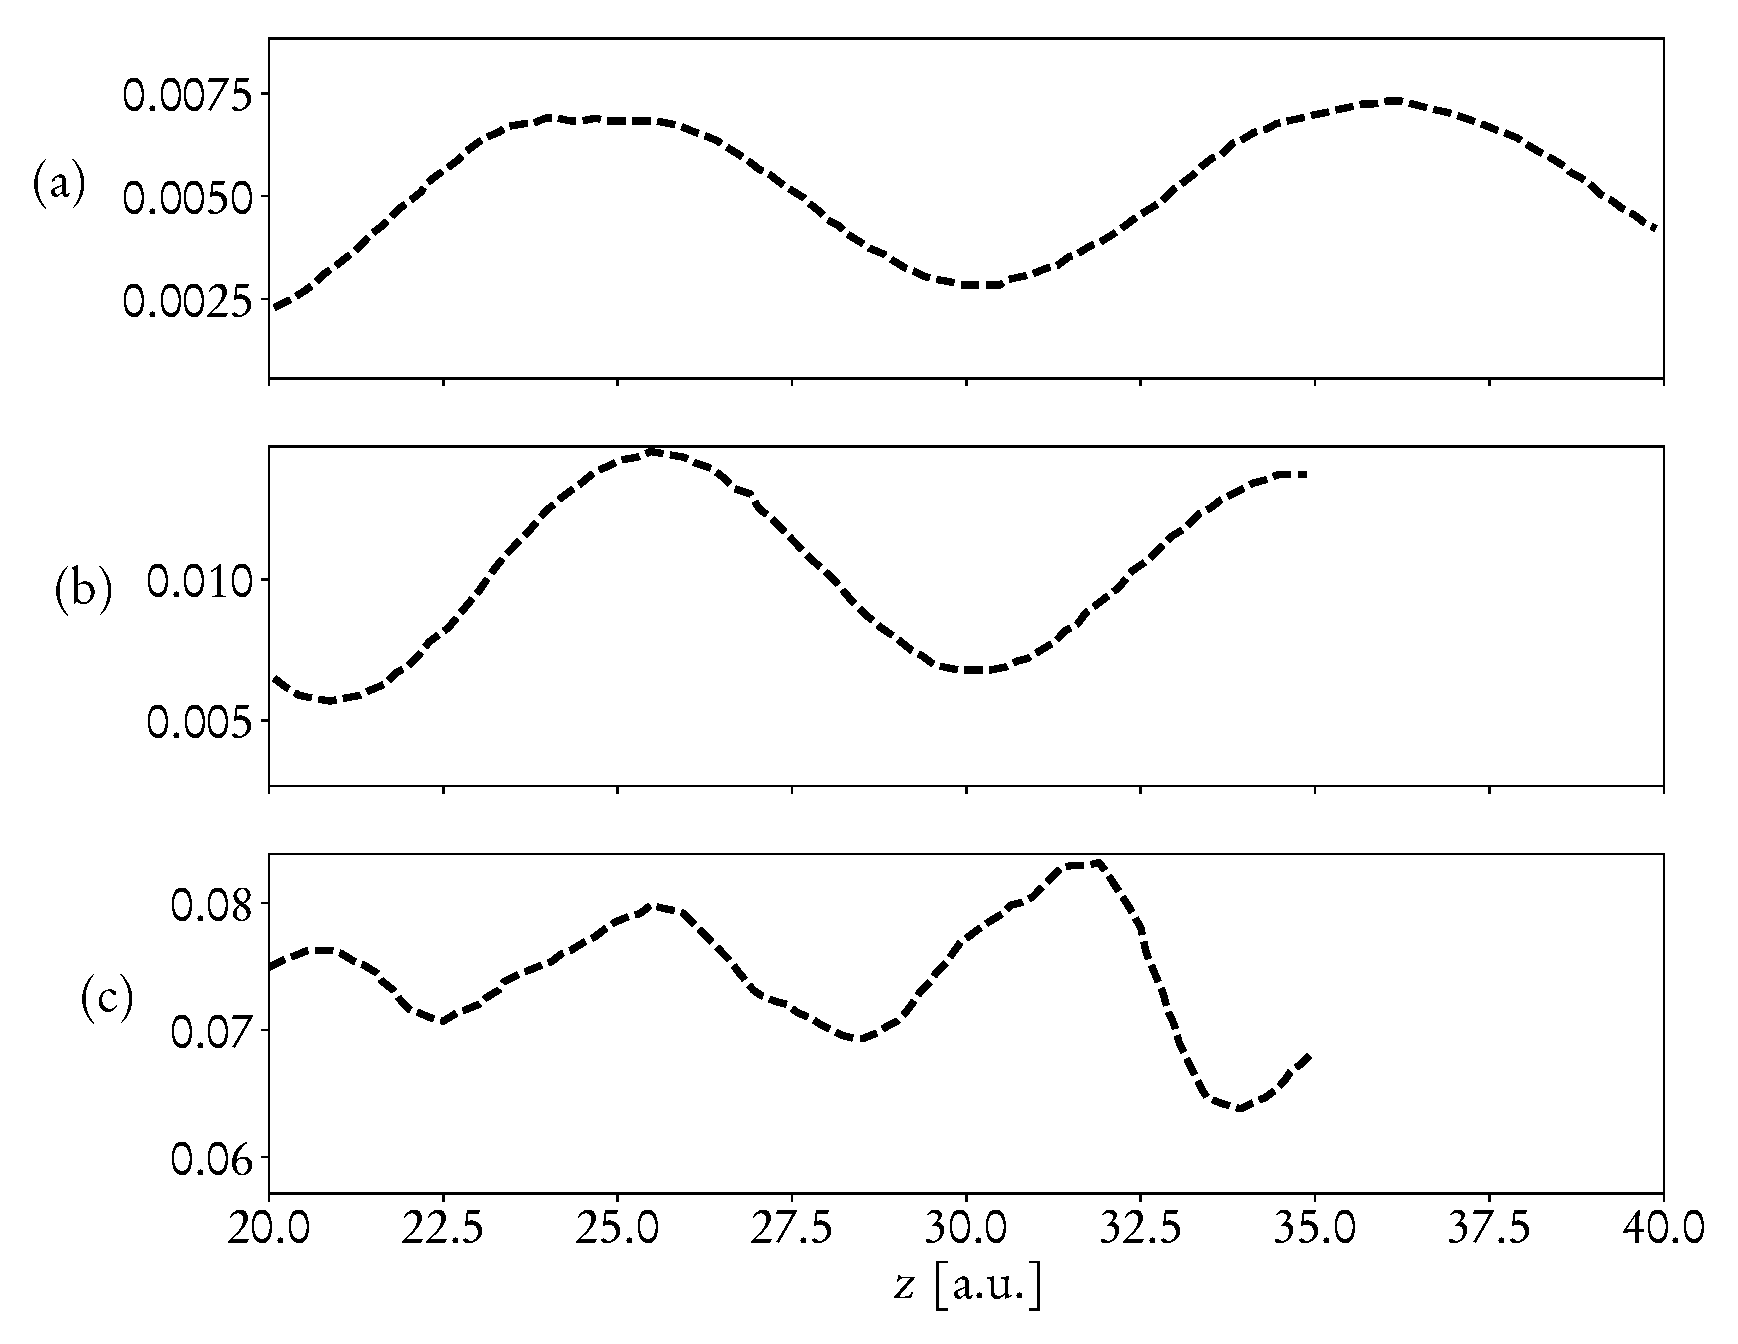
\includegraphics[width = \linewidth]{./images/poz.eps}
            \caption[Probabilities as a function of nuclear separation.]{$p^{II}$ as a
                     function of $z$ an impact energy of 50~keV and impact parameter of 1~a.u.:
                     (a)~$p$-He, (b)~He\textsuperscript{2+}-He, (c)~$\bar{p}$-He. \label{fig:poz}}
         \end{minipage} \hspace{0.04\linewidth} %
         \begin{minipage}{.49\linewidth}
            
            \centering
            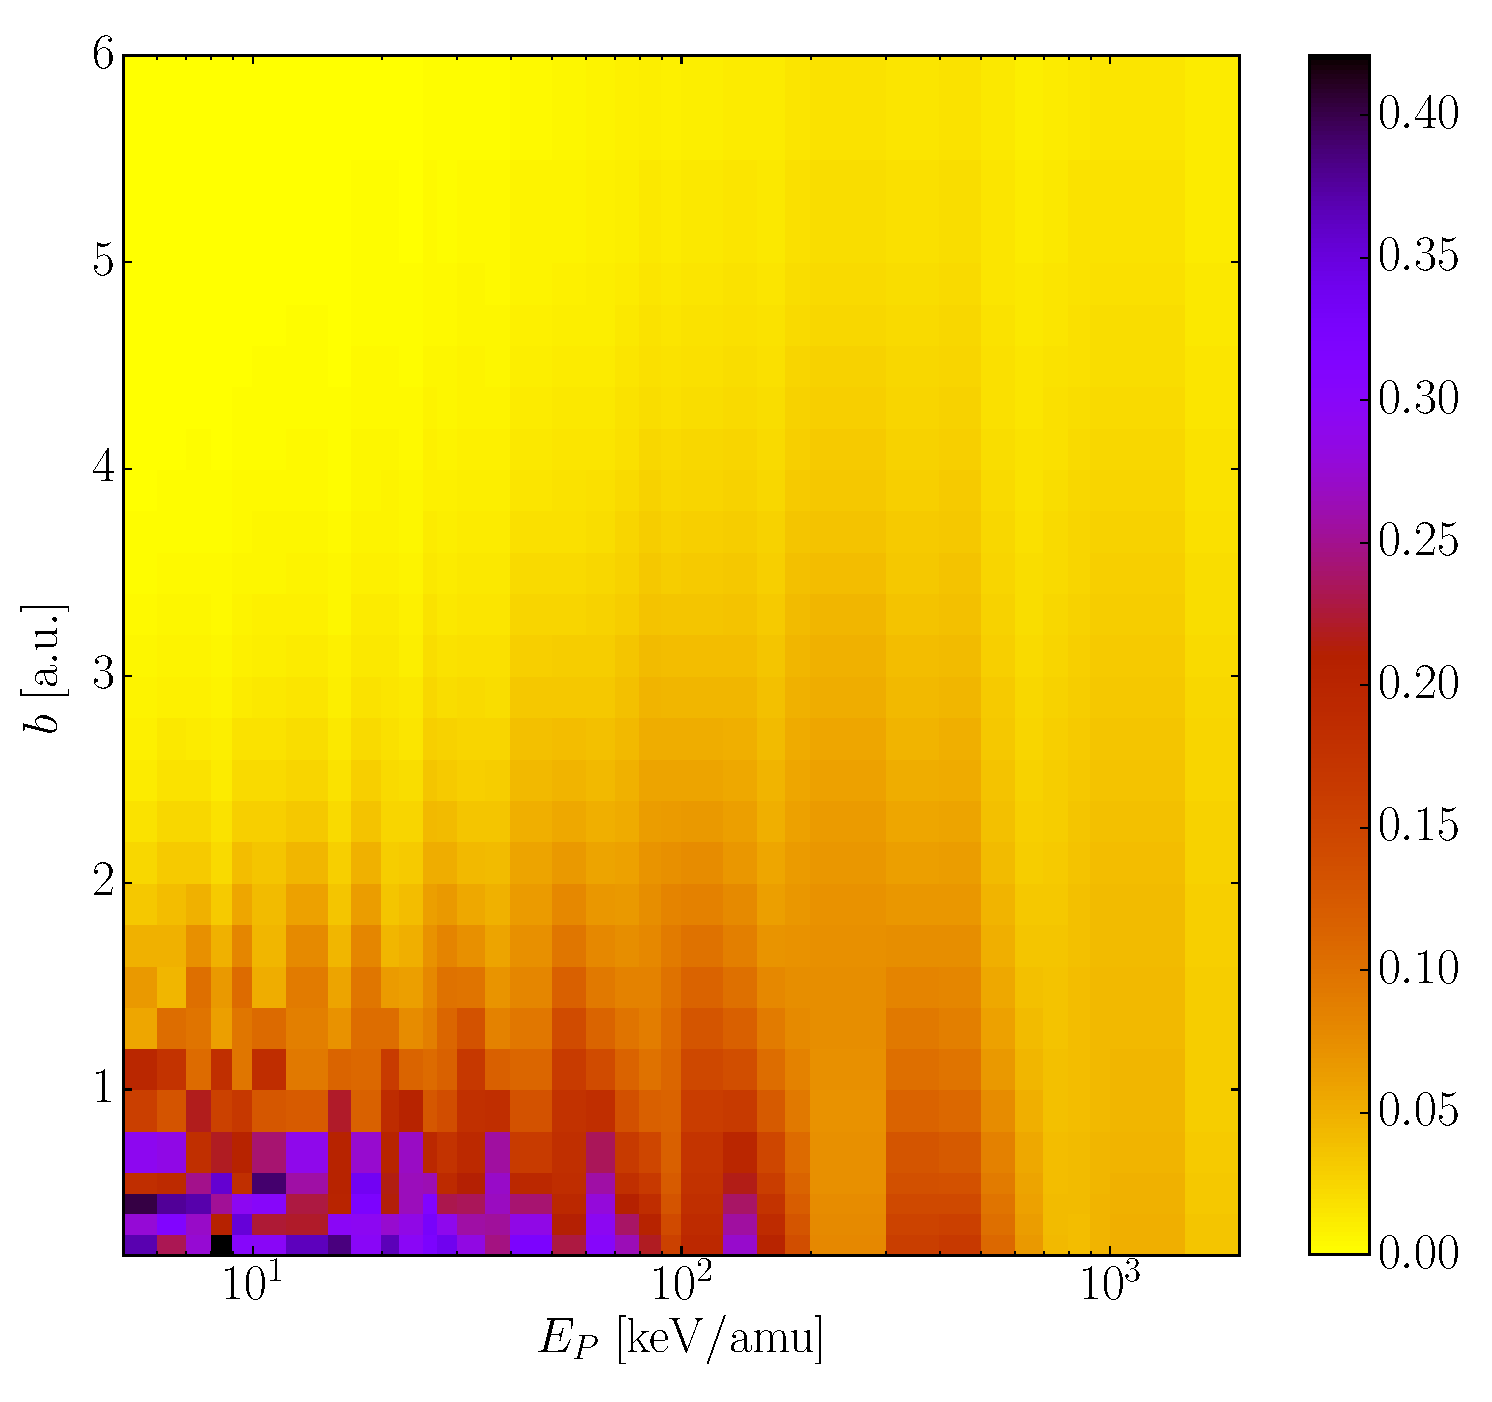
\includegraphics[width = \linewidth]{./images/dendiff.eps}
            \caption[Density difference]
                   {$\left| n_A\left(t_f \right) - n\left(t_f\right)\right|_1$ for the antiproton
                    helium collision system. \label{fig:l1}}
         \end{minipage}
      \end{figure}

      As has been discussed in previous works, for example~\cite{microresp,pbarhe}, fluctuations in the
      density persist after the collision process has completed if the Kohn-Sham potential is explicitly
      density dependent. Due to this fact the values of observables must be averaged over some range of
      $t_f$. The added complexity of the proton-helium collision system compared to that for
      antiproton-helium restricts the range through which the calculations may be run. Due to this fact
      an insufficient range of $t_f$ is available for averaging to produce a curve as smooth as in the
      $\bar{p}$-He system (see Fig.~\ref{fig:he++}). More explicitly, letting $z_f = V t_f$ be the final
      target-projectile separation for impact velocity $V$, $\bar{p}$-He collisions may be run to a
      final separation of 45~a.u., whereas $p$-He collisions run to a maximum inter-centre distance of
      around 35~a.u.
      
      Figure~\ref{fig:poz}, which depicts the values of $p^{II}$ as a function of $z$ for a prototypical
      choice of impact energy and parameter, makes these more apparent. Also of note is that the
      variances increase by about a factor of two between each of the collision systems.

      We can get a sense of how well the adiabatic density approximates the true time-dependent density
      at $t_f$ by considering there separation in function space between them. Owing to the fact that
      one-particle densities are necessarily $L^1$ functions (i.e.\ integrable functions) it is most
      natural to use the metric induced by the $L^1$-norm defined for any
      $f \in L^1\left(\mathbb{R}\right)$ by
      %
      \begin{equation} \label{eq:l1rorm}
         \left| f \right|_1 = \int \mathrm{d}^3 r \; \left| f(\mathbf{r}) \right|
      \end{equation}
      %
      for measuring this distance.
      
      Fig.~\ref{fig:l1} displays $\left| n(t_f) - n_A(t_f) \right|_1$, the
      difference between the adiabatic ($n_A$) and exact ($n$) densities at the final time $t_f$ for the
      antiproton-helium system\footnote{All integrals were performed with the aid of the \textsc{cuba} 
      numerical integration package~\cite{cuba}.}. While it is possible to perform such an analysis for
      the $p$-He system as well added complications brought on by having to deal with a two centred
      system make it much more difficult to produce and analyze such data. Intuitively one would expect
      that the difference between the two densities would scale with the single-particle probability
      $p_T$. This belief is supported by the easily derived relation 
      %
      \begin{equation} \label{eq:diff-bound}
         \left| n(t_f) - n_A(t_f) \right|_1 \leq 4 p_T.
      \end{equation}
      %
      While Fig.~\ref{fig:p-ic} (which will be discussed in next section) demonstrates monotonic
      increase in $p_T = 1 - p$ with increasing impact parameter, a general trend for all impact
      energies, Fig.~\ref{fig:l1} contains additional structures. Also of note is the minimum that
      appears along the impact energy axis between 200 and 300~keV/amu. These unexpected features must
      be attributed to the fact that $n_A$ contains only trivial angular dependence which makes a proper
      description of excitation and partial removal of electronic density impossible. This provides
      indications of the limitations of the \textsc{wb} model.

   \end{section}

   \begin{section}{Results \label{sec:phe2p-res}}

      In the following subsections we present several plots of total cross sections for a variety of
      collision processes. Given an outcome probability $p_\mathrm{outcome}$ the total cross section
      associated with this probability is determined according to
      %
      \begin{equation} \label{eq:tcs}
         \sigma_\mathrm{outcome} = \int \mathrm{d}^2 b \, p_\mathrm{outcome} (\mathbf{b})
         = 2 \pi \int^\infty_0 \mathrm{d}b \; b \, p_\mathrm{outcome} (b).
      \end{equation}
   
      We will refer to our results using the acronyms \textsc{iem} and \textsc{wb} corresponding to
      probabilities calculated using Eq.~\eqref{eq:prob-iem} and Eq.~\eqref{eq:prob-ic} using the
      \textsc{wb} model respectively. In both cases the dynamics include the frozen \textsc{mchf}
      ground-state correlation potential.

      The figures presented below were generated with several criteria in mind. First, a minimal number
      of older calculations was selected with the aim of covering as much of the impact energy range as
      possible while avoiding over burdening the figures with multiple overlapping curves. Second, works
      chosen must be the product of calculations that go beyond an \textsc{iem} description of the
      collision process with preference given to fully correlated two-electron calculations. If one is
      interested in some of the calculations excluded from these comparisons there exist a plethora of
      independent electron, independent event, or related models~\cite{SLD-83, DMR-84, SLD-85, GM-86,
      CM-87, GM-87, JLF-89, DC-90, DC-91a, DC-91b, DG-91, SKG-91, SL-91, Kuang-92, MLC-93, CM-94,
      CSR-95, BDM-96, MBGH-97, McCartney-97, Mccartney-99, GAMRF-02, GFS-02, AMRF-04, BLMC-04, FRBJG-06,
      FJG-07, GIFK-08, ZK-09, G-11, LFG-11, GG-12a}, classical trajectory Monte Carlo
      calculations~\cite{ZM-85, OWM-86, MO-87, WO-88, MS-89, Cohen-96, TH-96, MMTH-02, DAKW-04, GEP-09},
      and other classical statistical models such as the Bohr-Lindhard model~\cite{DYC-08,Ding-12} for
      one to consider at their own leisure.

      \begin{subsection}{ \texorpdfstring{$\bar{p}$}{pbar}-He Vs. \texorpdfstring{$p$}{p}-He Collisions
                         \label{sec:pbarhe-res}}

         \begin{figure}[t]
            \centering
            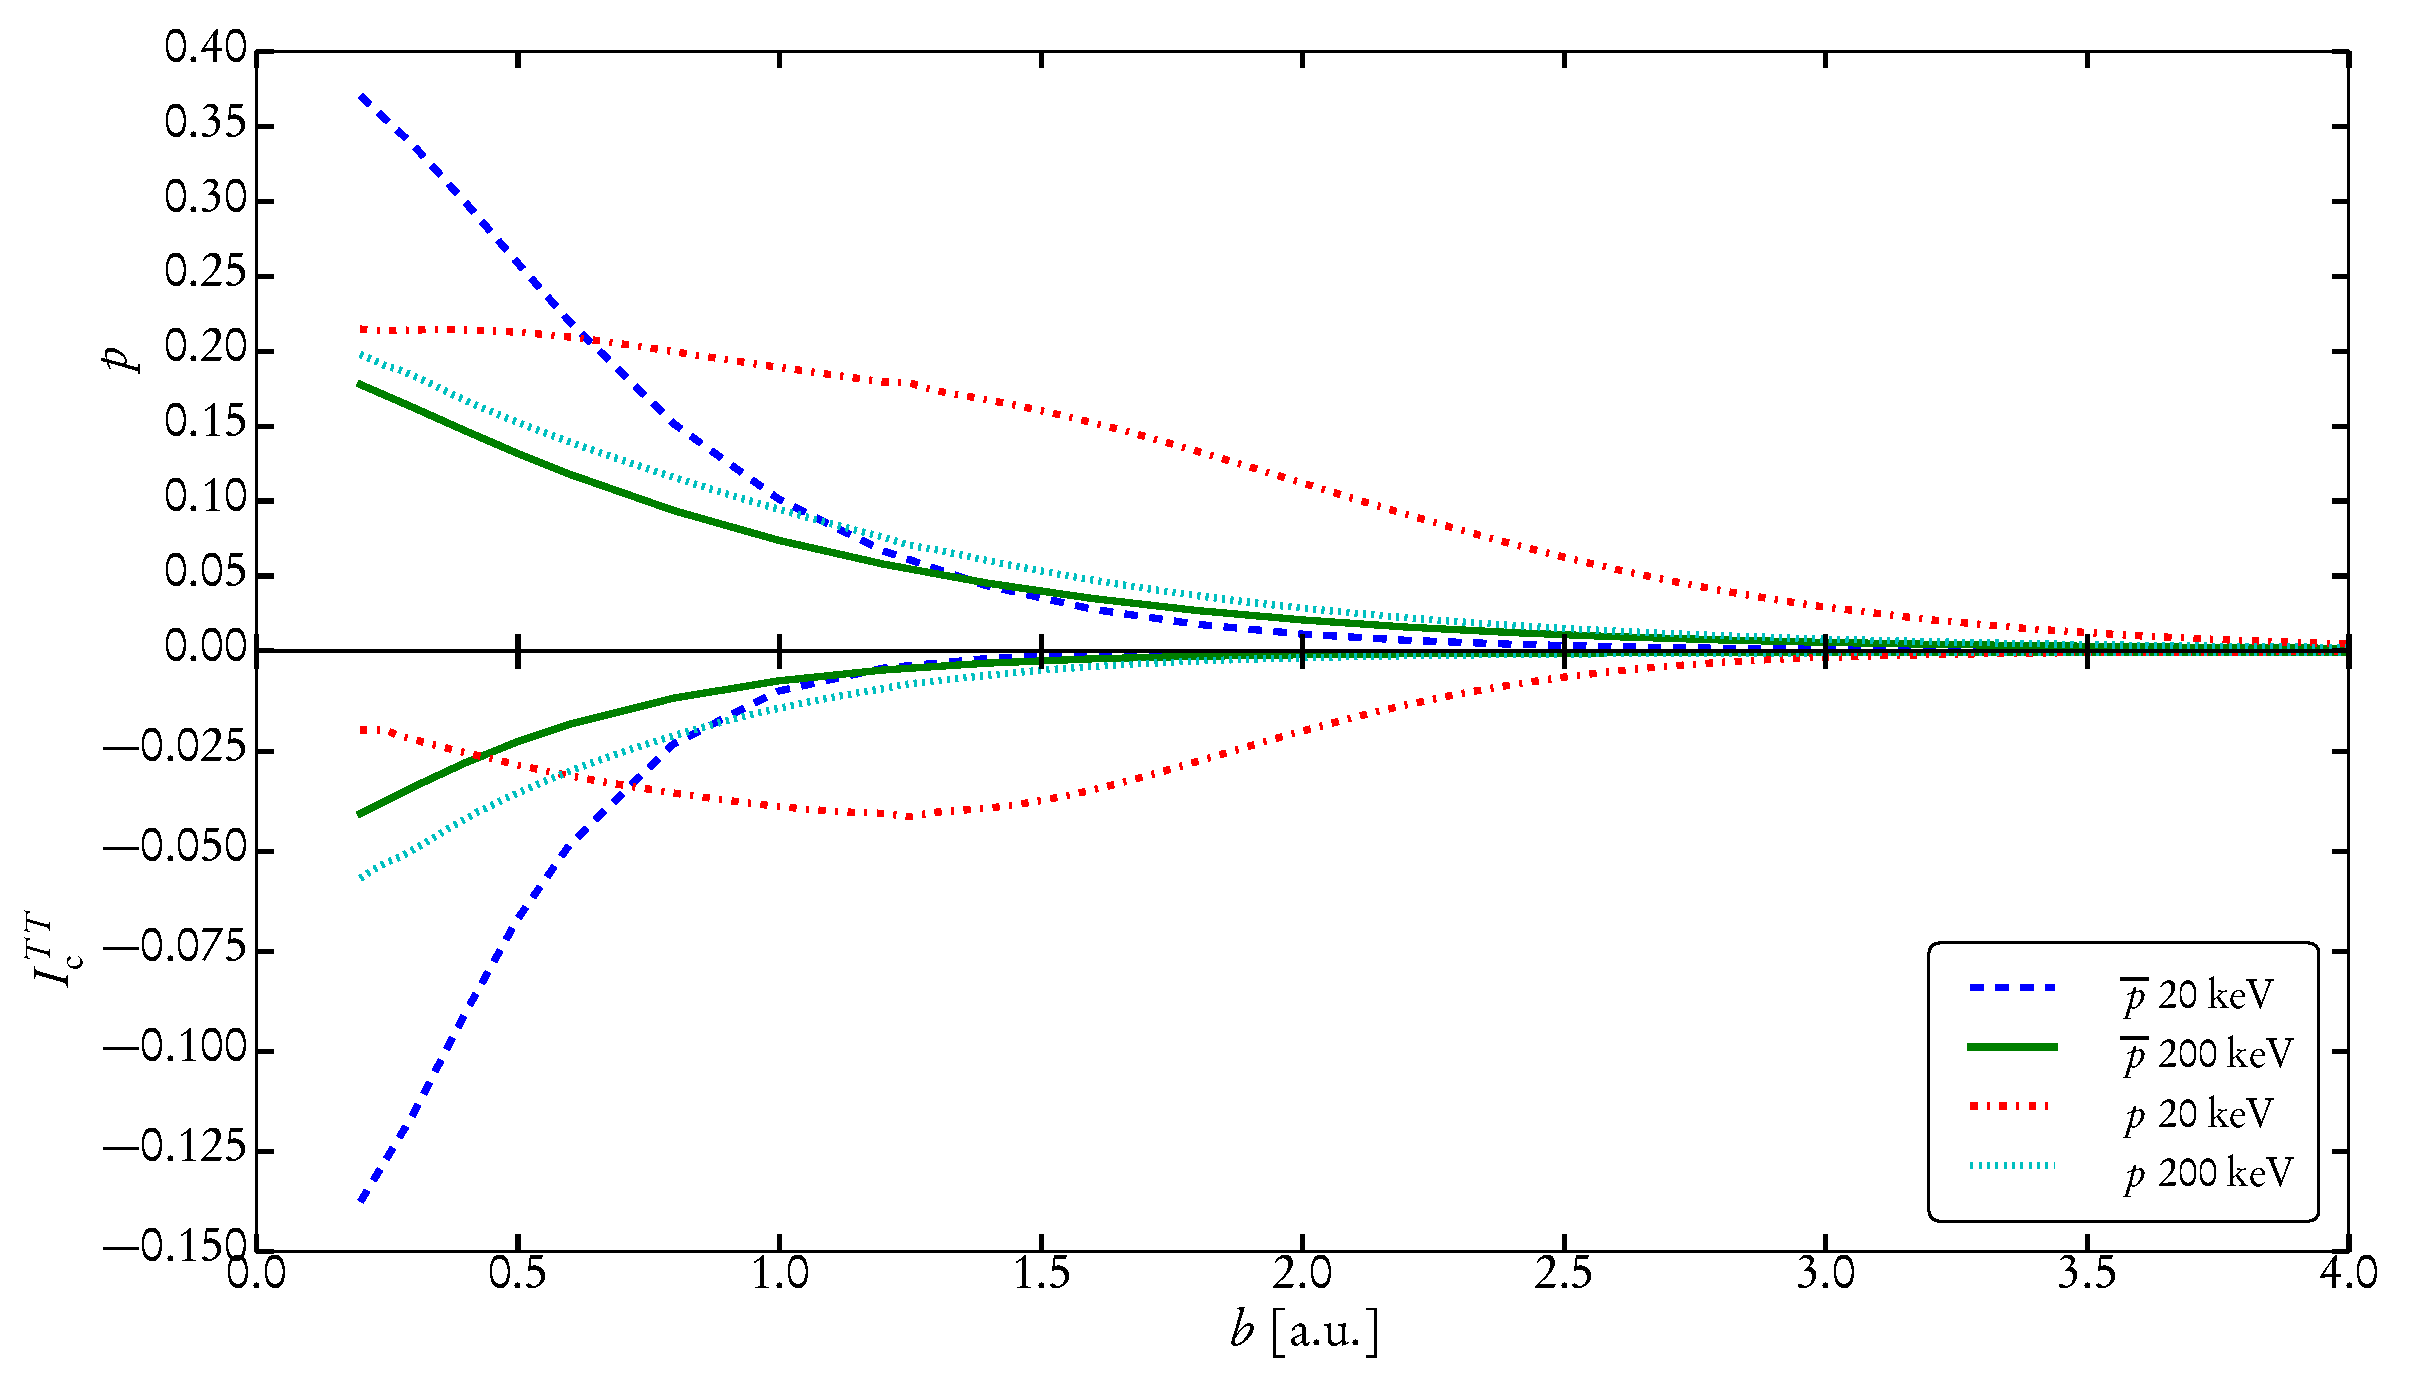
\includegraphics[width = 0.95 \linewidth]{./images/p-ic.eps}
            \caption[Single-particle removal and correlation integral]
                    {Single-particle removal probability, $p$, (upper pane) and
                     correlation integral, $I_\mathrm{c}^{TT}$, (lower pane) as functions of impact
                     parameter for antiprotons and protons incident on helium atoms at 20 and
                     200~keV/amu. \label{fig:p-ic}}
         \end{figure}

         \begin{figure}[t]
            \centering
            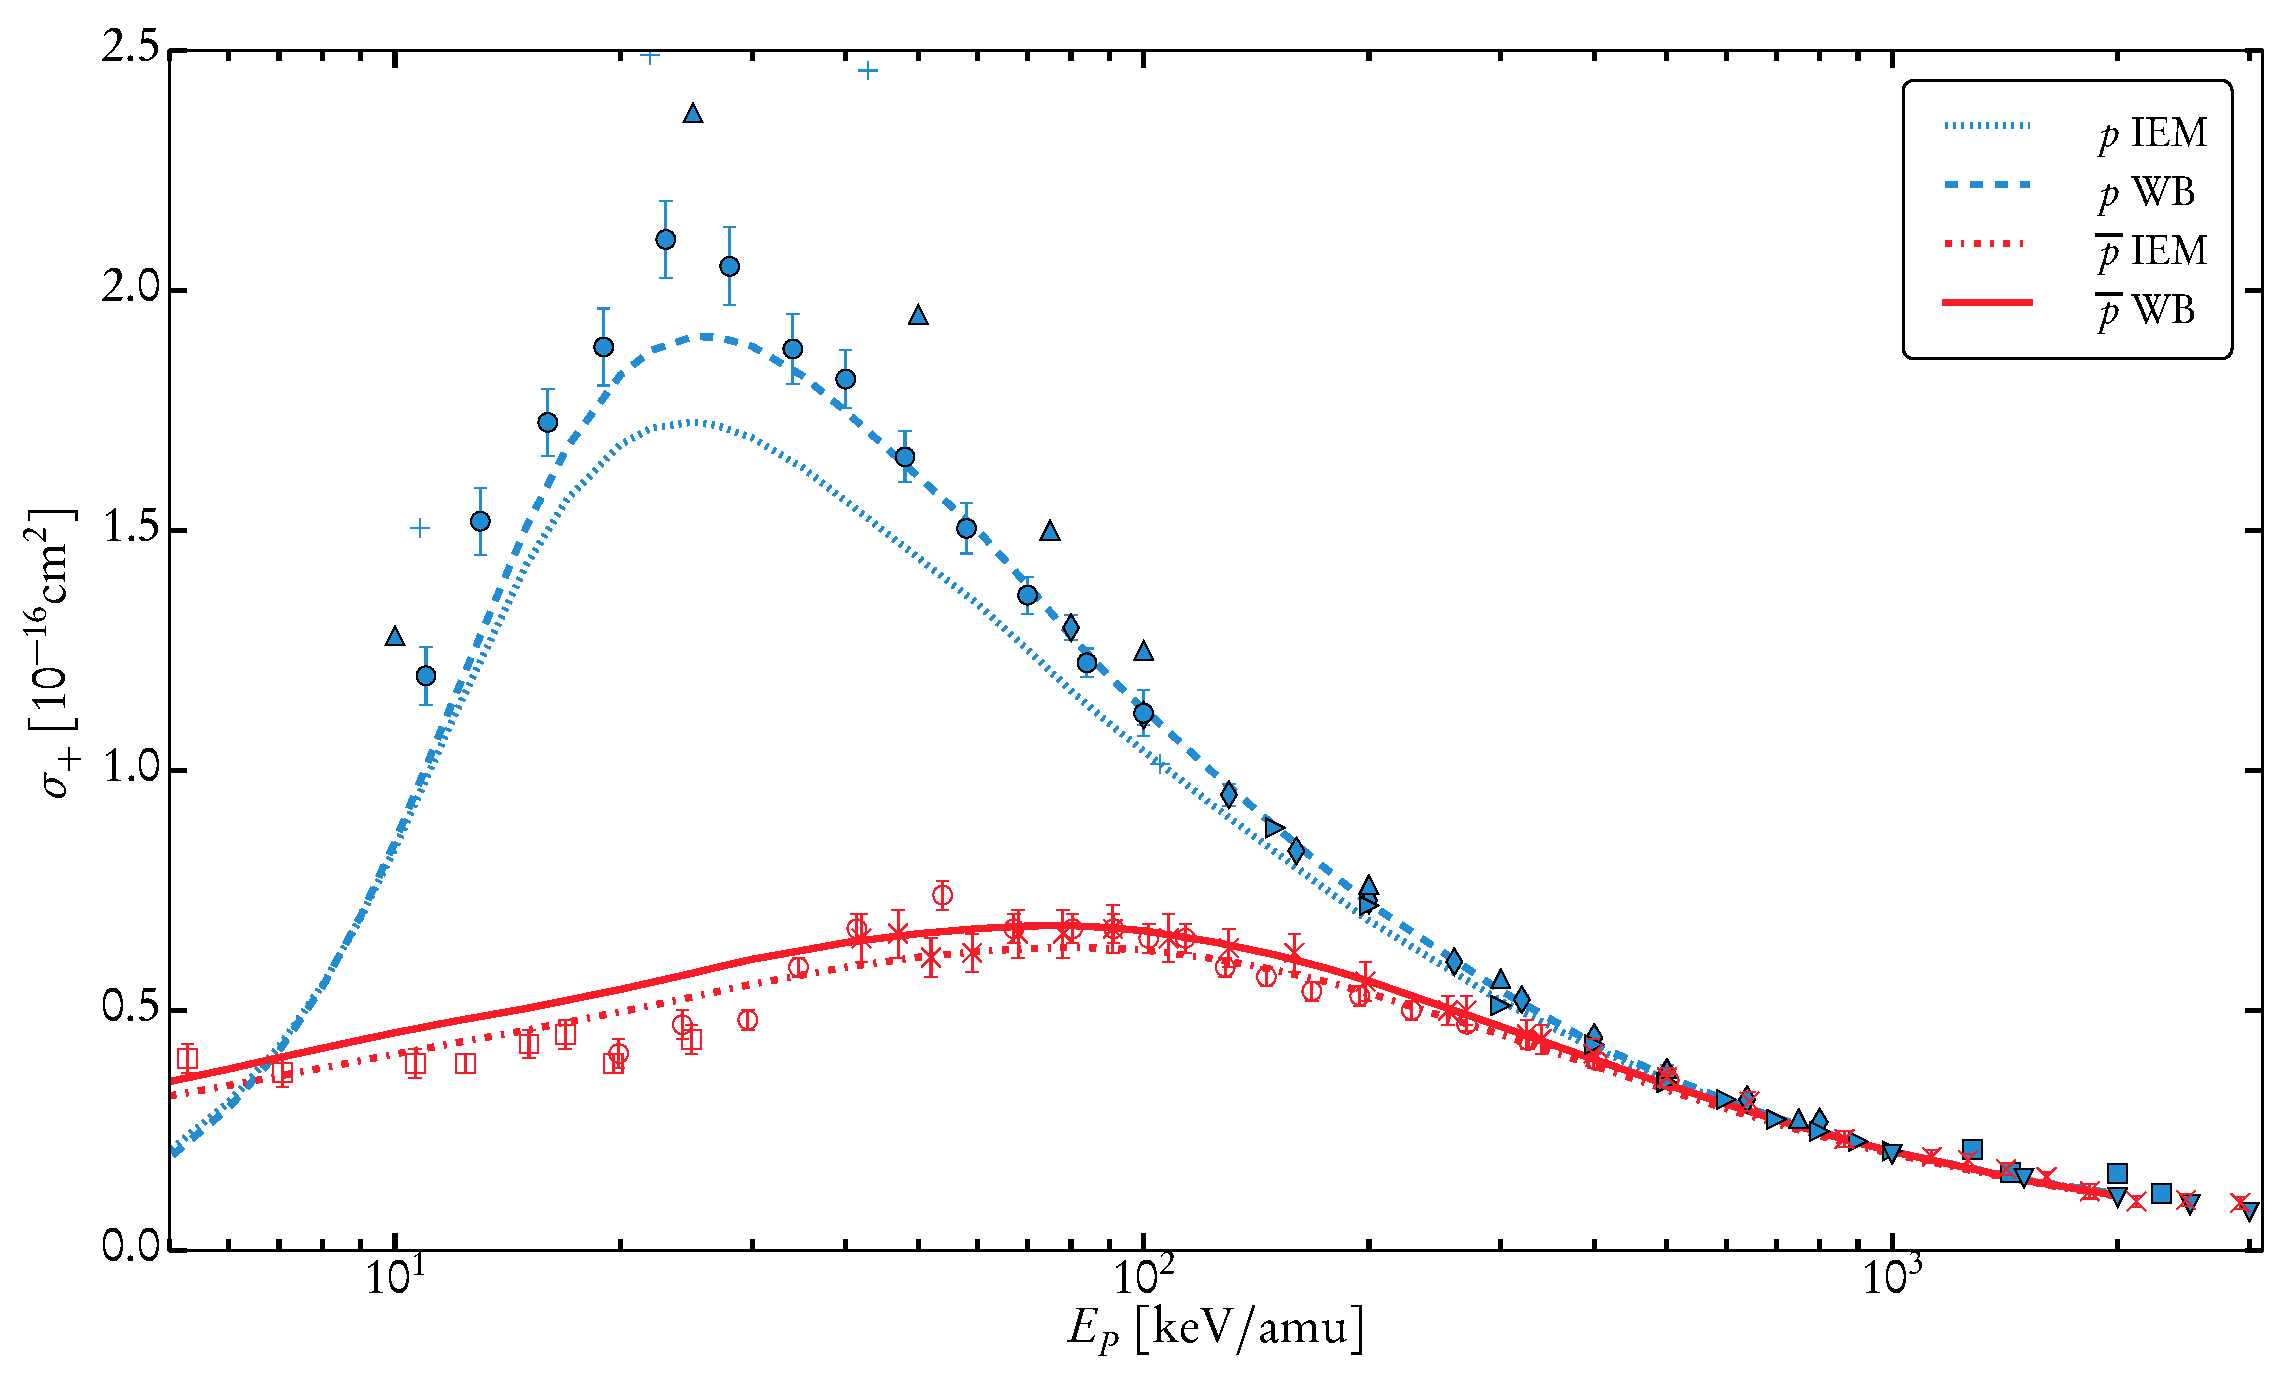
\includegraphics[width = 0.95 \linewidth]{./images/pbarhe/pbarhe-+.eps}
            \caption[Total cross section for one-electron removal from helium by protons and
                     antiprotons.]
                    {Total cross section for one-electron removal from helium by protons and
                     antiprotons. Protons: dotted \textsc{iem}, dashed \textsc{wb} (theory);
                     {\color{blue}{$\blacktriangle$}}~\cite{DTR84}, {\color{blue}{$+$}}~\cite{Sol62},
                     {\color{blue}{$\bullet$}}~\cite{SG89}, {\color{blue}{$\blacklozenge$}}~\cite{SG85},
                     {\color{blue}{$\blacktriangleright$}}~\cite{PM70},
                     {\color{blue}{$\blacktriangledown$}}~\cite{Wex64},
                     {\color{blue}{$\blacksquare$}}~\cite{KAH84} (experiment).
                     Antiprotons: dashed-dotted \textsc{iem}, solid \textsc{wb} (theory);
                     {\color{red}{$\Box$}}~\cite{KKT08}, {\color{red}{$\circ$}}~\cite{HKM94},
                     {\color{red}{$\times$}}~\cite{AHK90} (experiment). \label{fig:he+}}
         \end{figure}

         \begin{figure}[t]
            \centering
            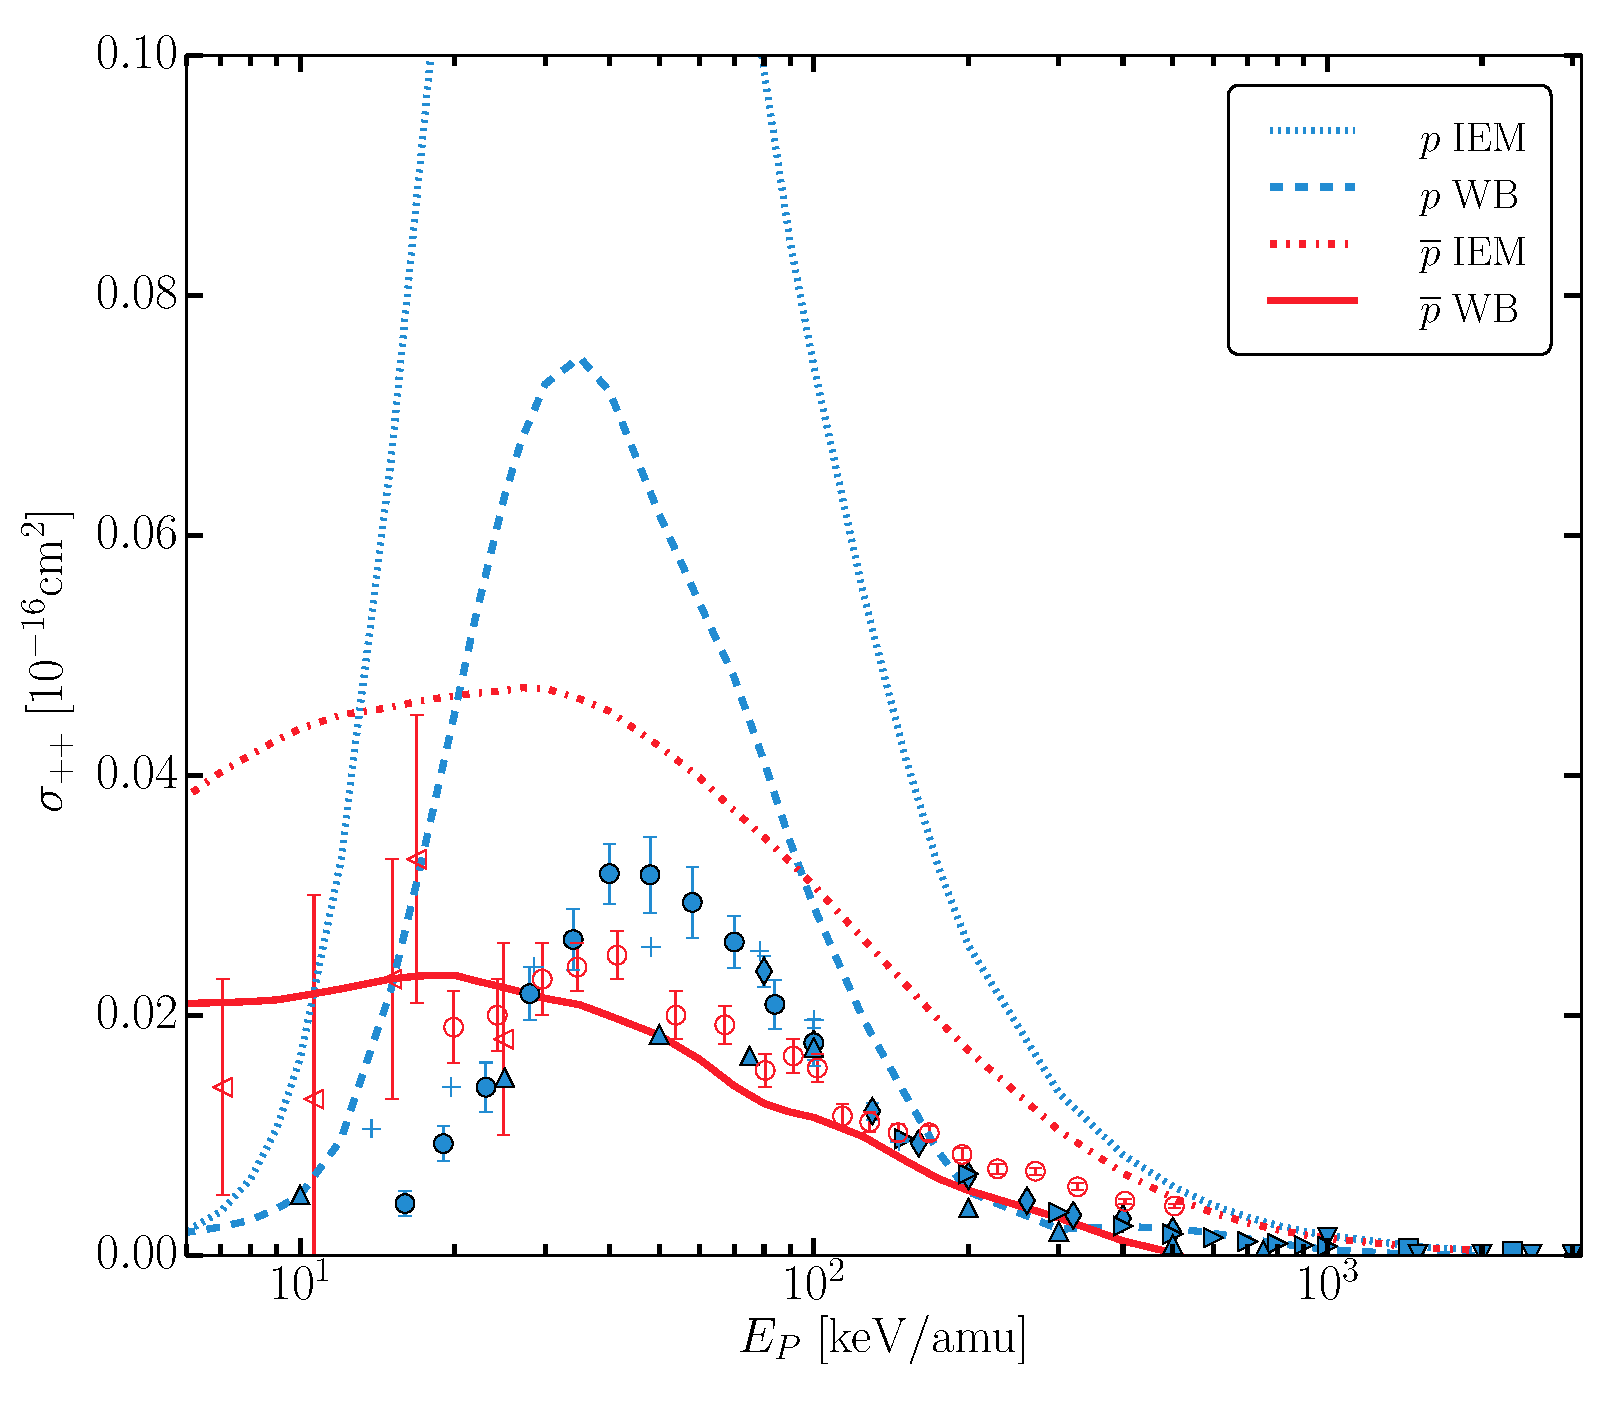
\includegraphics[width = 0.95 \linewidth]{./images/pbarhe/pbarhe-++.eps}
            \caption[Total cross section for two-electron removal from helium atoms as a function of
                     impact energy]
                    {Total cross section for two-electron removal from helium atoms as a function
                     of impact energy. Protons: dotted \textsc{iem}, dashed \textsc{wb} (theory);
                     {\color{blue}{$\blacktriangle$}}~\cite{DTR84}, {\color{blue}{$+$}}~\cite{Sol62},
                     {\color{blue}{$\bullet$}}~\cite{SG89},
                     {\color{blue}{$\blacklozenge$}}~\cite{SG85},
                    {\color{blue}{$\blacktriangleright$}}~\cite{PM70},
                    {\color{blue}{$\blacktriangledown$}}~\cite{Wex64},
                    {\color{blue}{$\blacksquare$}}~\cite{KAH84} (experiment).
                    Antiprotons: dashed-dotted \textsc{iem}, solid \textsc{wb} (theory);
                    {\color{red}{$\circ$}}~\cite{HKM94}, {\color{red}{$\triangleleft$}}~\cite{KKT09}
                       (experiment). \label{fig:he++}}
         \end{figure}

         We begin the analysis of results with a comparison of proton and antiproton collisions with
         helium. To facilitate juxtaposition we will consider the zero-, one-, and two-electron removal
         processes in aggregate. The probabilities for these outcomes are given respectively by
         %
         \begin{subequations} \label{eq:remove}
            \begin{equation} \label{eq:rem-0}
               p_0 = (1 - p)^2 + \tfrac{1}{2} I^{TT}_\mathrm{c} = p^{TT},
            \end{equation}
            %
            \begin{equation} \label{eq:rem-1}
               p_+ = 2 p (1-p) - I^{TT}_\mathrm{c} = p^{TI} + p^{TP},
            \end{equation}
            %
            \begin{equation} \label{eq:rem-2}
               p_{++} = p^2 + \tfrac{1}{2} I^{TT}_\mathrm{c} = p^{II} + p^{IP} + p^{PP},
            \end{equation}
         \end{subequations}
         %
         where the single-particle removal probability is given by
         %
         \begin{equation} \label{eq:p-rem}
            p = 1 - \tfrac{1}{2} \int_T \mathrm{d}^3 r \; n(\mathbf{r},t_f)
            = 1 - p_T = p_P + p_I.
         \end{equation}
         %
         For the $\bar{p}$-He system these are simply the probabilities presented in
         Eq.~\eqref{eq:prob-pbarhe} making this choice of observables ideal for contrasting with the
         $p$-He system.

         Presented in Fig.~\ref{fig:p-ic} are the single-particle removal probability and
         $I^{TT}_\mathrm{c}$ for both the proton and antiproton collision systems at 20 and 200~keV/amu
         as functions of the impact parameter. The correlation integral is always negative, decaying to
         zero in increasingly distant collisions as electron removal becomes less likely. This means
         that it provides a blanket enhancement to one-electron removal processes
         [cf.\ Eq.~\eqref{eq:rem-1}]. 

         At 200~keV/amu the results for both $p$ and $I^{TT}_\mathrm{c}$ become similar; at lower
         energies (i.e., 20~keV/amu) there are significant differences for proton and antiproton
         collisions. In this range the single-removal probability for antiprotons decays swiftly with
         rising impact parameter. On the other hand, the single-particle removal probability in low
         energy proton-helium collisions remains appreciable over a much larger range. Such impact
         parameter profiles are a signature of electron capture which is the dominant electron removal
         process at lower impact energies. This behaviour is mirrored by that of $I^{TT}_\mathrm{c}$.

         A final feature of note is the spike in both antiproton curves at low impact parameter. In this
         region the antiproton passes through the charge density of the helium atom. Such close
         approaches result in destabilization of the electron binding and very efficient
         ionization~\cite{pbarhe-rev}

         Figures~\ref{fig:he+} and~\ref{fig:he++} present the total cross sections for one- and
         two-electron removal as functions of impact energy. These plots compare only the current
         proton-helium collision results to an updated version (denser impact energy grid and larger
         range of averaging as described in Sec.~\ref{sec:phe2p-det}) of the antiproton-helium results
         of~\cite{pbarhe} and to experimental data. For a comparison with other theoretical work
         see~\cite{pbarhe} and~\cite{new-pbarhe} ($\bar{p}$-He) and Sec.~\ref{sec:phe-res} ($p$-He).
 
         For one-electron removal, Fig.~\ref{fig:he+}, the \textsc{wb} model provides an increase for
         both protons and antiprotons over the \textsc{iem} except at higher energies where the
         correlation integral tends to be small in magnitude as indicated by Fig.~\ref{fig:p-ic}. In the
         case of proton-helium collisions this increase is an obvious improvement. The spread of the
         experimental data for antiproton-helium collisions makes it difficult to ascertain whether the
         enhancement in the cross section is preferable.
 
         The two-electron removal cross sections, Fig.~\ref{fig:he++}, for both proton and antiproton
         collisions are reduced significantly by the \textsc{wb} model. These reductions represent a
         clear improvement in either case. While the antiproton results are in fair agreement with
         experiment through the entire range explored the proton-helium results still differ notably
         below impact energies of 100~keV/amu. This is an indication that the \textsc{wb} model begins
         to display problems as capture becomes more important. These issues will be discussed in
         greater detail in the proceeding subsections.

      \end{subsection}

      \begin{subsection}{\texorpdfstring{$p$}{p}-He Collisions \label{sec:phe-res}}

         \begin{figure}[t]
            \centering
            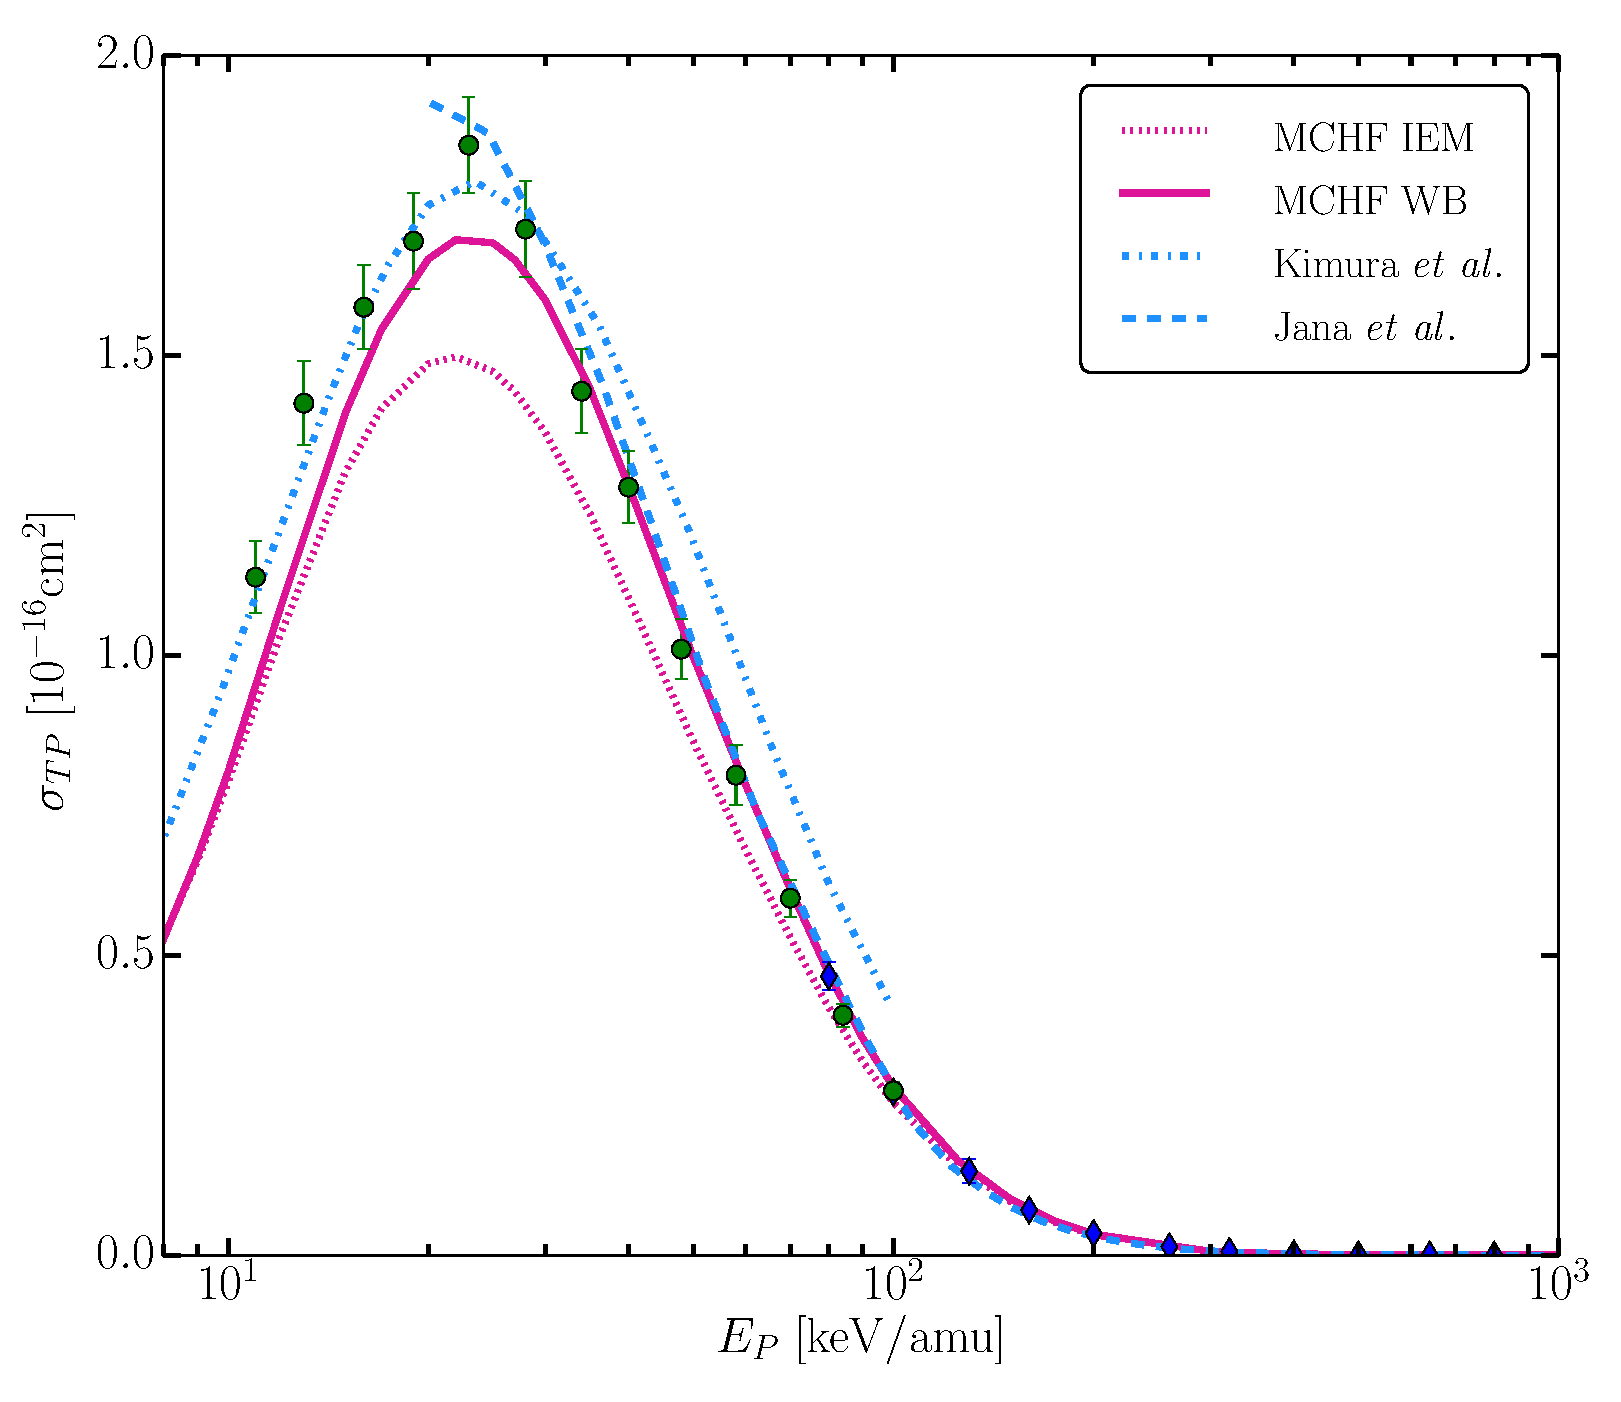
\includegraphics[width = 0.95 \linewidth]{./images/phe/phe-TP.eps}
            \caption[Total cross section for single capture in proton-helium collisions.]
                    {Total cross section for single capture in proton-helium collisions.
                     Theoretical results: \textsc{ao-mo} model of Kimura et al.~\cite{KL-86} and
                     \textsc{dw-4b} (post form) of Jana et al.~\cite{JMP-15}. Experimental Data:
                     {\color{OliveGreen}{$\bullet$}}~\cite{SG89} and
                     {\color{blue}{$\blacklozenge$}}~\cite{SG85}. \label{fig:phe-tp}}
         \end{figure}

         \begin{figure}[t]
            \centering
            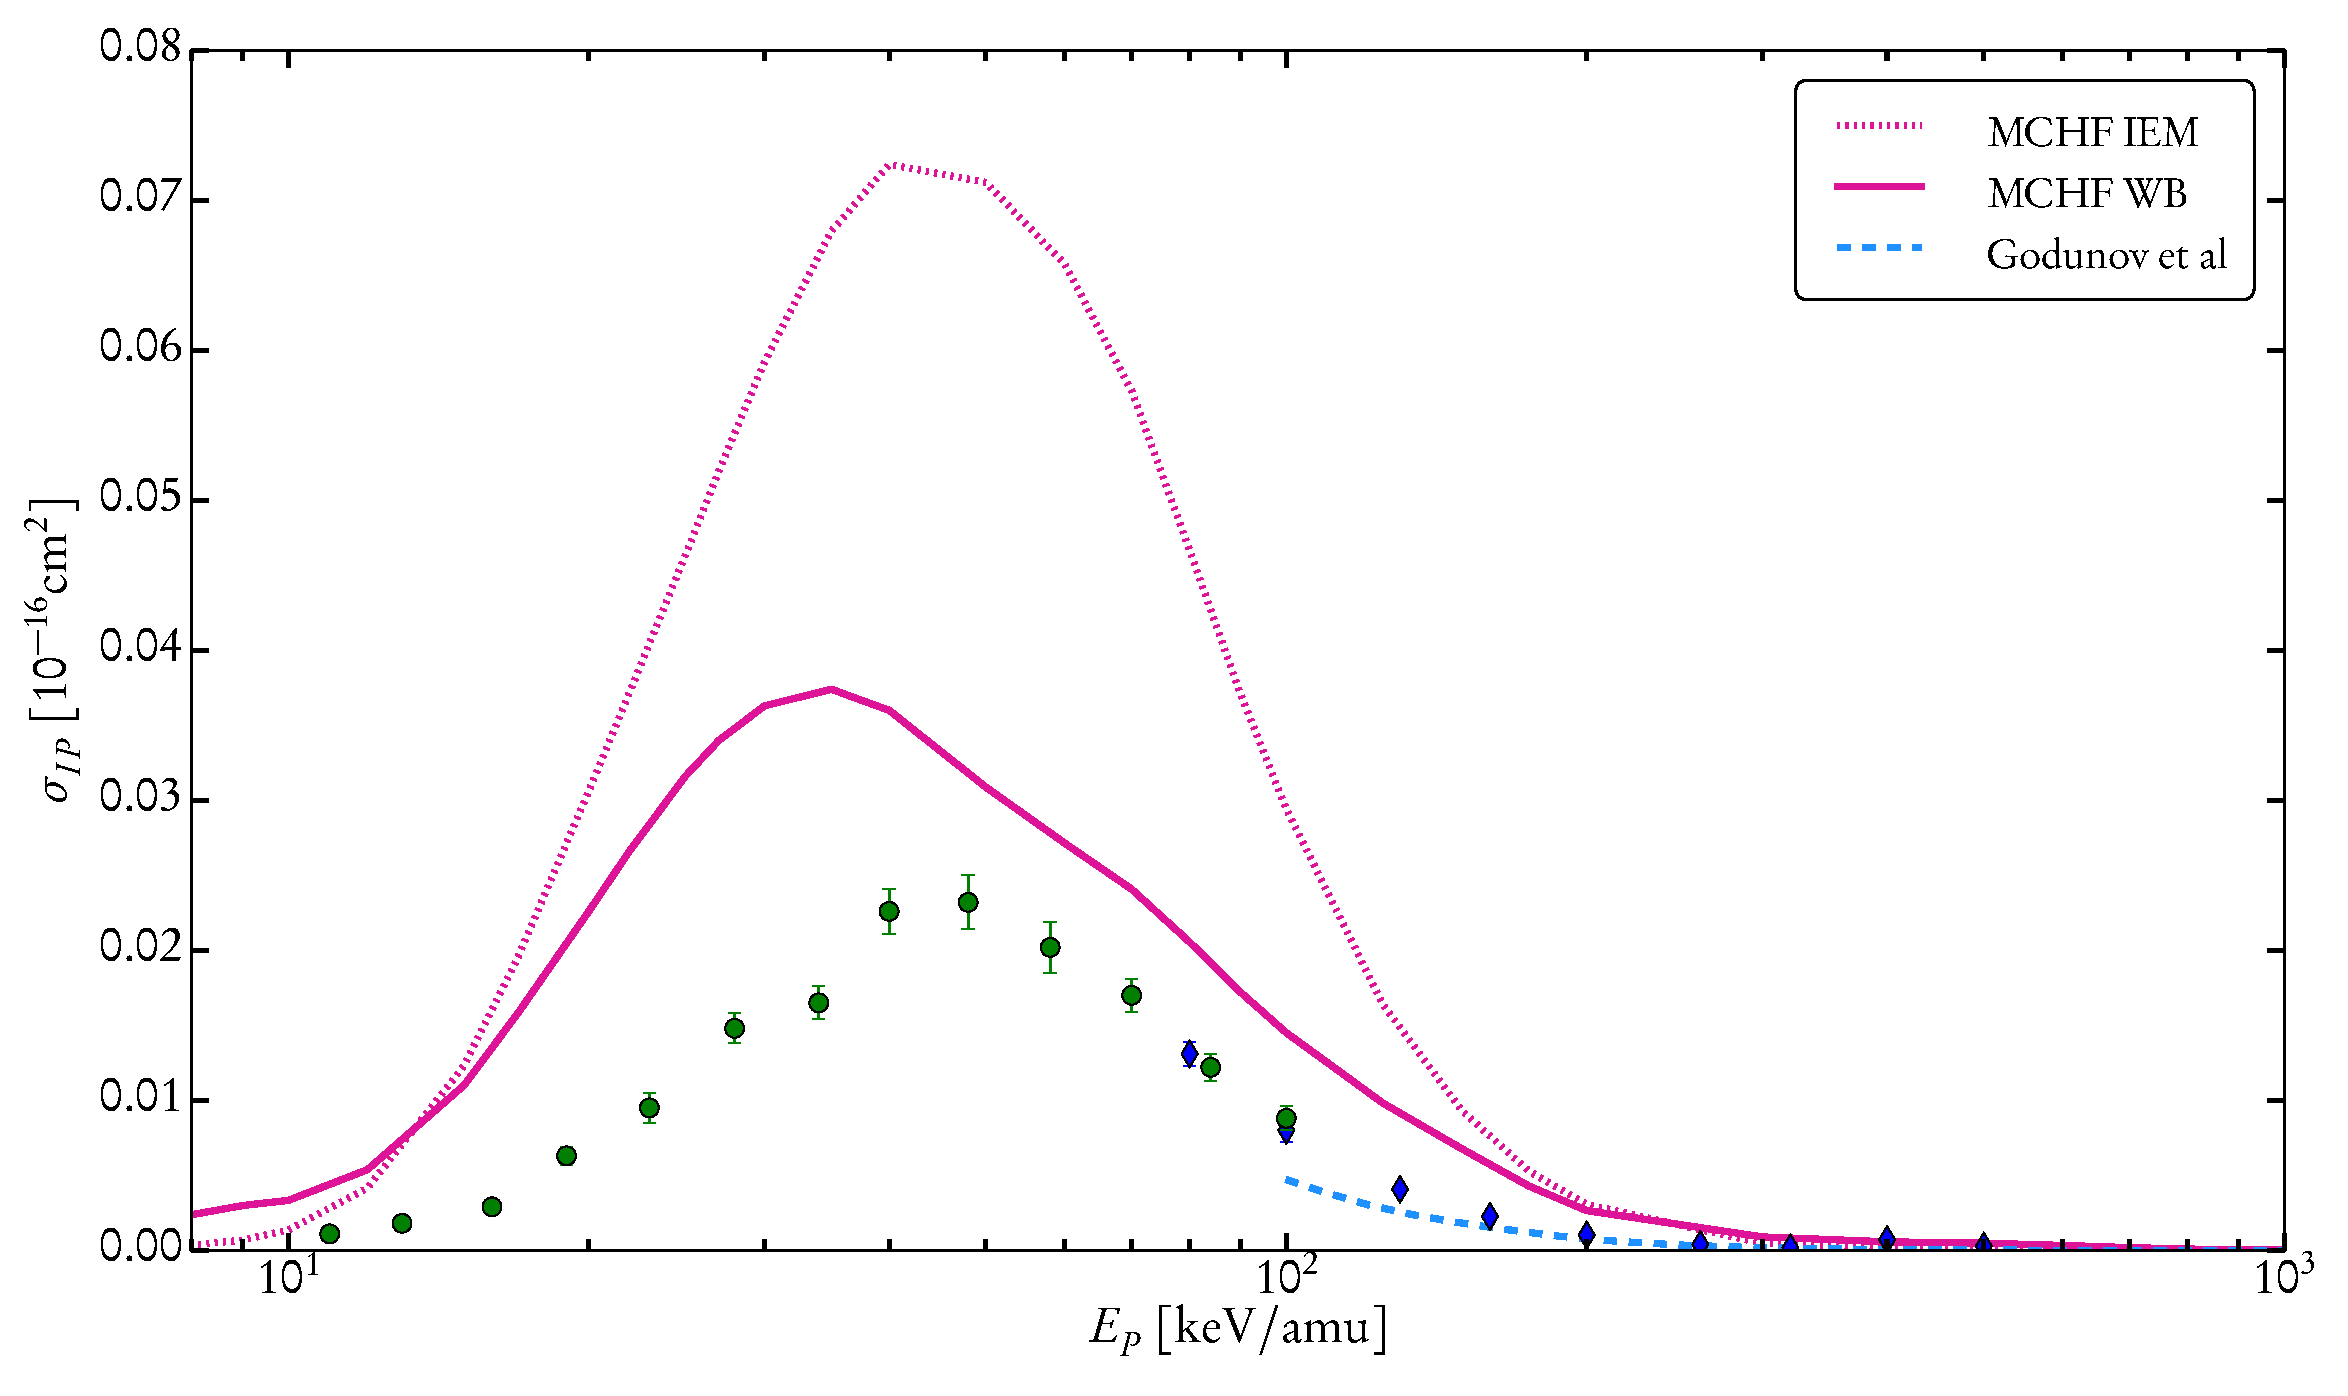
\includegraphics[width = 0.95 \linewidth]{./images/phe/phe-IP.eps}
            \caption[Total cross section for transfer ionization in proton-helium collisions.]
                    {Total cross section for transfer ionization in proton-helium collisions.
                     Theoretical results: Second order Born approximation of Godunov
                     et al.~\cite{Godunov-06}. Experimental data:
                     {\color{OliveGreen}{$\bullet$}}~\cite{SG89} and
                     {\color{blue}{$\blacklozenge$}}~\cite{SG85}. \label{fig:phe-ip}}
         \end{figure}

         \begin{figure}[t] 
            \centering
            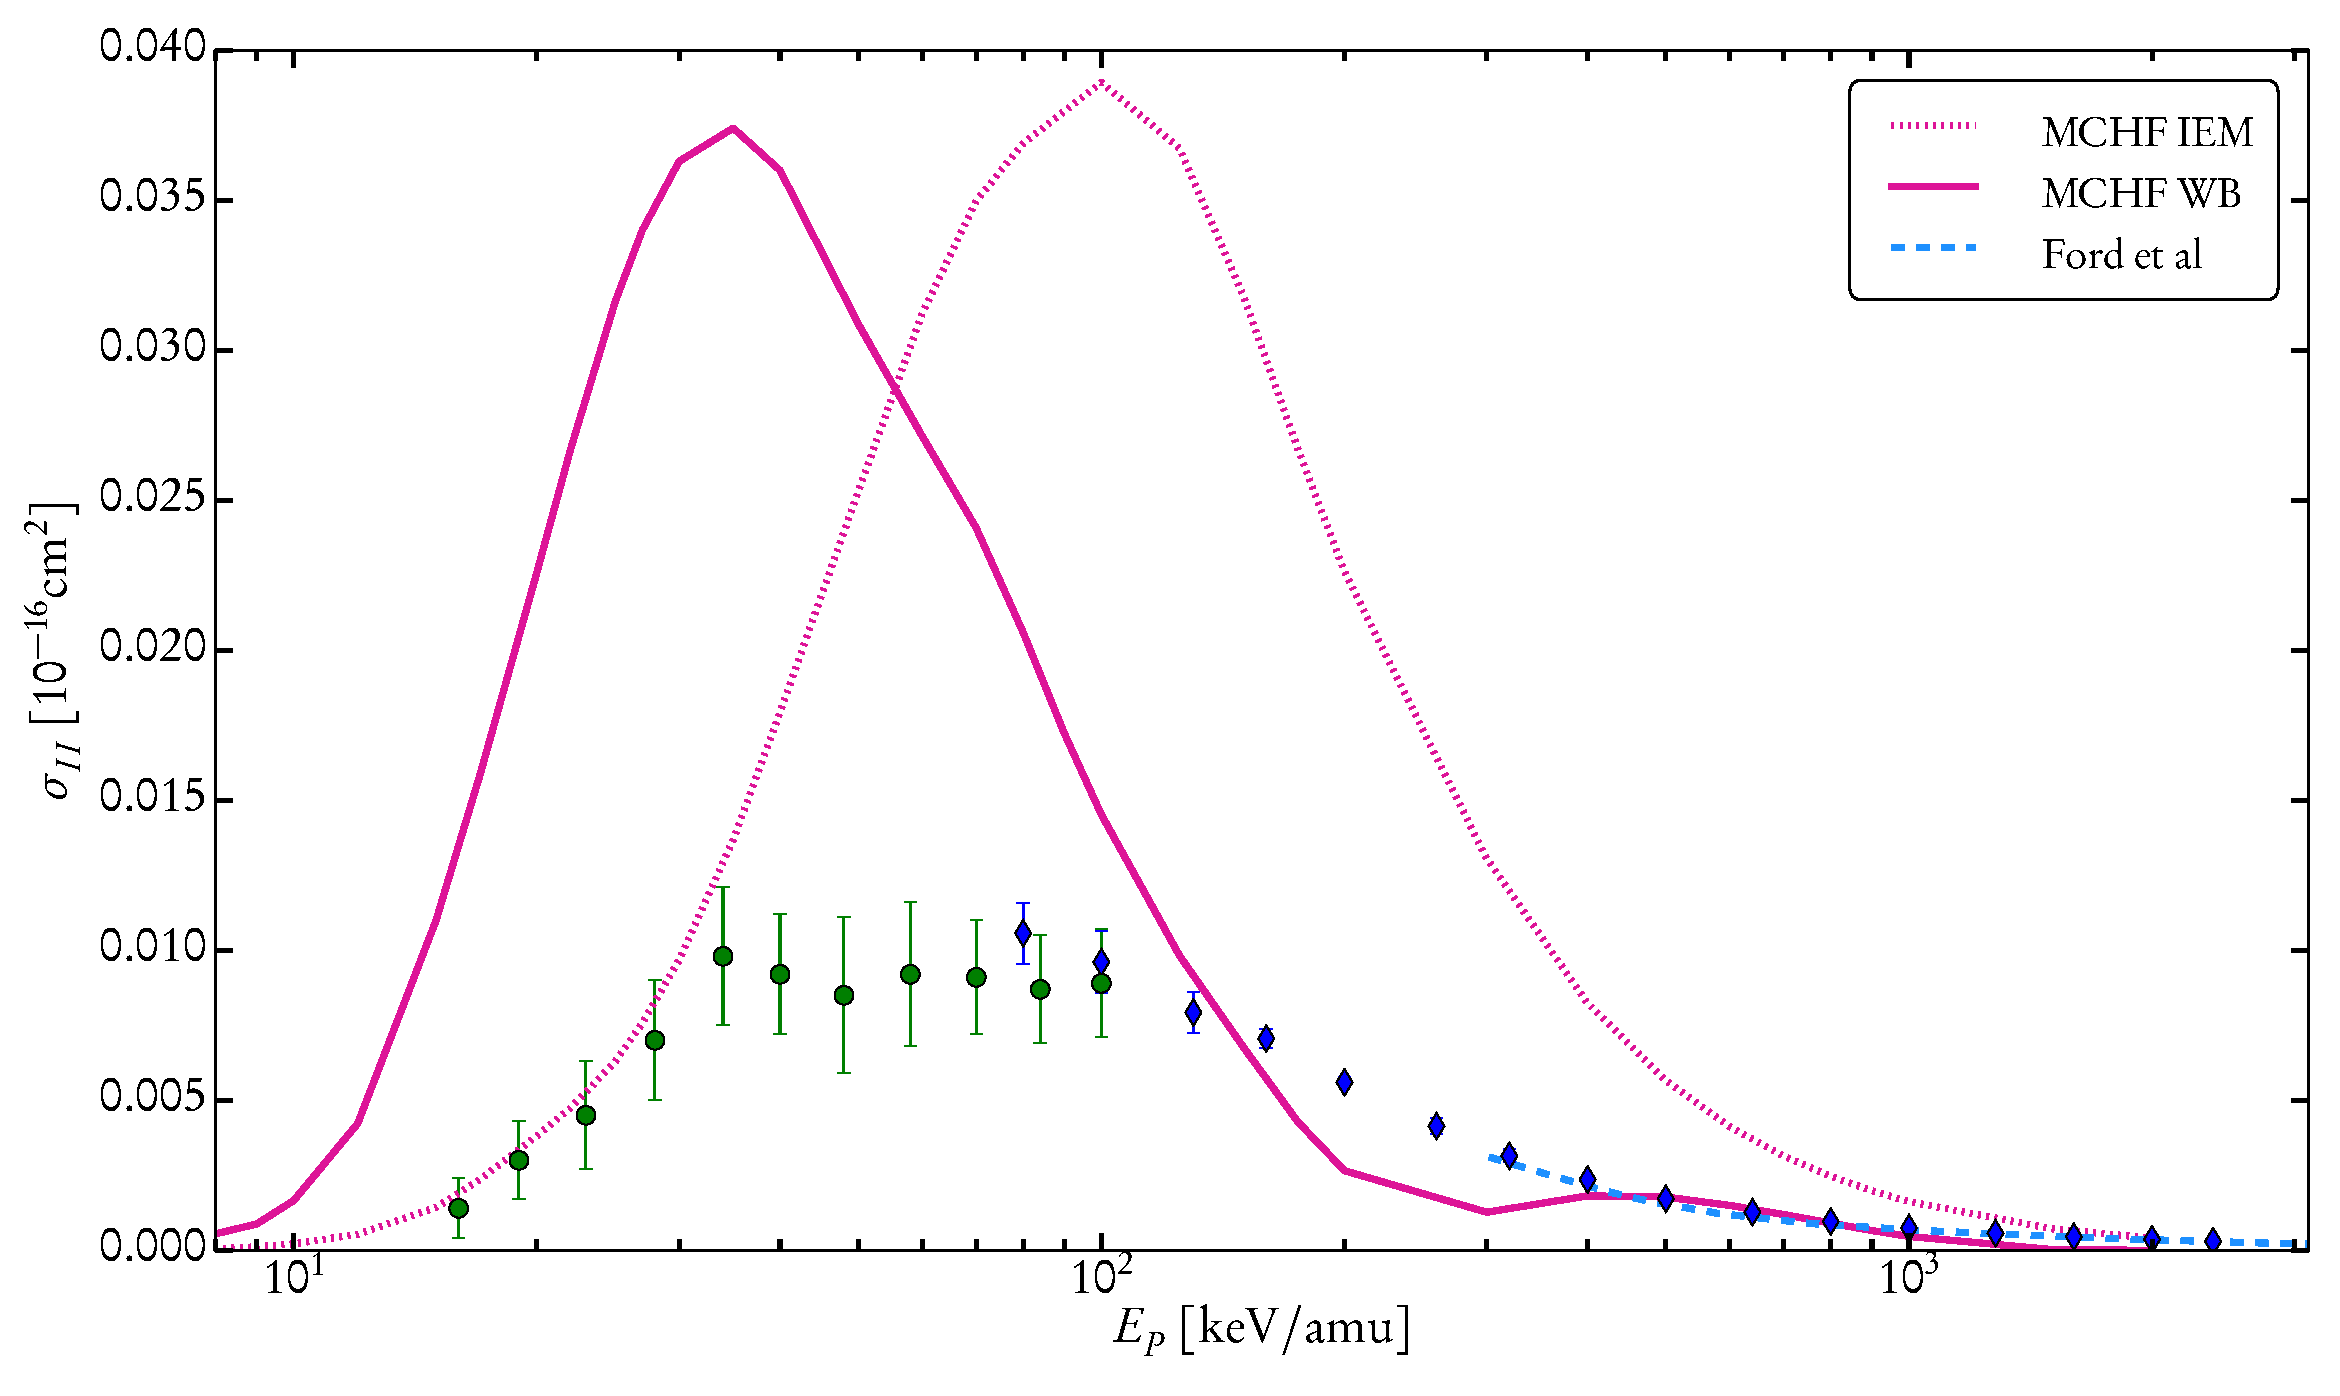
\includegraphics[width = 0.95 \linewidth]{./images/phe/phe-II.eps}
            \caption[Total cross section for double ionization of helium by proton impact.]
                    {Total cross section for double ionization of helium by proton impact.
                     Theoretical results: \textsc{fim} of Ford et al.~\cite{FR-94}.
                     Experimental data: {\color{OliveGreen}{$\bullet$}}~\cite{SG89} and
                     {\color{blue}{$\blacklozenge$}}~\cite{SG85}. \label{fig:phe-ii}}
         \end{figure}

         \begin{figure}[t] 
            \centering
            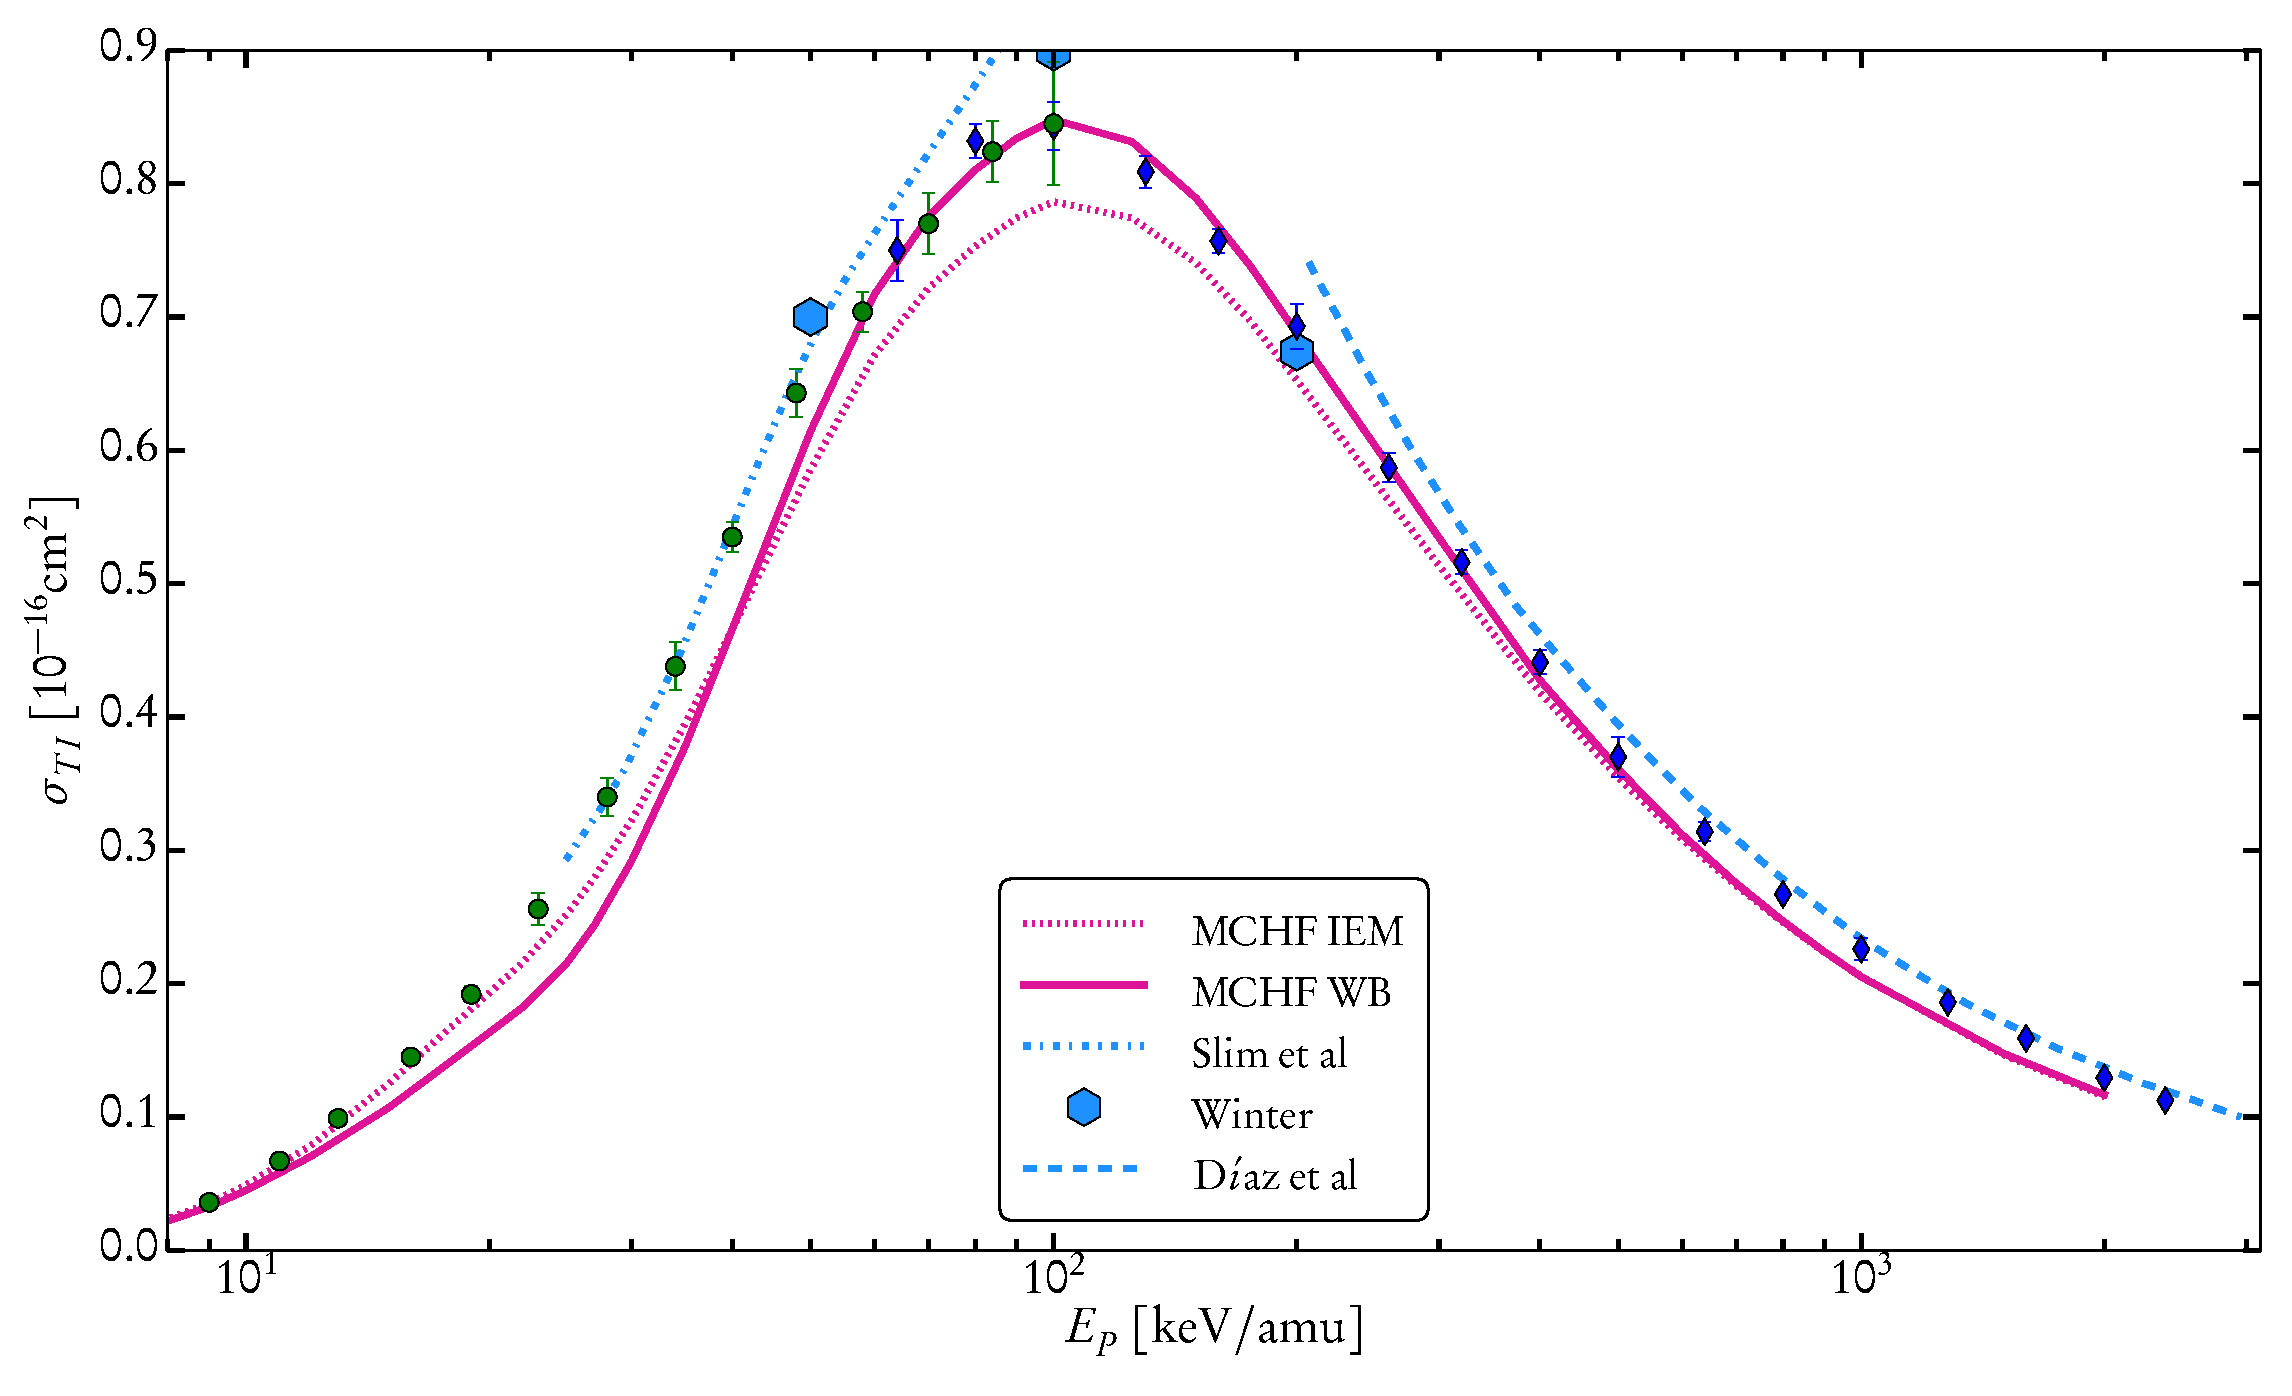
\includegraphics[width = 0.95 \linewidth]{./images/phe/phe-TI.eps}
            \caption[Total cross section for single ionization of helium by proton impact.]
                    {Total cross section for single ionization of helium by proton impact.
                     Theoretical results: Slim et al.~\cite{SHBF-91},
                     Winter~\cite{Winter-91}, D\'{i}az et al.~\cite{DMS-00}
                     Experimental data: {\color{OliveGreen}{$\bullet$}}~\cite{SG89} and
                     {\color{blue}{$\blacklozenge$}}~\cite{SG85}. \label{fig:phe-ti}}
         \end{figure}

         Total cross sections for the various ionization and capture processes described by
         Eqs.~\eqref{eq:prob-ic} and~\eqref{eq:prob-iem} for both the \textsc{wb} model and the
         \textsc{iem} are presented in Figs.~\ref{fig:phe-tp}--\ref{fig:phe-ti}. These results are
         compared to experiment as well as a selection of previous theoretical studies of $p$-He
         collisions that do account for electron correlation effects.

         We will begin the discussion of these results by considering double capture. For our
         proton-helium collision calculations the single-particle capture probability, $p_P$, never
         rises above 1/2. Using Eqs.~\eqref{eq:n1a} and~\eqref{eq:p2a} in Eq.~\eqref{eq:ic} (i.e.\
         applying the \textsc{wb} model) it follows that $I^{PP}_\mathrm{c} = -2 {p_P}^2$, which implies
         that $p_{PP} \equiv 0$. Due to the triviality of this result no plot has been displayed. The
         \textsc{iem} so amplifies the double capture cross section that the \textsc{wb} model can be
         considered in better agreement with experiment even though it is zero for all impact energies
         and perceived as an improvement over \textsc{iem}.

         Similar to double capture single-capture, Fig.~\ref{fig:phe-tp}, only depends on one
         correlation integral. The \textsc{iem} provides fair agreement with the experimental data
         except that it underestimates the peak. This problem is corrected by the \textsc{wb} model
         which is in good agreement with experiment through most of the impact energy range considered.
         This fact helps to justify the model used for $I^{TP}_\mathrm{c}$ in Eq.~\eqref{eq:ictp} as
         single capture is expressed as the \textsc{iem} result plus a correction coming solely from
         $I^{TP}_\mathrm{c}$ [cf.\ Eq.~\eqref{eq:ptp-ic}]. Also presented in Fig.~\ref{fig:phe-tp} are
         the atomic orbital (\textsc{ao}) molecular orbital (\textsc{mo}) matching results of Kimura et
         al.~\cite{KL-86} and the post form, which includes explicit dynamic correlation contributions,
         of the four-body distorted-wave (\textsc{dw-4b}) results of Jana et al.~\cite{JMP-15}. It
         should be noted that what Jana et al.\ call dynamic correlation while not identical to
         \textsc{tddft} dynamic correlation (a time-dependent correlation potential $v_\mathrm{c}$) is
         the analogue in two-electron calculations and ultimately both should describe the same effects.
         The \textsc{dw-4b} and \textsc{wb} models agree quite well above impact energies of 40~keV/amu.
         Below this they begin to deviate, with the \textsc{dw-4b} results remaining in better agreement
         with experiment (excluding the lower extremes of the data where the perturbative nature of the
         \textsc{dw-4b} model likely causes it to become less reliable). The opening of a gap between
         these two calculations coincides precisely with the increased role of dynamic correlation as
         impact energies decrease. This trend continues with the results of Kimura et al.\ throughout
         the remainder of the impact energy range. The discrepancy between the \textsc{ao-mo} results
         and the other calculations for energies above the peak is likely due to the dominance of the
         \textsc{mo} over the \textsc{ao} in the analysis~\cite{KL-86}. The result of this appears to be
         an overestimate of the coupling between centres leading to a slight overestimate of the cross
         section at large energies.

         Figure~\ref{fig:phe-ip} presents the results for transfer ionization. Once again the
         \textsc{wb} model offers an improvement over \textsc{iem} descriptions, lowering the cross
         section by as much as a factor of two. Even with this correction the \textsc{wb} still
         overestimates the data through the entire range. An unfortunate side effect of the model is a
         slight shift in the peak of the curve towards lower energies. The overestimation in this
         channel may be a result of the redistribution of probability which must occur with the double
         capture channel effectively closed by the \textsc{wb} model.
 
         Our \textsc{iem} and \textsc{wb} results are compared to the second-order Born approximation
         calculation of Godunov et al.~\cite{Godunov-06} (on- and off-shell contributions included). Few
         correlated transfer ionization calculations exist. As a result conclusions for the quality of
         correlation below 100~keV/amu are difficult. One additional calculation was performed by
         Belki\'{c} et al.~\cite{BM-11}. However, their data covers less of the desired impact
         energy range and was thus excluded from Fig.~\ref{fig:phe-ip}. Godunov et al.\ are
         consistently below both \textsc{iem} and \textsc{wb}. The fact that the \textsc{iem} falls
         slightly below the \textsc{wb} results above 200~keV/amu points to a problem with the
         \textsc{wb} calculations. In this range the difficulty of separating target and projectile (the
         projection problem) will naturally be emphasized as the relative errors due to the projection
         problem grow. It would seem that these issues are compounded when the density is forced through
         the additional machinery of the \textsc{wb} model. In this region it then becomes difficult to
         determine to what extent discrepancies are due to dynamic vs.\ functional correlation effects
         or issues of accuracy.

         Next we turn our attention to the results for double ionization in Fig.~\ref{fig:phe-ii}. The
         \textsc{wb} model improves results by reducing those of the \textsc{iem} at high energies.
         Agreement is lost as impact energy drops below 100~keV/amu. A close inspection of the double
         ionization result reveals that they are identical to those for transfer ionization in the
         approximate range 10--300~keV/amu.
 
         To understand what is causing this we must examine some of the ramifications of
         Eq.~\eqref{eq:ictp}. It can be shown that whenever $I^{TP}_\mathrm{c}$ is sandwiched between
         either $L_2$ and $U_4$ or $L_4$ and $U_2$ we have $p^{II} = p^{IP}$. As the former is true for
         the majority of contributing impact parameters for the energy range mentioned above we fall in
         a situation where double ionization and transfer ionization are forced to be equal.

         Another undesirable feature of the double ionization cross section is the dip below the
         experimental data between 100 and 400~keV/amu. As has been discussed in
         Sec.~\ref{sec:phe2p-det} the added complexity of the proton-helium collision system compared to
         that for antiproton-helium restricts the range through which the calculations may be run. Due
         to this fact an insufficient range of $t_f$ is available for averaging to produce a curve as
         smooth as in the $\bar{p}$-He system (see Fig.~\ref{fig:he++}), resulting in the additional
         structure in this region.
        
         Above 300~keV/amu the \textsc{wb} model behaves in a manner consistent with that seen in
         $\bar{p}$-He collisions, lowering \textsc{iem} results into fair agreement with the data, then
         causing a drop below experiment as impact energy increases.
 
         As with transfer ionization few correlated calculations exist for double ionization in $p$-He
         collisions. Displayed in Fig.~\ref{fig:phe-ii} are the forced impulse method (\textsc{fim})
         results of Ford et al.~\cite{FR-94}. The \textsc{fim} and \textsc{wb} models agree well between
         400 and 1000~keV/amu. Below this range the issue of final state stability causes a sizable
         disagreement between the two. Above this range issues with how the \textsc{wb} model
         distributes probabilities between channels force  the double ionization cross section to become
         smaller then is physical far too quickly.

         Finally we consider our single ionization results depicted in Fig.~\ref{fig:phe-ti}. The
         \textsc{wb} model corrects the discrepancy between the peaks of the \textsc{iem} and
         experimental data. Both calculations are in good agreement with experiment, and each other,
         except where the \textsc{wb} results dip slightly below the expected values due to a loss of
         probability to the overestimated double ionization maximum around 35~keV/amu.

         For this channel enough previous calculations exist to cover almost all of our impact energy
         range. These include the coupled channel calculations of Slim et al.~\cite{SHBF-91} and
         Winter~\cite{Winter-91} as well as the convergent frozen-correlation approximation
         (\textsc{cfca}) of D\'{i}az et al.~\cite{DMS-00}. Slim et al.\ obtain better agreement with
         experiment in the range 25--50~keV/amu. This is likely due to the overestimation of transfer
         and double ionization discussed earlier. Above this range the \textsc{wb} model performs
         better, this is likely due to what Slim et al.\ describe as the effects of an incomplete
         continuum description in their calculation~\cite{SHBF-91}.
 
         In the energy range shared with Winter the \textsc{wb} model appears to be in almost exact
         agreement with experiment. Winter attributes much of his disagreement to his calculations not
         fully accounting for channels beyond single capture and ionization~\cite{Winter-91}.

         The results of D\'{i}az et al.\ provide a similar level of agreement as the \textsc{wb} model.
         Both models are essentially equidistant from experiment above 300~keV/amu. D\'{i}az
         et al.\ attribute their overestimation of the cross section to a neglect of the
         capture channels~\cite{DMS-00}, similarly the \textsc{wb} model falls below the experiment
         likely due to the overestimate of transfer ionization in this impact energy region.

      \end{subsection}

      \begin{subsection}{\texorpdfstring{He\textsuperscript{2+}}{He2+}-He Collisions 
                         \label{sec:he2phe-res}}

         \begin{figure}[t]
            \centering
            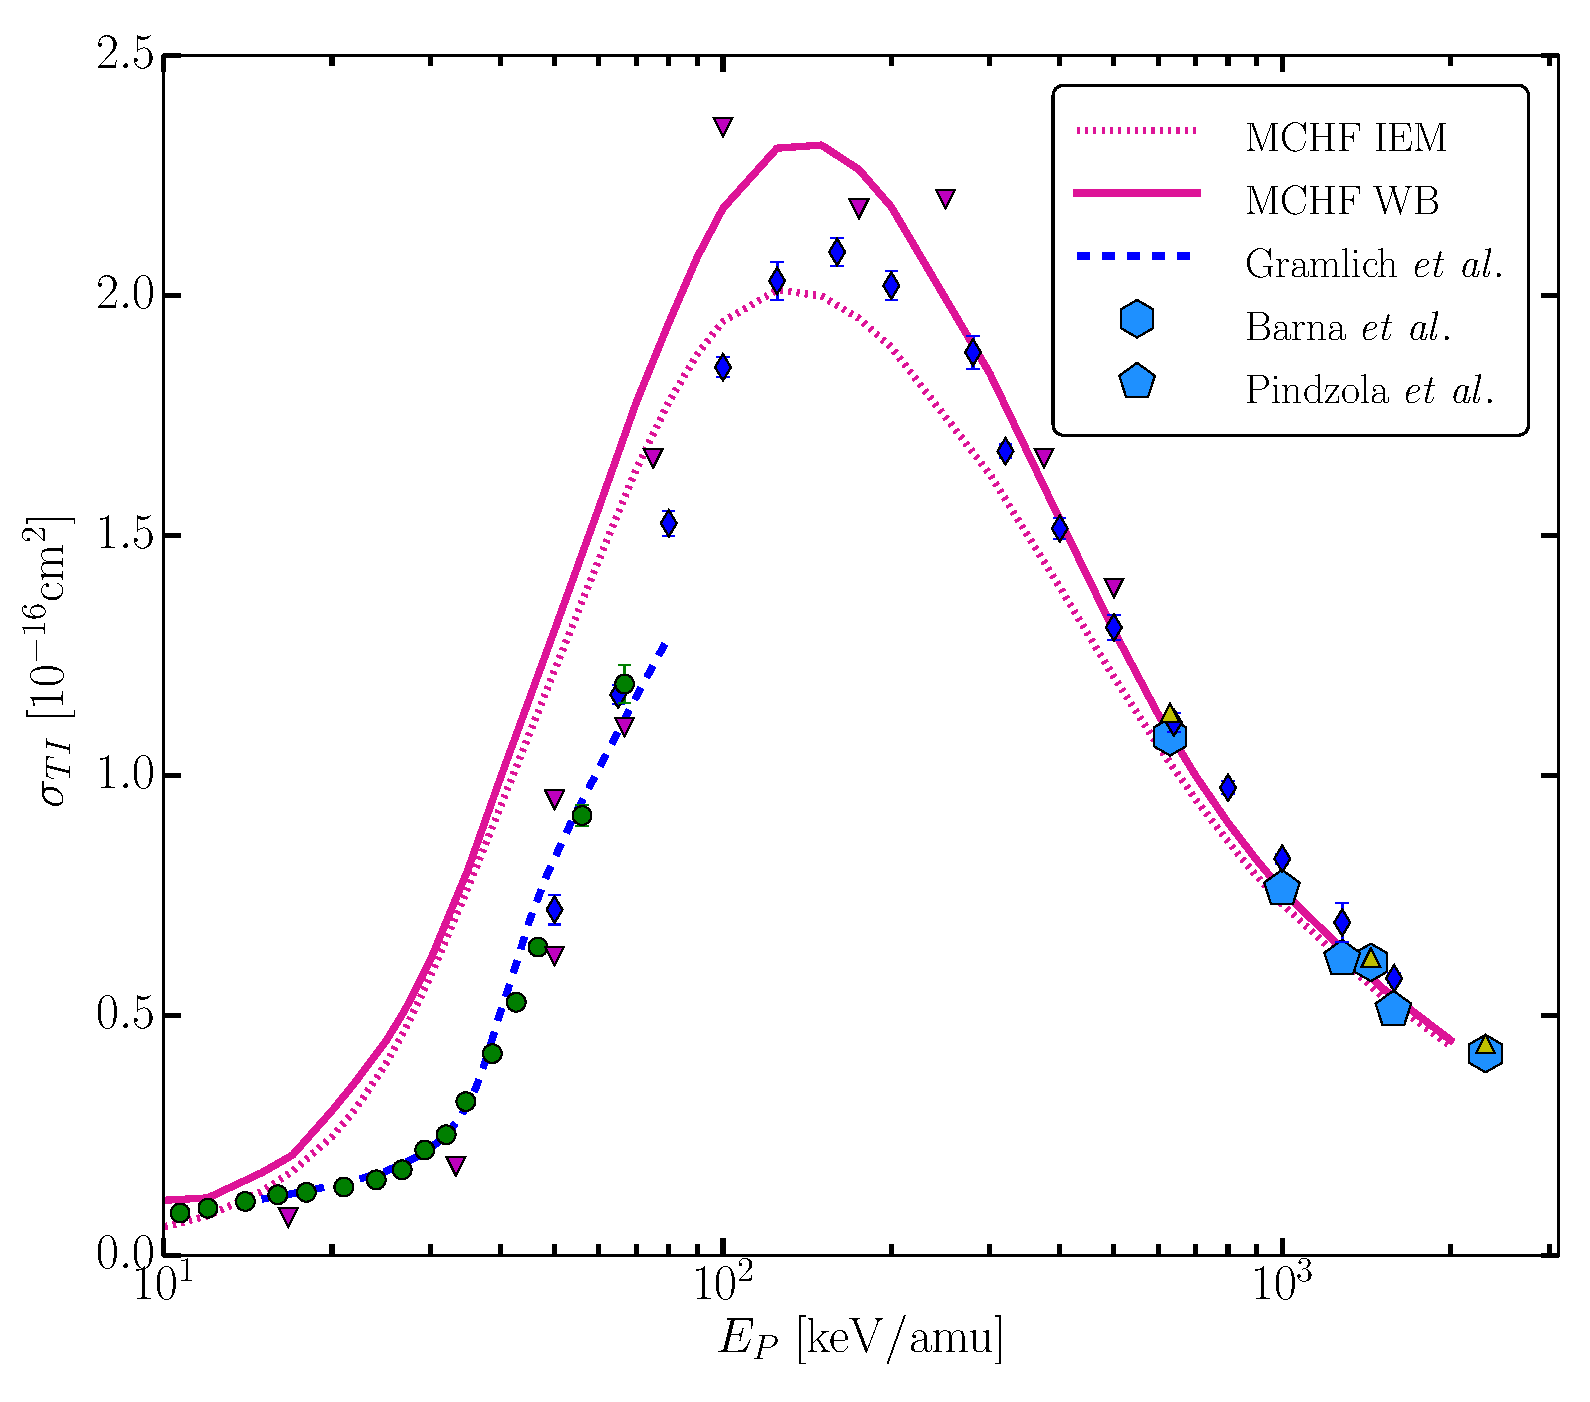
\includegraphics[width = 0.95 \linewidth]{./images/he2phe/he2phe-TI.eps}
            \caption[Total cross section for single ionization of helium by He\textsuperscript{2+}
                     impact.]{Total cross section for single ionization of helium by
                     He\textsuperscript{2+} impact. Theoretical results: Gramlich
                     et al.~\cite{GGS-89}, Barna
                     et al.~\cite{BTB-05}, Pindzola et al.~\cite{PRC-07}.
                     Experimental data: {\color{blue}{$\blacklozenge$}}~\cite{SG85},
                     {\color{OliveGreen}{$\bullet$}}~\cite{SG89},
                     {\color{RedViolet}{$\blacktriangledown$}}~\cite{Dubois87},
                     {\color{GreenYellow}$\blacktriangle$}~\cite{KAH84}. \label{fig:he2phe-ti}}
         \end{figure}

         \begin{figure}[t]
            \centering
            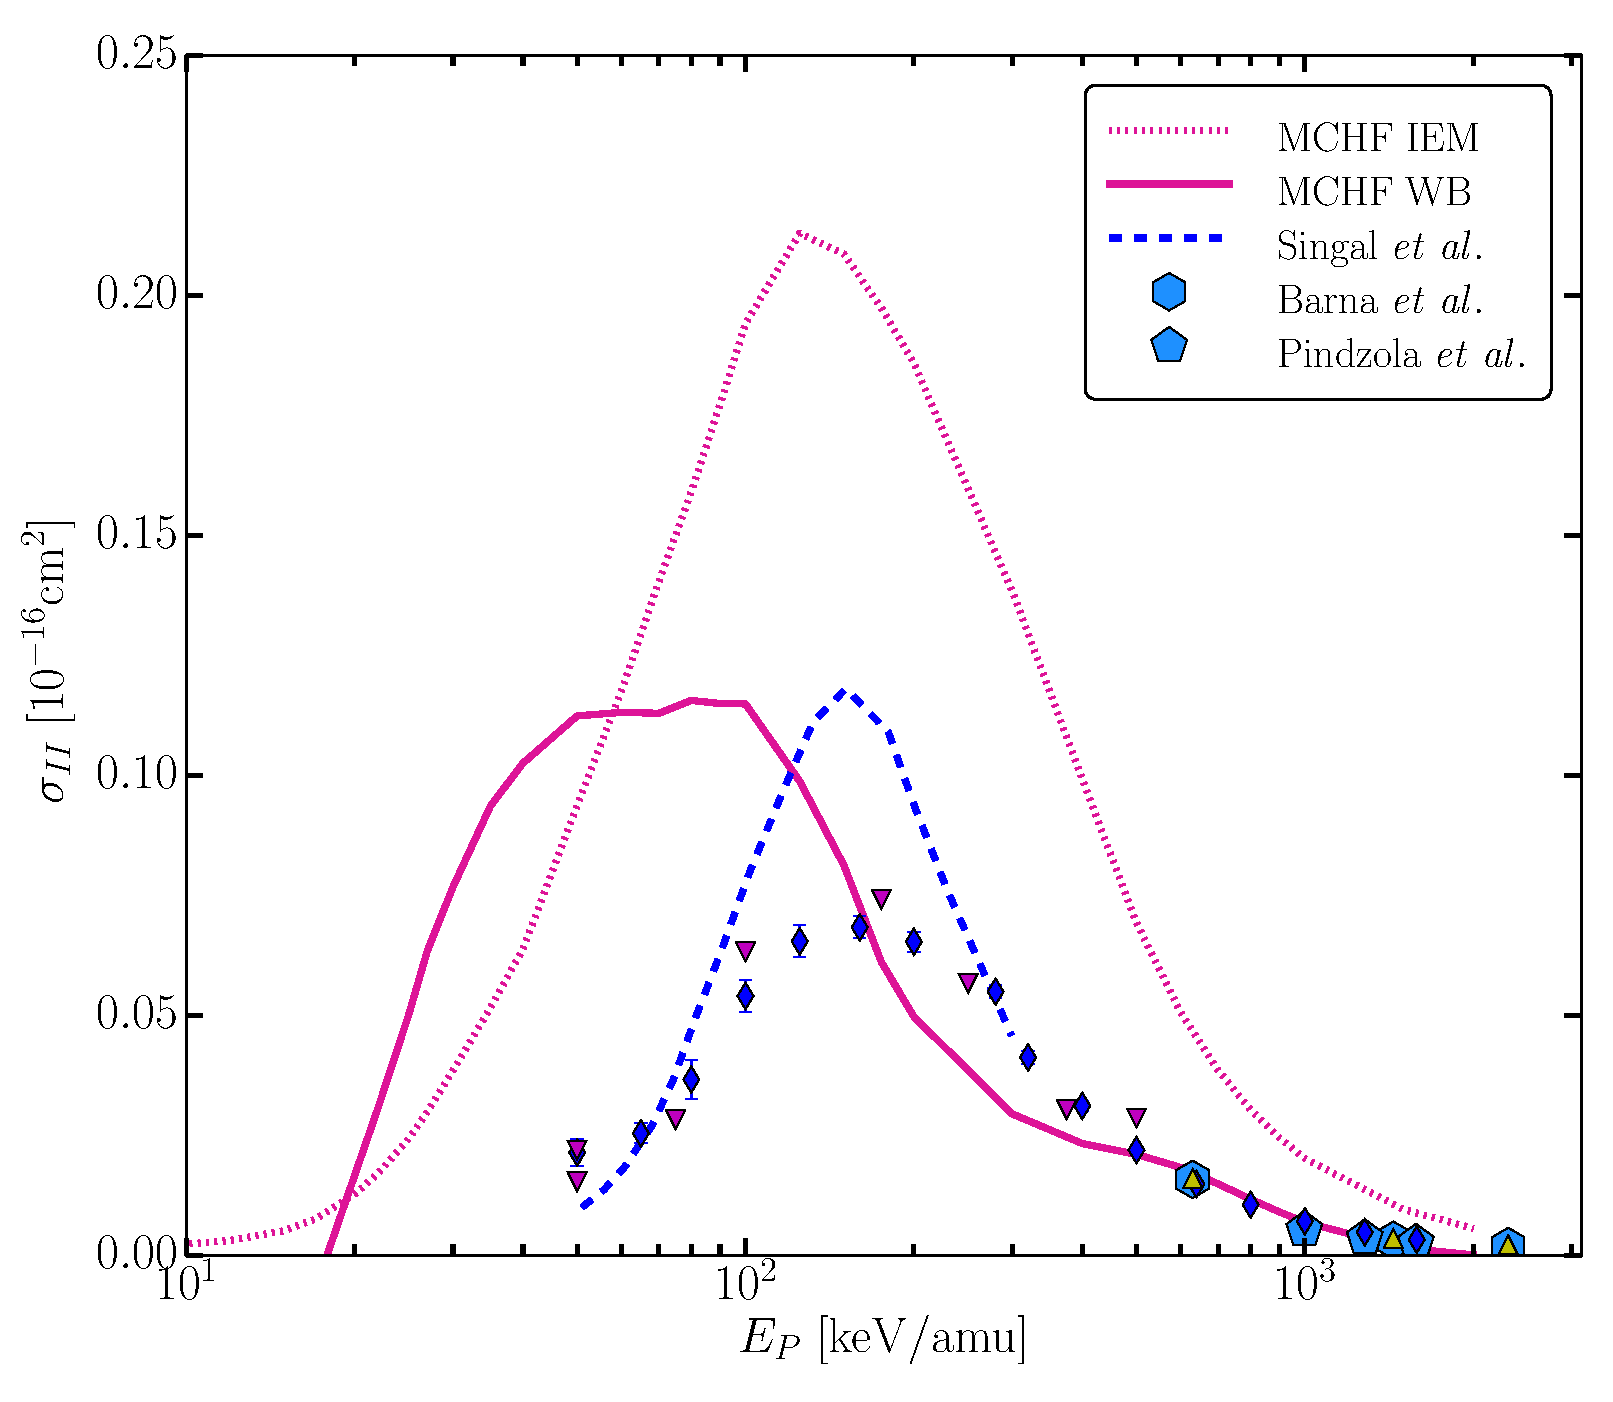
\includegraphics[width = 0.95 \linewidth]{./images/he2phe/he2phe-II.eps}
            \caption[Total cross section for double ionization of helium by He\textsuperscript{2+}
                     impact.]{Total cross section for double ionization of helium by
                     He\textsuperscript{2+} impact. Theoretical results: Singal
                     et al.~\cite{SL-91}, Barna
                     et al.~\cite{BTB-05}, Pindzola et al.~\cite{PRC-07}
                     Experimental data: {\color{blue}{$\blacklozenge$}}~\cite{SG85},
                     {\color{RedViolet}{$\blacktriangledown$}}~\cite{Dubois87},
                     {\color{GreenYellow}$\blacktriangle$}~\cite{KAH84}. \label{fig:he2phe-ii}}
         \end{figure}

         \begin{figure}[ht]
            \centering
            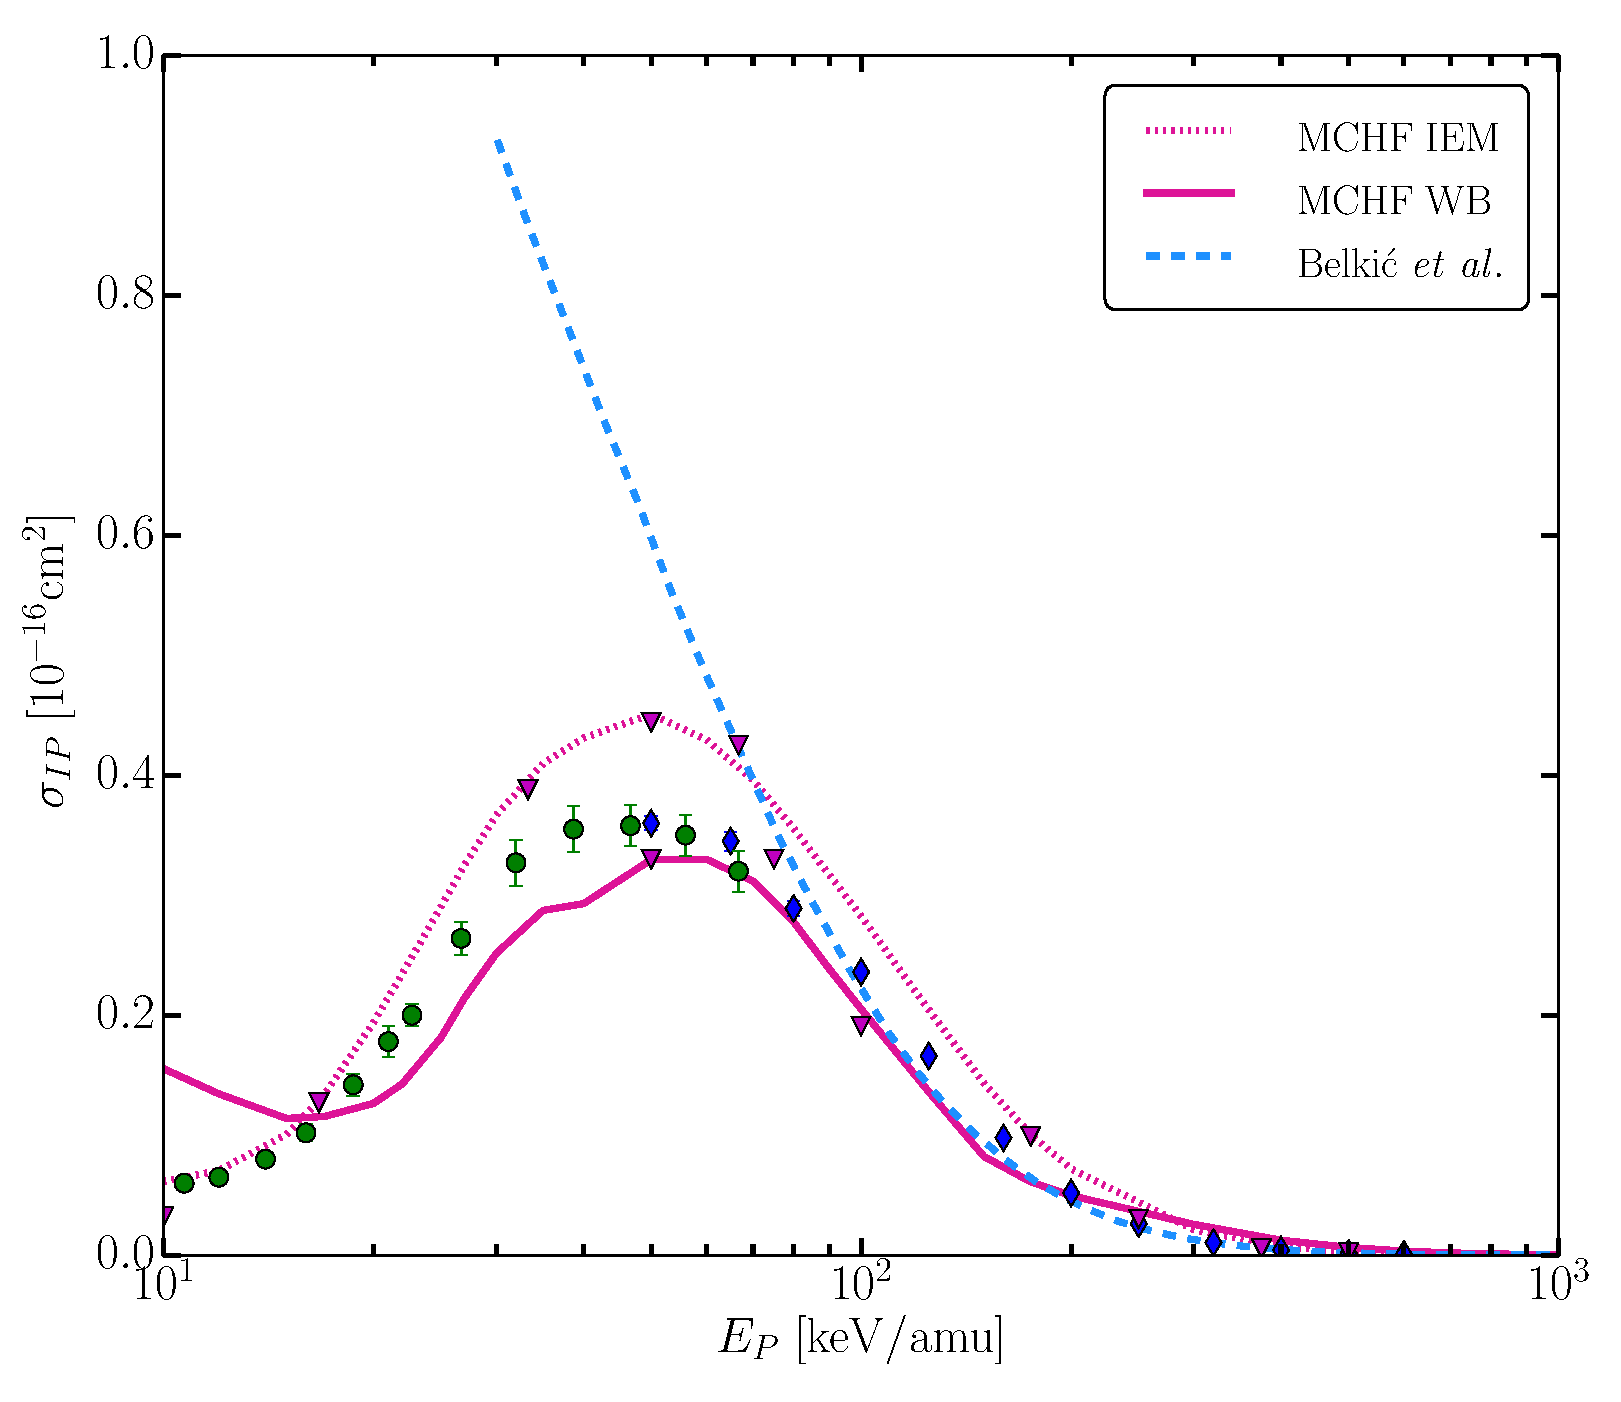
\includegraphics[width = 0.95 \linewidth]{./images/he2phe/he2phe-IP.eps}
            \caption[Total cross section for transfer ionization in He\textsuperscript{2+}-He
                     Collisions.]{Total cross section for transfer ionization in
                     He\textsuperscript{2+}-He Collisions. Theoretical results: Belki\'{c}
                     et al.~\cite{BMM-97}.
                     Experimental data: {\color{blue}{$\blacklozenge$}}~\cite{SG85},
                     {\color{OliveGreen}{$\bullet$}}~\cite{SG89},
                     {\color{RedViolet}{$\blacktriangledown$}}~\cite{Dubois87}. \label{fig:he2phe-ip}}
         \end{figure}

         \begin{figure}[ht]
            \centering
            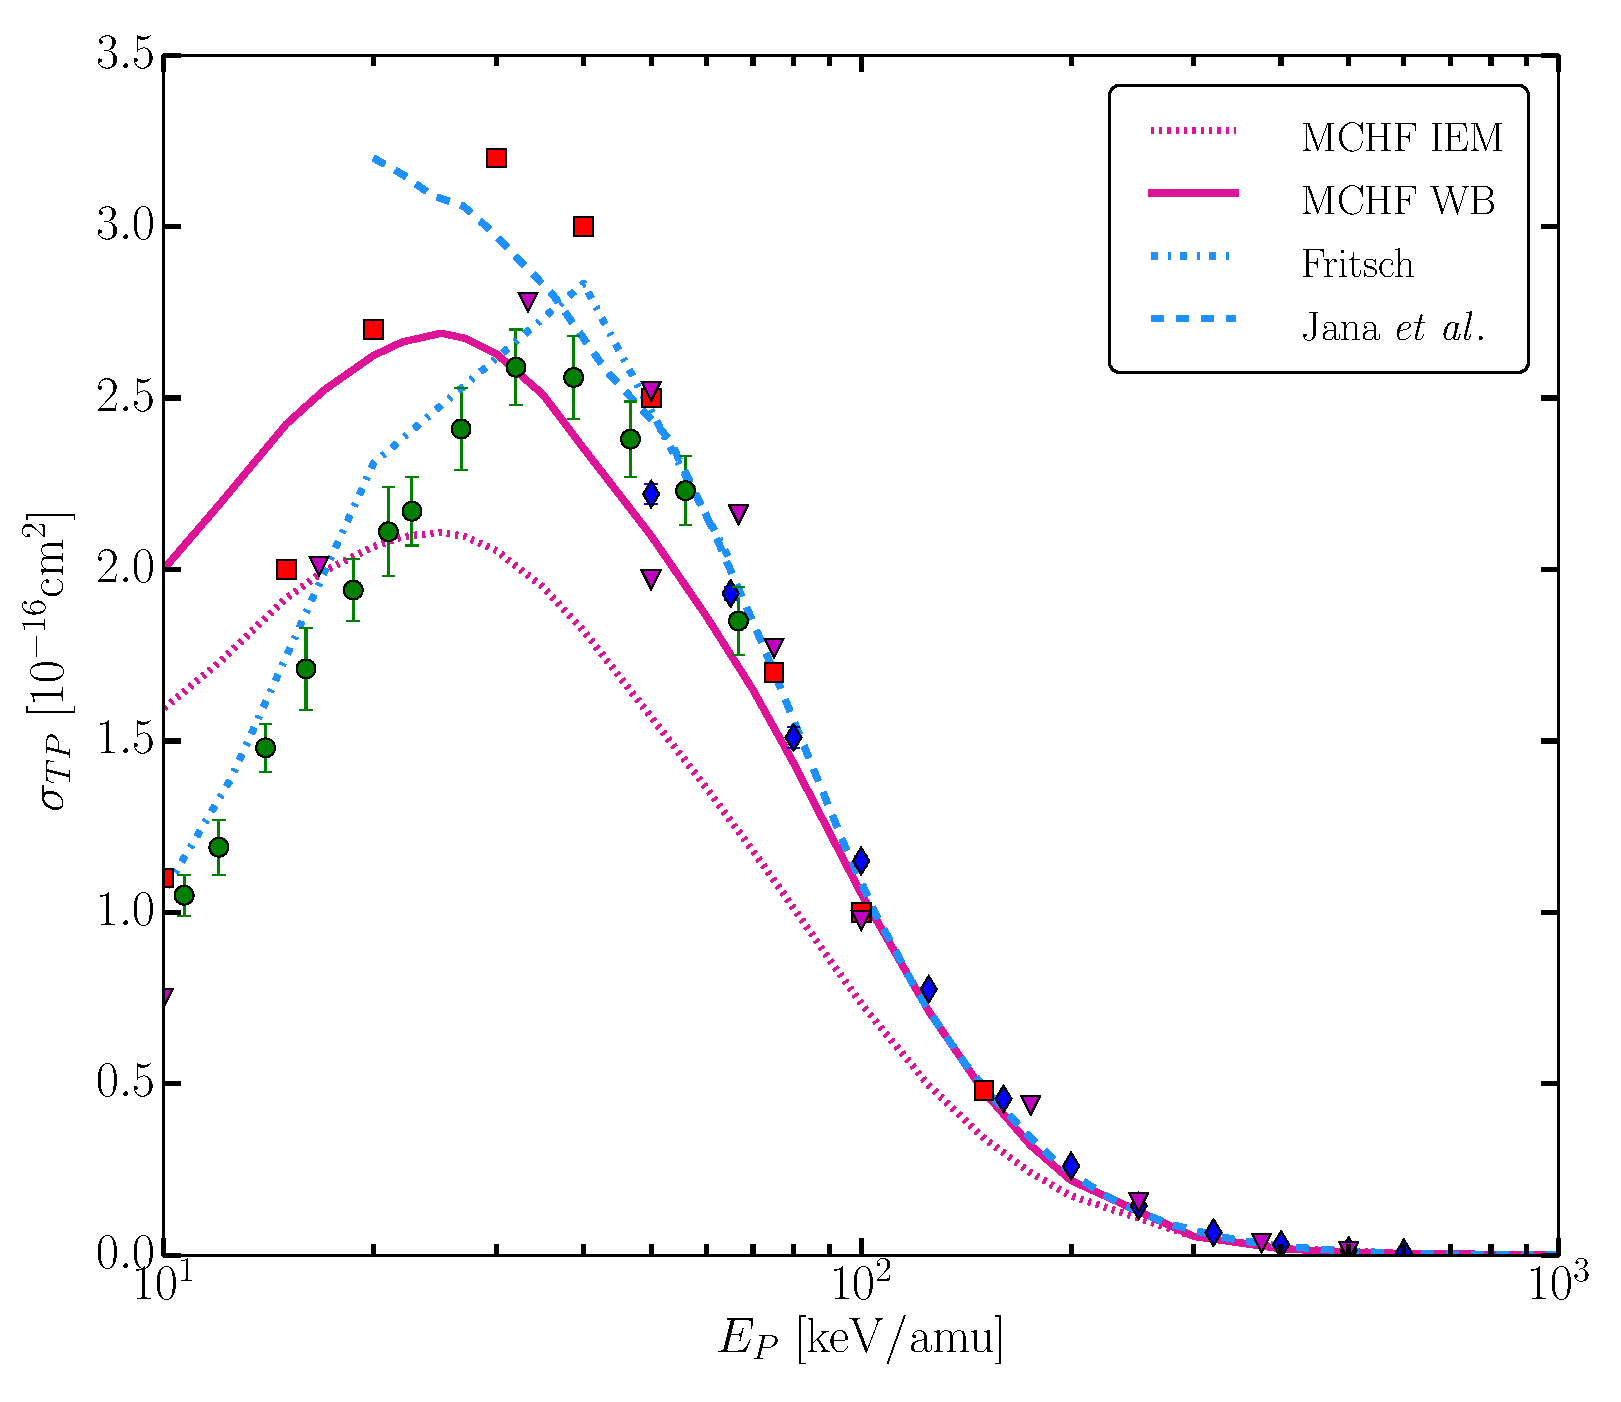
\includegraphics[width = 0.95 \linewidth]{./images/he2phe/he2phe-TP.eps}
            \caption[Total cross section for single capture in He\textsuperscript{2+}-He
                     collisions.]{Total cross section for single capture in He\textsuperscript{2+}-He
                     collisions. Theoretical results: Fritsch~\cite{Fritsch-94} and \textsc{dw-4b} of
                     Jana et al.~\cite{JMP-15}.
                     Experimental data: {\color{blue}{$\blacklozenge$}}~\cite{SG85},
                     {\color{OliveGreen}{$\bullet$}}~\cite{SG89},
                     {\color{RedViolet}{$\blacktriangledown$}}~\cite{Dubois87},
                     {\color{red}$\blacksquare$}~\cite{Rudd85}. \label{fig:he2phe-tp}}
         \end{figure}
 
         \begin{figure}[htp]
            \centering
            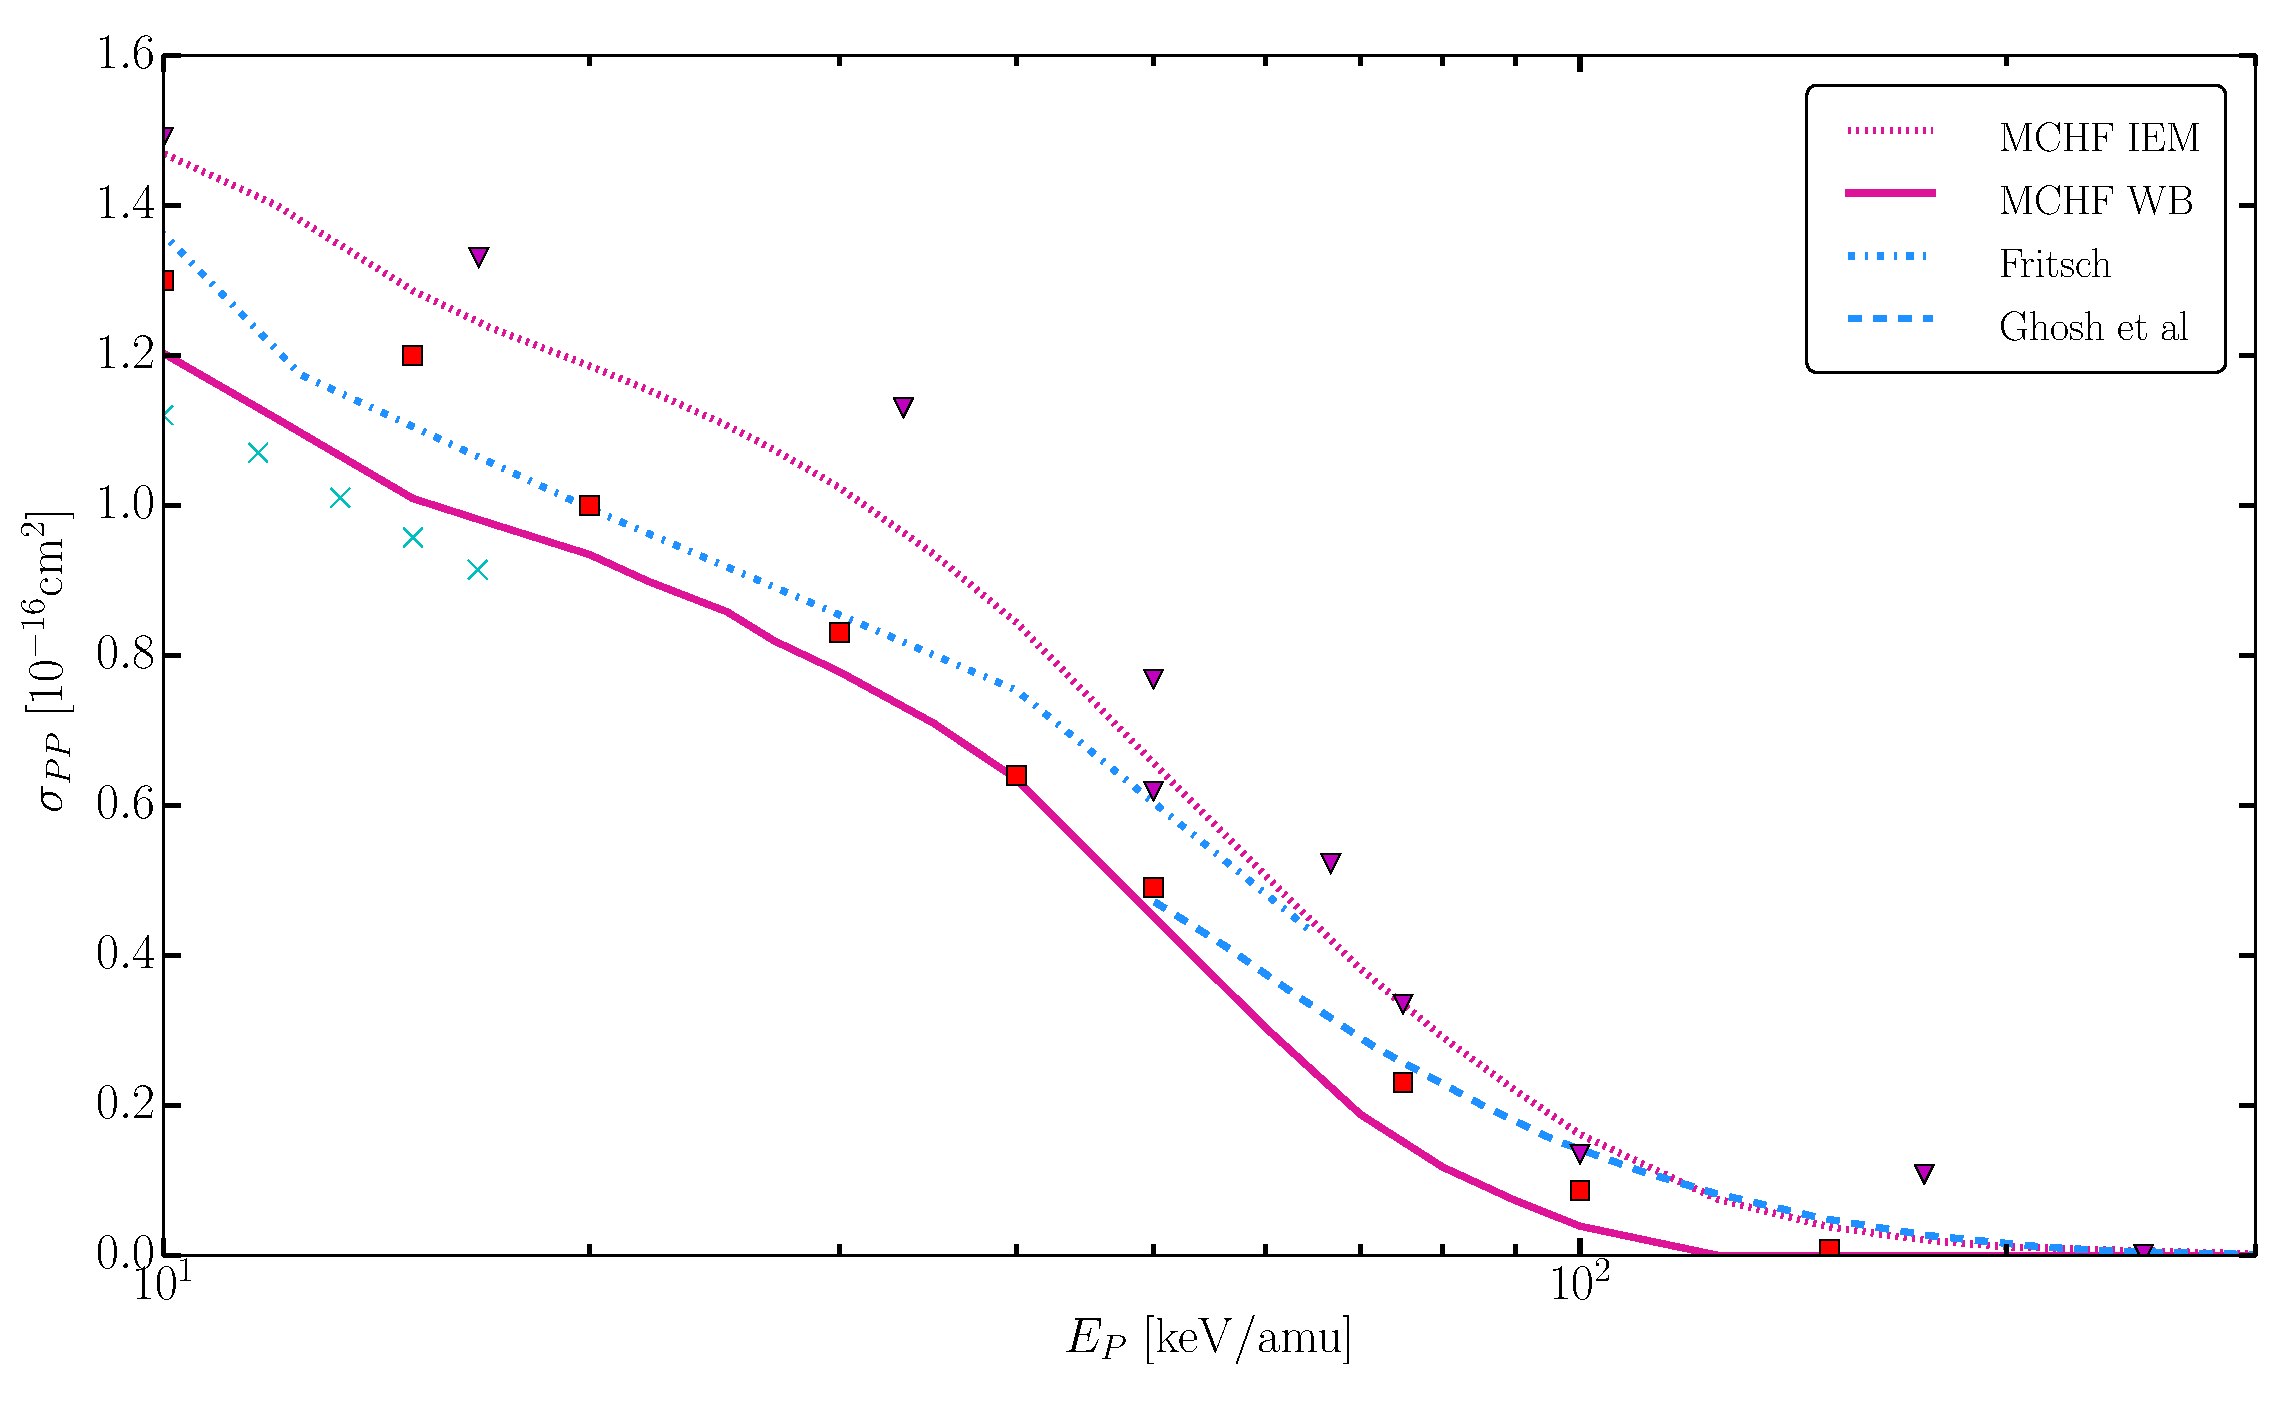
\includegraphics[width = 0.95 \linewidth]{./images/he2phe/he2phe-PP.eps}
            \caption[Total cross section for double capture in He\textsuperscript{2+}-He
                     collisions.]{Total cross section for double capture in He\textsuperscript{2+}-He
                     collisions.
                     Theoretical results: Fritsch~\cite{Fritsch-94} and Ghosh
                     et al.~\cite{GDMP-08}.
                     Experimental data: {\color{RedViolet}{$\blacktriangledown$}}~\cite{Dubois87},
                     {\color{red}$\blacksquare$}~\cite{Rudd85}
                     {\color{TealBlue}$\times$}~\cite{SG74}. \label{fig:he2phe-pp}}
         \end{figure}

         The results of the He\textsuperscript{2+}-He calculations for both \textsc{iem} and \textsc{wb}
         model and experimental data are presented in Figs.~\ref{fig:he2phe-ti}--\ref{fig:he2phe-pp}
         along with an assortment of previous, correlated theoretical calculations. As with our
         proton-helium results single ionization (Fig.~\ref{fig:phe-ti}) in both the \textsc{iem} and
         \textsc{wb} model are quite similar excluding an energy range around the maximum where the
         \textsc{wb} increases the cross section significantly. In both cases the peak appears to be
         shifted to a slightly lower impact energy compared to the measurements. Similar behaviour below
         100~keV/amu see the pair falling above experiment. Depicted along side the current results in
         Fig.~\ref{fig:he2phe-ti} are the previous calculations of Gramlich et al.~\cite{GGS-89}, Barna
         et al.~\cite{BTB-05}, and Pindzola et al.~\cite{PRC-07}. At the high end of the energy range
         explored all results are in agreement. At lower energies (approximately 15--80~keV/amu) the
         results of Gramlich et al.\ are in much better agreement with experiment. This region is
         precisely the range where capture is dominant and quite strong. As a result $p_T < 1/2$ for a
         significant portion of this range causing $I^{TT}_\mathrm{c} = -{p_T}^2$. A negative
         $I^{TT}_\mathrm{c}$ will increase $p^{TI}$, luckily $I^{TP}_\mathrm{c}$ is enough to keep
         \textsc{wb} results from exceeding those of the \textsc{iem}  [cf.\ Eq.~\eqref{eq:pti-ic}]. The
         lack of correlated calculations near the experimental maximum unfortunately means little can be
         concluded in this region of the curve.

         The \textsc{wb} results for double ionization, Fig.~\ref{fig:he2phe-ii}, display the familiar
         pattern seen in both antiproton and proton collisions, namely, fair agreement with experiment
         at high impact energies coupled with overestimation of the data at lower energies and a
         reduction over \textsc{iem}. It should be noted that due to the size of the error bars of the
         low energy $\bar{p}$-He data what constitutes an overestimation is difficult to determine
         (\textsc{wb} results do tend towards the upper limits of these error bars). It would seem that
         such behaviour is a general feature of the \textsc{wb} model. For the positively-charged
         projectiles the \textsc{wb} model causes a shift in the maximum to lower energies. Much like
         the $p$-He results there are slight fluctuations in the He\textsuperscript{2+}-He \textsc{wb}
         results due to instabilities in the dynamics.

         As above Barna et al.\ and Pindzola et al.\ support the high energy \textsc{wb}
         results. Fig.~\ref{fig:he2phe-ii} also includes the results of Singal et al., while
         not a two-electron calculation it incorporates a modified single-particle potential designed to
         account for the increased difficulty of ionizing two electrons. If nothing else these results
         confirm the placement of the position of the \textsc{iem} cross section maximum. This confirms
         the belief that the \textsc{wb} model becomes less dependable at lower energies.

         Unlike for the proton-helium system double ionization and transfer ionization,
         Fig.~\ref{fig:he2phe-ip}, are not identical. The increased role of capture due to the deeper
         potential well of the He\textsuperscript{2+} projectile has the important consequence of
         allowing the $p_P$ to rise above the critical one half threshold. As a result
         $I^{PP}_\mathrm{c}$ is no longer trivial, and the bounds defining $I^{TP}_\mathrm{c}$ vary more
         freely. The \textsc{wb} model reduces \textsc{iem} results through most of the impact energy
         range. A slight over-reduction occurs to the left of the peak. Below 20~keV/amu the results
         begin to swing drastically upwards to compensate for the fact that double ionization becomes
         zero in this region. As mentioned above the ripples present in the \textsc{wb} curve are due to
         instabilities in the dynamics.

         Much like the $p$-He system few calculations exist beyond the level of the \textsc{iem} for the
         transfer ionization channel. Presented is the post form of the four-body continuum
         distorted-wave  approximation results of Belki\'{c} et al.~\cite{BMM-97}. As mentioned above
         the post form includes explicit dynamic correlation. At the extremes of the energy range
         Belki\'{c} et al. are in better agreement with experiment, as the \textsc{wb} and \textsc{iem}
         slightly exaggerate the cross section (similar to the $p$-He results). These discrepancies
         become larger as the peak is approached from above. It is difficult to ascertain how much of
         this widening gap between our \textsc{wb} results and Belki\'{c} et al.'s calculation is a
         result of the increased importance of dynamic correlation. Certainly this is the primary
         difference down to 80~keV/amu, below which point the perturbative calculation appears to break
         down making it of less utility for the current purpose.
 
         Single capture cross sections, presented in Fig.~\ref{fig:he2phe-tp}, also follow a pattern
         similar to that laid out by the proton-helium case: an increase in the \textsc{wb} over
         \textsc{iem}. This increase results in good agreement with experiment above 50~keV/amu. Unlike
         previous results the enhancement in cross section persists to low energies, where the
         \textsc{wb} model overestimates the  measurements.

         In the high energy region of the curve the \textsc{wb} model is in fair agreement with the
         \textsc{dw-4b} results of Jana et al. It would appear the effects of dynamic correlation may
         account for the slight underestimation of the \textsc{wb} model to the right of the maximum.
         Below the peak the coupled channel results of Fritsch~\cite{Fritsch-94} lend credence to the
         experimental data. The failure of both the \textsc{wb} and \textsc{iem} models to agree with
         these results (and by extension experiment) may point to a possible failure of the underlying
         dynamic calculation in separating the target, projectile and ionizing regions ($T$, $P$ and
         $I$).

         As mentioned above the expanded role of capture causes the correlation integral
         $I^{PP}_\mathrm{c}$ to no longer be trivial. This also means that double capture in the
         \textsc{wb} model is no longer identically zero. Results for double capture are presented in
         Fig.~\ref{fig:he2phe-pp}. While the \textsc{wb} decreases the cross section below \textsc{iem}
         it is difficult to conclude whether this is an improvement due to the relatively wide spread in
         the experimental data.

         To aid in this determination we compare our results to those of Fritsch~\cite{Fritsch-94} and
         the post form of the four-body boundary corrected continuum intermediate state approximation
         (\textsc{bccis-4b}) results of Ghosh et al.~\cite{GDMP-08}. For the highest energies presented
         Ghosh et al.\ support the results of the \textsc{iem} over those of the \textsc{wb} model. In
         this region the same factors that force the $p$-He \textsc{wb} double capture channel to be
         identically zero force cross sections above 125~keV/amu into triviality. Below this limit Ghosh
         et al.\ begin to fall more in line with the \textsc{wb} results. As the results of Fritsch
         enter the picture in the lower portion of the energy range the \textsc{wb} model appears to be
         favoured, the gap between Fritsch and the \textsc{wb} being less than that between \textsc{iem}
         and Fritsch. The remaining discrepancy may be due once again to dynamic correlation effects.

      \end{subsection}

   \end{section}

\end{chapter}

\begin{chapter}{\texorpdfstring{He\textsuperscript{+}}{He+}-He Collisions \label{chap:hephe}}

   The investigations of the previous chapter began with the simplest possible multi-electron collision
   system, one where a positively-charged projectile is incident on a helium like target. The situation
   was then complicated by allowing the projectile to be negative, thus forcing one to consider electron
   transfer in addition to ionization processes.

   In this chapter the system of interest is expanded further by the inclusion of an active electron on
   the projectile. More specifically, the remainder of this work concerns itself primarily with the
   He-He\textsuperscript{+} collision system.

   While the external potential, $v_\mathrm{ext}$, maintains the form of Eq.~\eqref{eq:phe2p-ext} and the
   spin-polarized nature of the collision system means that the spin-free description utilized in the
   previous chapter is no longer applicable, the full spin-dependent \textsc{tdks} presented in
   Eq.~\eqref{eq:tdks} must be solved.

   The determination of a spin-dependent exchange-correlation potential forms the bulk of this chapter
   (Sec.~\ref{sec:pot}) in which a procedure for calculating an accurate exchange potential within the
   x-only approximation is discussed. This is followed by a brief discussion of the method used to
   extract cross sections from the one-particle density (Sec.~\ref{sec:hephe-det}) before presenting
   results in Sec.~\ref{sec:hephe-res}.

   \begin{section}{Calculating the x-Potential \label{sec:pot}}

      An accurate exchange-potential is essential for a precise description of the
      He\textsuperscript{+}-He collision system. The spin polarized nature of the system, which
      emphasizes exchange effects (i.e manifestations of Fermi statistics), make this fact indisputable.

      As discussed in Sec.~\ref{sec:opm}, within the x-only approximation, the exchange-potential may be
      determine exactly via the \textsc{opm}. As this process is prohibitively expensive the \textsc{kli}
      approximation which, as has been mentioned in Sec.~\ref{sec:kli}, produces similar results was
      used in its stead.

      At any instant of time, $t$, the He\textsuperscript{+}-He system may be regarded as a diatomic
      molecule with an internuclear distance $R_\mathrm{int}(t) = \sqrt{b^2 + z(t)^2}$, where $b$ and
      $z$ are the impact parameter and $z$ position of the projectile (as described in
      Chap.~\ref{chap:p-he2p-he}). The \textsc{dft} molecular structure package \texttt{DIAMOL} has been
      designed precisely for such situations ({\color{red}{not sure how to cite this}}). If at each
      time-step of the \texttt{BGM} (the software package which implements the \textsc{bgm}) the
      time-dependent \textsc{ks}-orbitals, $\varphi_{\sigma j}(\mathbf{r},t)$ is fed into
      \texttt{DIAMOL} the exchange-potential, $v^{\sigma}_\mathrm{x}[\varphi_{\sigma j};t]$, may be
      calculated at each $t$, effectively giving one the
      time-dependent exchange-potential $v^{\sigma}_\mathrm{x}[\varphi_{\sigma j}](t)$.

      Limitations of \texttt{DIMAOL} complicate this procedure. Whereas $\varphi_{\sigma j}$ have no
      enforced symmetry, \texttt{DIAMOL} assumes that the orbitals are cylindrically symmetric about the
      internuclear axis. To avoid conflicts only a cylindrically symmetric portion of the
      \textsc{ks}-orbitals can be fed into \texttt{DIAMOL}. In order to describe a work around to this
      problem one must first understand how the \textsc{ks}-orbitals are represented within the
      \textsc{bgm}.

      Each \textsc{ks}-orbital is represented as a sum
      %
      \begin{equation} \label{eq:bgmexp}
         \varphi_{\sigma j}(\mathbf{r},t) = \sum d_{c k L M}^{\sigma j} \tilde{\chi}^{LM}_{c k},
      \end{equation}
      %
      where $c$ labels the centres, target ($T$) and projectile ($P$), and the remaining indices are
      identical to the ones described in Eq.~\eqref{eq:bgmbasis}. The functions
      $\tilde{\chi}^{00}_{c k}$ are given by
      %
      \begin{equation} \label{eq:etfbasis}
         \tilde{\chi}^{00}_{ck} =
            \begin{cases}
               e^{i \mathbf{v}_T \cdot \mathbf{r}} {\chi}^{00}_{c k} & c = T, \\
               e^{i \mathbf{v}_P \cdot \mathbf{r}} {\chi}^{00}_{c k} & c = p,
            \end{cases}
      \end{equation}
      %
      where $\chi^{00}_{c k}$ are, once again, the eigenstates of the undisturbed centres, helium
      \textsc{opm} ground-state orbitals on the target and hydrogen-like states on the projectile. The
      difference is the inclusion of the  electron translation factors (\textsc{etf}).

      Leaving aside the \textsc{etf}'s for the time being, it is immediately clear that the simplest way
      to maintain cylindrical symmetry is to only pass the $1s$ contributions on each centre to
      \texttt{DIAMOL}. We must then define the new orbitals
      %
      \begin{equation} \label{eq:1sonly}
         \tilde{\varphi}_{\sigma j} = \tilde{d}^{\sigma j}_T \tilde{\chi}^{00}_{T1} +
                                      \tilde{d}^{\sigma j}_P \tilde{\chi}^{00}_{P1},
      \end{equation}
      %
      where the coefficients $\tilde{d}^{\sigma j}_c$ are defined in terms of the projection operator,
      %
      \begin{equation} \label{eq:proj}
         \hat{P} = \sum\limits_{c_1, c_2 \in \{T,P\}} \tilde{S}^{-1}_{c_1 c_2}
                                                      \ket{\tilde{\chi}^{00}_{c_1 1}}
                                                      \bra{\tilde{\chi}^{00}_{c_2 1}}
      \end{equation}
      %
      with $\tilde{S}^{-1}_{c_1 c_2}$ the inverse of the overlap matrix
      %
      \begin{equation}
         \tilde{S}_{c_1 c_2} = \braket{\tilde{\chi}^{00}_{c_1 1} | \tilde{\chi}^{00}_{c_2 1}},
      \end{equation}
      %
      by
      %
      \begin{equation} \label{eq:ceofproj}
         \tilde{d}^{\sigma j}_c = \braket{\tilde{\chi}^{00}_{c 1} | \hat{P} |\tilde{\varphi}_{\sigma j}}.
      \end{equation}

      It can be easily shown that the \textsc{etf}'s introduce addition asymmetries. Working in the
      rotating centre of mass frame, the coordinate system used by \texttt{DIAMOL}, the \textsc{etf}'s
      become
      %
      \begin{subequations} \label{eq:etf}
         \begin{equation} \label{eq:etfT}
            e^{i \mathbf{v}_T \cdot \mathbf{r}} =
             e^{\frac{i v_\mathrm{rel}}{2} (x \sin \theta - z \cos \theta)},
         \end{equation}
         %
         \begin{equation} \label{eq:etfP}
            e^{i \mathbf{v}_P \cdot \mathbf{r}} =
             e^{\frac{i v_\mathrm{rel}}{2} (z \cos \theta - x \sin \theta)},
         \end{equation}
      \end{subequations}
      %
      where $v_\mathrm{rel}$ is the relative velocity of the centres and $\theta = \arctan b/z$. The
      explicit $\phi$ dependence introduced by the $x$-components of the \textsc{etf}'s break
      cylindrical symmetry (refer to Sec.~\ref{sec:prolate}). To preserve cylindrical symmetry there are
      two options.
      
      The obvious first option is to ignore the \textsc{etf}'s or, equivalently, set them to 1. The
      second option is to include only the $z$-components. It should be noted that as $z$ approaches 0
      the two options become equivalent, thus any benefit derived from a partial \textsc{etf} will be
      lost near the closet approach.

      Any investigation of the impact of the \textsc{etf}'s is best carried out in an isolated
      environment. To achieve this we may introduce a no-response model. In such a model the initial
      occupations of the orbitals passed to \texttt{DIAMOL} will be frozen and the full orbitals will
      be propagated in the resulting potential. To be more concrete, if we have two spin-up and one
      spin-down electron the coefficients be given the fixed values
      %
      \begin{equation} \label{eq:noresp}
         \tilde{d}^{\uparrow 1}_T = \tilde{d}^{\uparrow 2}_P = \tilde{d}^{\downarrow 1}_T  = 1
         ~~~ \mbox{and} ~~~
         \tilde{d}^{\uparrow 1}_P = \tilde{d}^{\uparrow 2}_T = \tilde{d}^{\downarrow 1}_P  = 0.
      \end{equation}
      %
      In this way the only phase information entering \texttt{DIAMOL} will arise directly from the
      \textsc{etf}'s.

      Regardless of which orbitals are passed to \texttt{DIAMOL} it is important that the same orbitals
      used to calculate $v_\mathrm{x}$ are used in the determination of $v_\mathrm{H}$. As one of the
      primary functions of the exchange-potential is the  cancellation of the self-interaction present
      in the Hartree potential they must both be constructed consistently with each other lest the
      self-interaction remain. For this reason, and for ease of future discussion, we will define a
      combine electron-electron potential
      %
      \begin{equation} \label{eq:vee}
         v_\mathrm{ee} = v_\mathrm{x} + v_\mathrm{H}.
      \end{equation}

   \end{section}

   \begin{section}{Results I Guess? \label{sec:hephe-res}}

      \begin{subsection}{1\textit{s}-only Toy Model \label{sec:toy}}

         \begin{figure}[htp]
            \centering
            \begin{subfigure}{.5\textwidth}
               \centering
               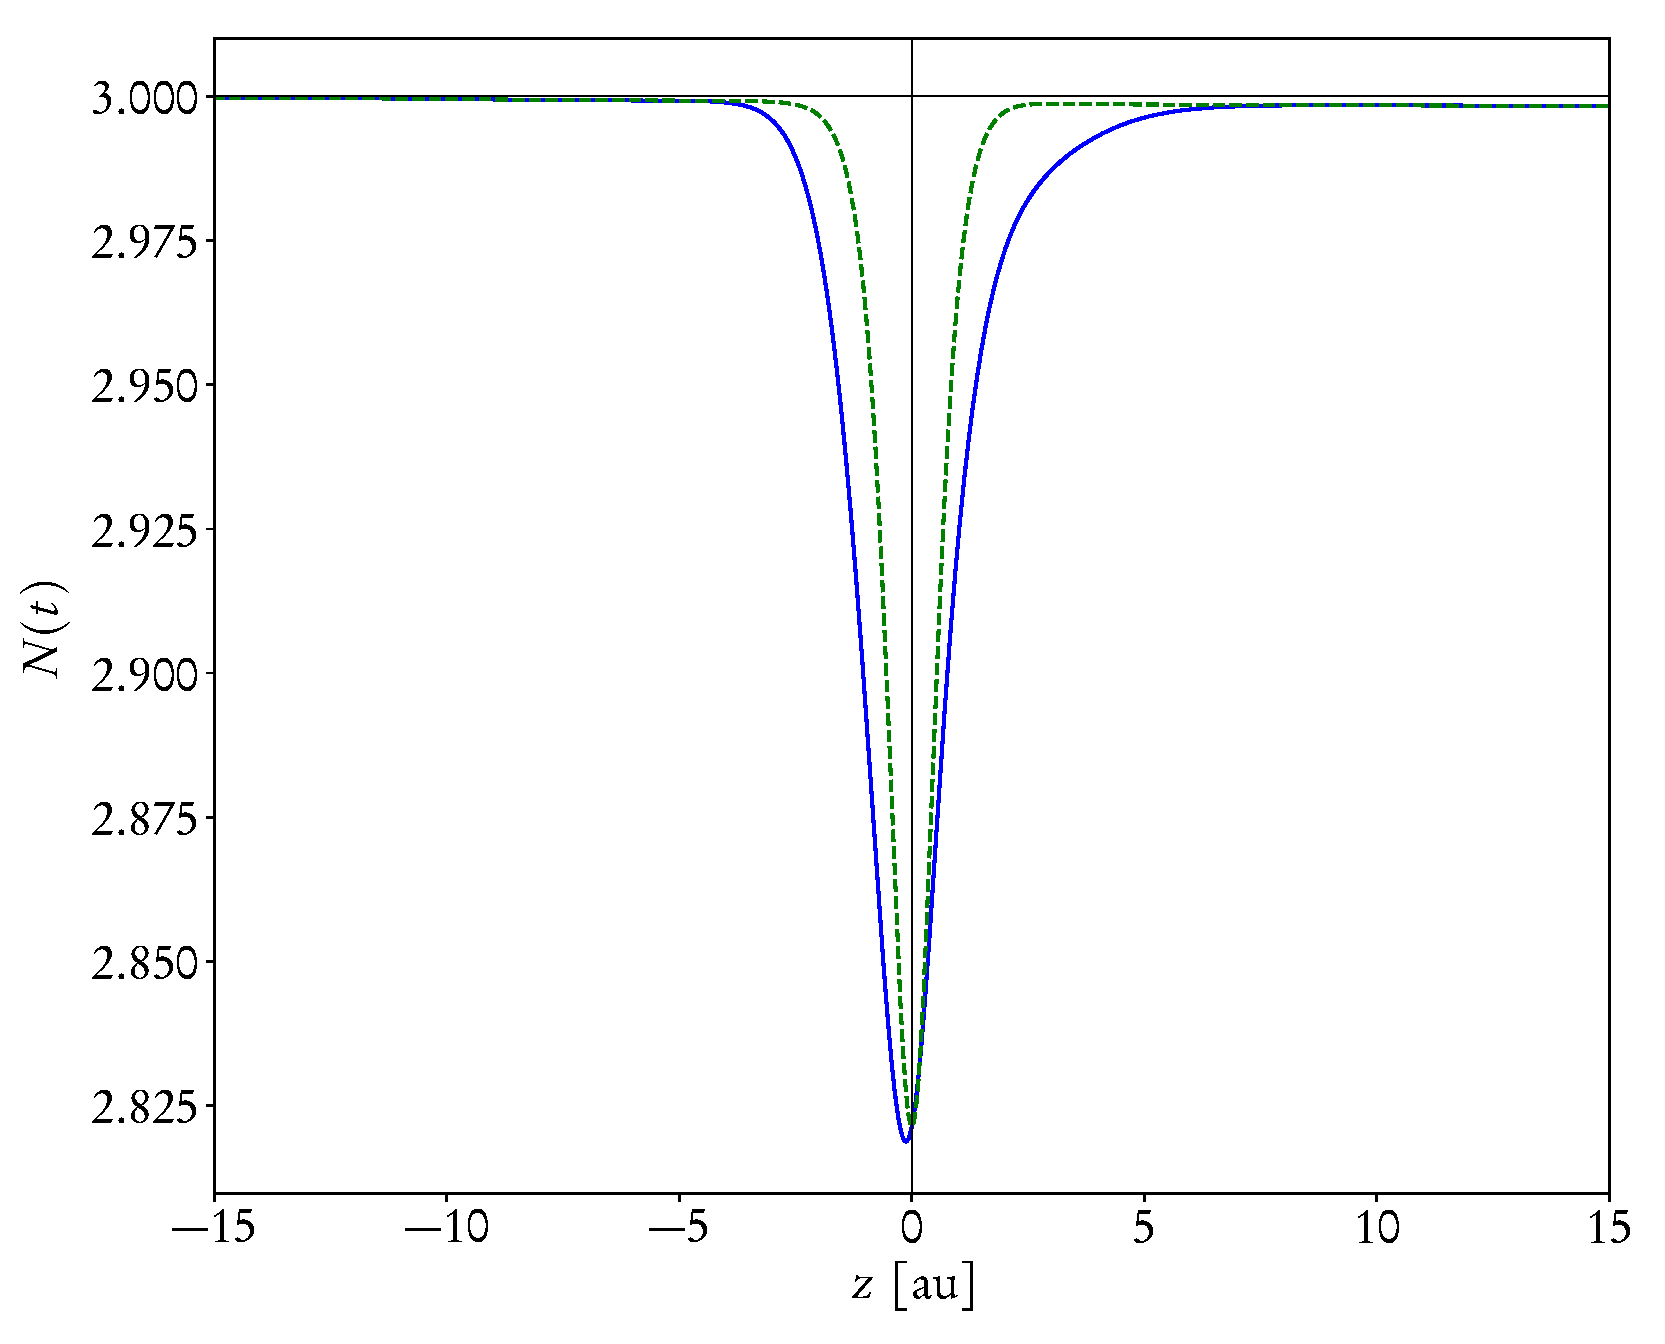
\includegraphics[width=\linewidth]{./images/toymodel/dNorm-1s-20.eps}
               \caption{$E_P = 20 \mathrm{keV}/\mathrm{amu}$. \label{fig:toy20}}
            \end{subfigure}%
            \begin{subfigure}{.5\textwidth}
               \centering
               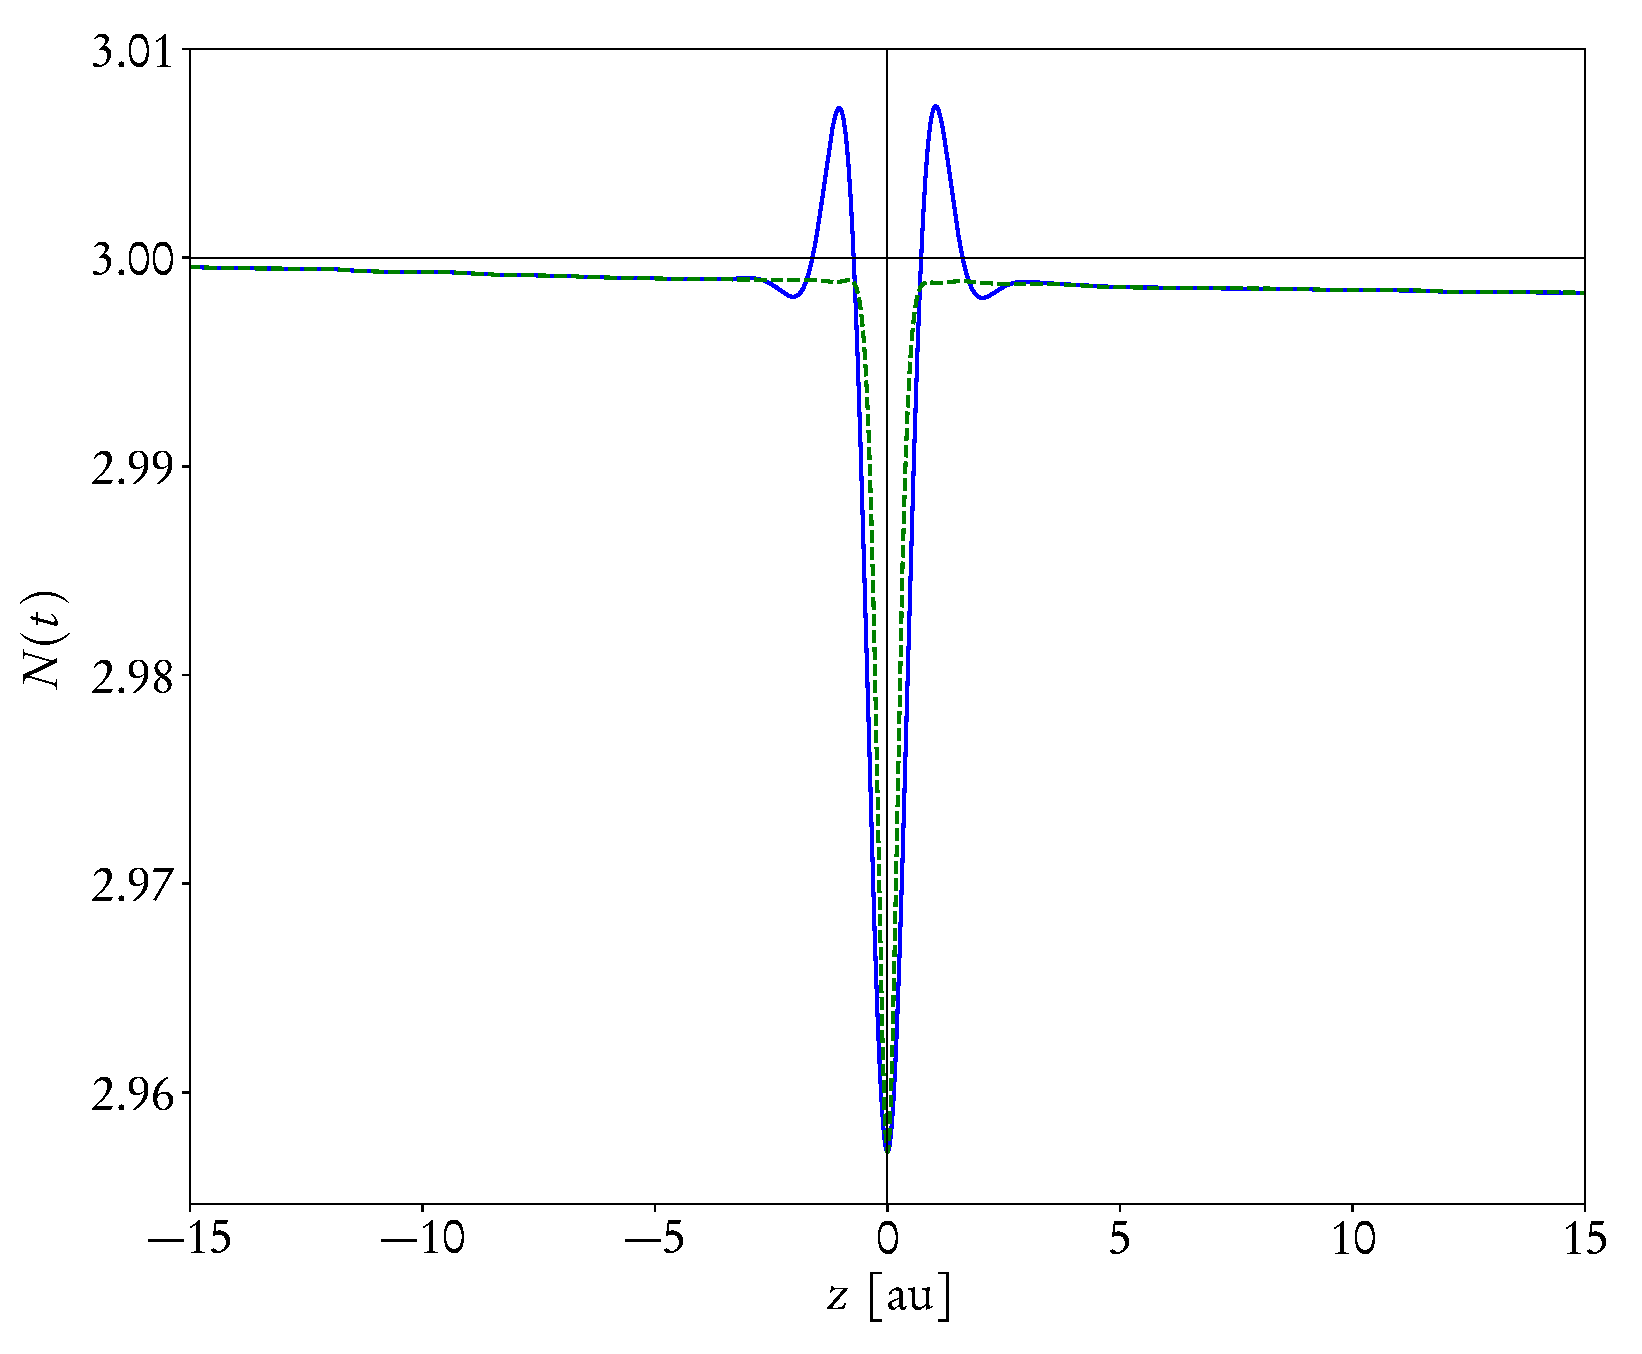
\includegraphics[width=\linewidth]{./images/toymodel/dNorm-1s-1000.eps}
               \caption{$E_P = 1000 \mathrm{keV}/\mathrm{amu}$. \label{fig:toy1000}}
            \end{subfigure}
            \caption[Number of particles as a function of \textit{z} in 1\textit{s}-only toy model]
                    {Number of particles as a function of $z$ in 1$s$-only toy model for $b = 1.0
                    \mathrm{au}$. In both panels; solid line: \textsc{etf} off, dashed line:
                    \textsc{etf} on. \label{fig:toy}}
         \end{figure}

         Before presenting the results for the full system some of the details of a simplified toy model
         will be discussed. In this model only the $1s$ target and projectile states are included in
         the \textsc{bgm} basis. In this way one can ensure that the orbitals propagated by the dynmaics
         code are the same as those passed into \texttt{DIAMOL}.

         A useful quantity to monitor is the norm of the one-particle density,
         %
         \begin{equation}
            N(t) = \int \mathrm{d}^3 r \, n(\mathbf{r},t).
         \end{equation}
         %
         Ionization having been excluded by construction within this model one should find $N(t) = 3$
         for all time, major violations of this can only be associated with the \textsc{etf}'s.

         Figures~\ref{fig:toy20} and \ref{fig:toy1000} display $N$ as a function of $z$ for collisions
         with impact energy of 20 keV/amu and 1000 keV/amu respectively. Both calcualtions use an impact
         parameter of 1 au. While both the curves representing calculations including and excluding the
         partial \textsc{etf}'s show sizable norm violations the inclusion of a partial \textsc{etf}
         offers clear benefits. The \textsc{etf}'s reduce the overall size of the vioaltions and reduce
         the range of time overwhich these violations occur, this can bee seen most clearly in
         Fig.~\ref{fig:toy20} where the dashed curve detaches from the $N = 3$ line more slowwly and
         reattaches more quickly. Additionally including \textsc{etf}'s corrects the unexpected asymetry
         about $z = 0$.

         The slight loss of norm noticable in the tails of all four curves is on the order of $0.002$.
         One can consider the small violation as a limit on the accuracy of calculations. This error is
         on the order of $0.06 \%$.

         The origins of the norm violations is easy to trace. According to Eq.~\eqref{eq:dendef2} the
         one-particle density may be written
         %
         \begin{equation} \label{eq:toyden}
            n(\mathbf{r},t) = \left| \varphi_{\uparrow 1}\right|^2
                            + \left| \varphi_{\uparrow 2}\right|^2
                            + \left| \varphi_{\downarrow 1}\right|^2.
         \end{equation}
         %
         Each orbital in the above expression is normalized to 1 and takes the form
         %
         \begin{equation}
            \varphi = d_T e^{i \mathbf{v}_T \cdot \mathbf{r}} \chi_T
                    + d_C e^{-i \mathbf{v}_T \cdot \mathbf{r}} \chi_C.
         \end{equation}
         %
         Every orbital then contributes
         %
         \begin{equation}
            \int \mathrm{d}^3 r \, \left| \varphi \right|^2 = \left| d_T \right|^2 
                                                            + \left| d_P \right|^2
            + \Re \left[ {d_T}^* d_P \tilde{S}_{TP} \right]
         \end{equation}
         %
         to $N$, where $\tilde{S}_{TP}$ are the matrix elements of the overlap matrix (including
         \textsc{etf}'s). It can then be seen that norm violations are due to the fact that
         \texttt{DIAMOL} cannot fully account for the overlaps of the \textsc{ks}-orbitals, a direct
         consequence of its inability to deal with non-cylindrically symmetric orbitals.

      \end{subsection}

   \end{section}

   \begin{itemize}

      \item Determinental analysis~\cite{inc-prob}.

      \item Spline error bounds~\cite{spline-err}, numerical derivatives~\cite{numdiff1, numdiff2}
      
      \item detailed balance~\cite[p.\ 143--152]{scattering}

      \item Experimental data:~\cite{DT-88, Dub-89, FTFHLP-95, SSMSM-11}

      \item Other calculations: Monte Carlo~\cite{CC-07}, Bohr–Lindhard~\cite{DYC-08, DLZ-12},
         independent event model~\cite{SM-03}, perturbation theory~\cite{Mancev-07, MG-10, GG-12b}.

      \item $\acute{\imath}$ \'{\i} \'{i}

   \end{itemize}

\end{chapter}

\begin{chapter}{Conclusion \label{chap:con}}

   \begin{section}{\texorpdfstring{$p$}{p}-He and \texorpdfstring{He\textsuperscript{2+}}{He2+}-He
                   Collisions \label{sec:con-phe2p-he}}

      We have investigated correlation effects in $p$-He and He\textsuperscript{2+}-He collisions. By
      expanding the correlation integral model of Wilken and Bauer~\cite{wb} applied previously to the
      antiproton-helium system~\cite{pbarhe} we have produced total cross sections for single, double,
      and transfer ionization as well as single and double capture. In order to incorporate electron
      capture processes into the \textsc{wb} model two additional correlation integrals, one centred on
      the projectile ($I^{PP}_\mathrm{c}$) and the other two-centred ($I^{TP}_\mathrm{c}$), were
      introduced. While $I^{PP}_\mathrm{c}$ was dealt with using straight forward modification of the
      original \textsc{wb} model. $I^{TP}_\mathrm{c}$ was determined based on the values of the other
      correlation integrals and the single particle probabilities, $p_T$ and $p_P$. The use of this
      model was justified by the favourable $p$-He results for single capture that depend on only
      $I^{TP}_\mathrm{c}$ explicitly.

      For the majority of the channels investigated the \textsc{wb} model represents a clear improvement
      over \textsc{iem}  results, the most notable exceptions being the double ionization results at low
      and intermediate impact energies. Where enough correlated two-electron calculations exist to make
      a proper comparison these fully correlated calculations represent a much larger improvement over
      \textsc{iem} than \textsc{wb} results.
  
      Overall it appears that the $p$-He results are superior to those of the He\textsuperscript{2+}-He
      system. The variation in the quality of results may be attributed to the increased charge of the
      projectile. The stronger potential well on the projectile results in an increase in the role of
      capture in the dynamics. Immediately, this means that the problems present in all calculations of
      separating the target, capture, and ionizing regions becomes amplified. The increased role of
      capture also enters into the \textsc{wb} model itself where the previously closed $p_P > 1/2$
      branches of the correlation integrals are opened, further complicating the analysis. The lack of a
      full reference calculation over a wide impact energy range makes separating these issues all the
      more difficult.

      The opening of the capture channels introduces additional complications into the \textsc{wb}
      model. First, it accentuates some of the short comings of the underlying dynamic calculation.
      Barring improvement in the projection of the time-dependent single-particle solutions onto
      projectile states the base level accuracy of the method is essentially fixed (especially at low
      impact energies). One could take this as more confirmation that no single calculation is yet
      capable of covering vast tracts of impact energy space~\cite{LRV-14}. In this regard our results
      cover more channels, over a larger energy range than most.
 
      Second, the \textsc{wb} model itself appears to distribute probabilities among the six outcome
      channels in unphysical ways (for example causing double and transfer ionization in $p$-He
      collisions to be equal). While the precise origin of these issues is not currently known at least
      some blame must be taken by the piece-wise nature of the adiabatic approximation which causes only
      one of $I^{TT}_\mathrm{c}$ or $I^{PP}_\mathrm{c}$ to be nontrivial at any given impact parameter.
      Another source of poor probability partitioning is the model chosen for $I^{TP}_\mathrm{c}$ which,
      as mentioned above, causes $p_{II} = p_{IP}$. Regardless of the provenance of these issues further
      applications of the \textsc{wb} model in the context of capture are inadvisable. This should,
      however, not be interpreted as a criticism of correlation-integral models in general merely a
      reflection of the \textsc{wb} model's apparent limitations. Work in this vein can be made easier
      provided more correlated two-electron calculations become available.

   \end{section}

   \begin{section}{\texorpdfstring{He\textsuperscript{+}}{He+}-He Collisions \label{sec:con-hephe}}

   \end{section}

\end{chapter}

\begin{appendices}

   \begin{chapter}{Non-Rectangular Coordinate Systems \label{chap:coords}}
      

      This appendix contains the fundamentals of some non-rectangular coordinate systems used in the
      text. This discussion focuses on the lesser know coordinate systems. For more detail the reader
      is referred to any mathematical handbook for physics, for example~\cite{coord1, coord2}.

      \begin{section}{Elliptical Coordinates \label{sec:elliptic}}

         \begin{figure}[htp]
            \centering
            \begin{subfigure}{.5\textwidth}
               \centering
               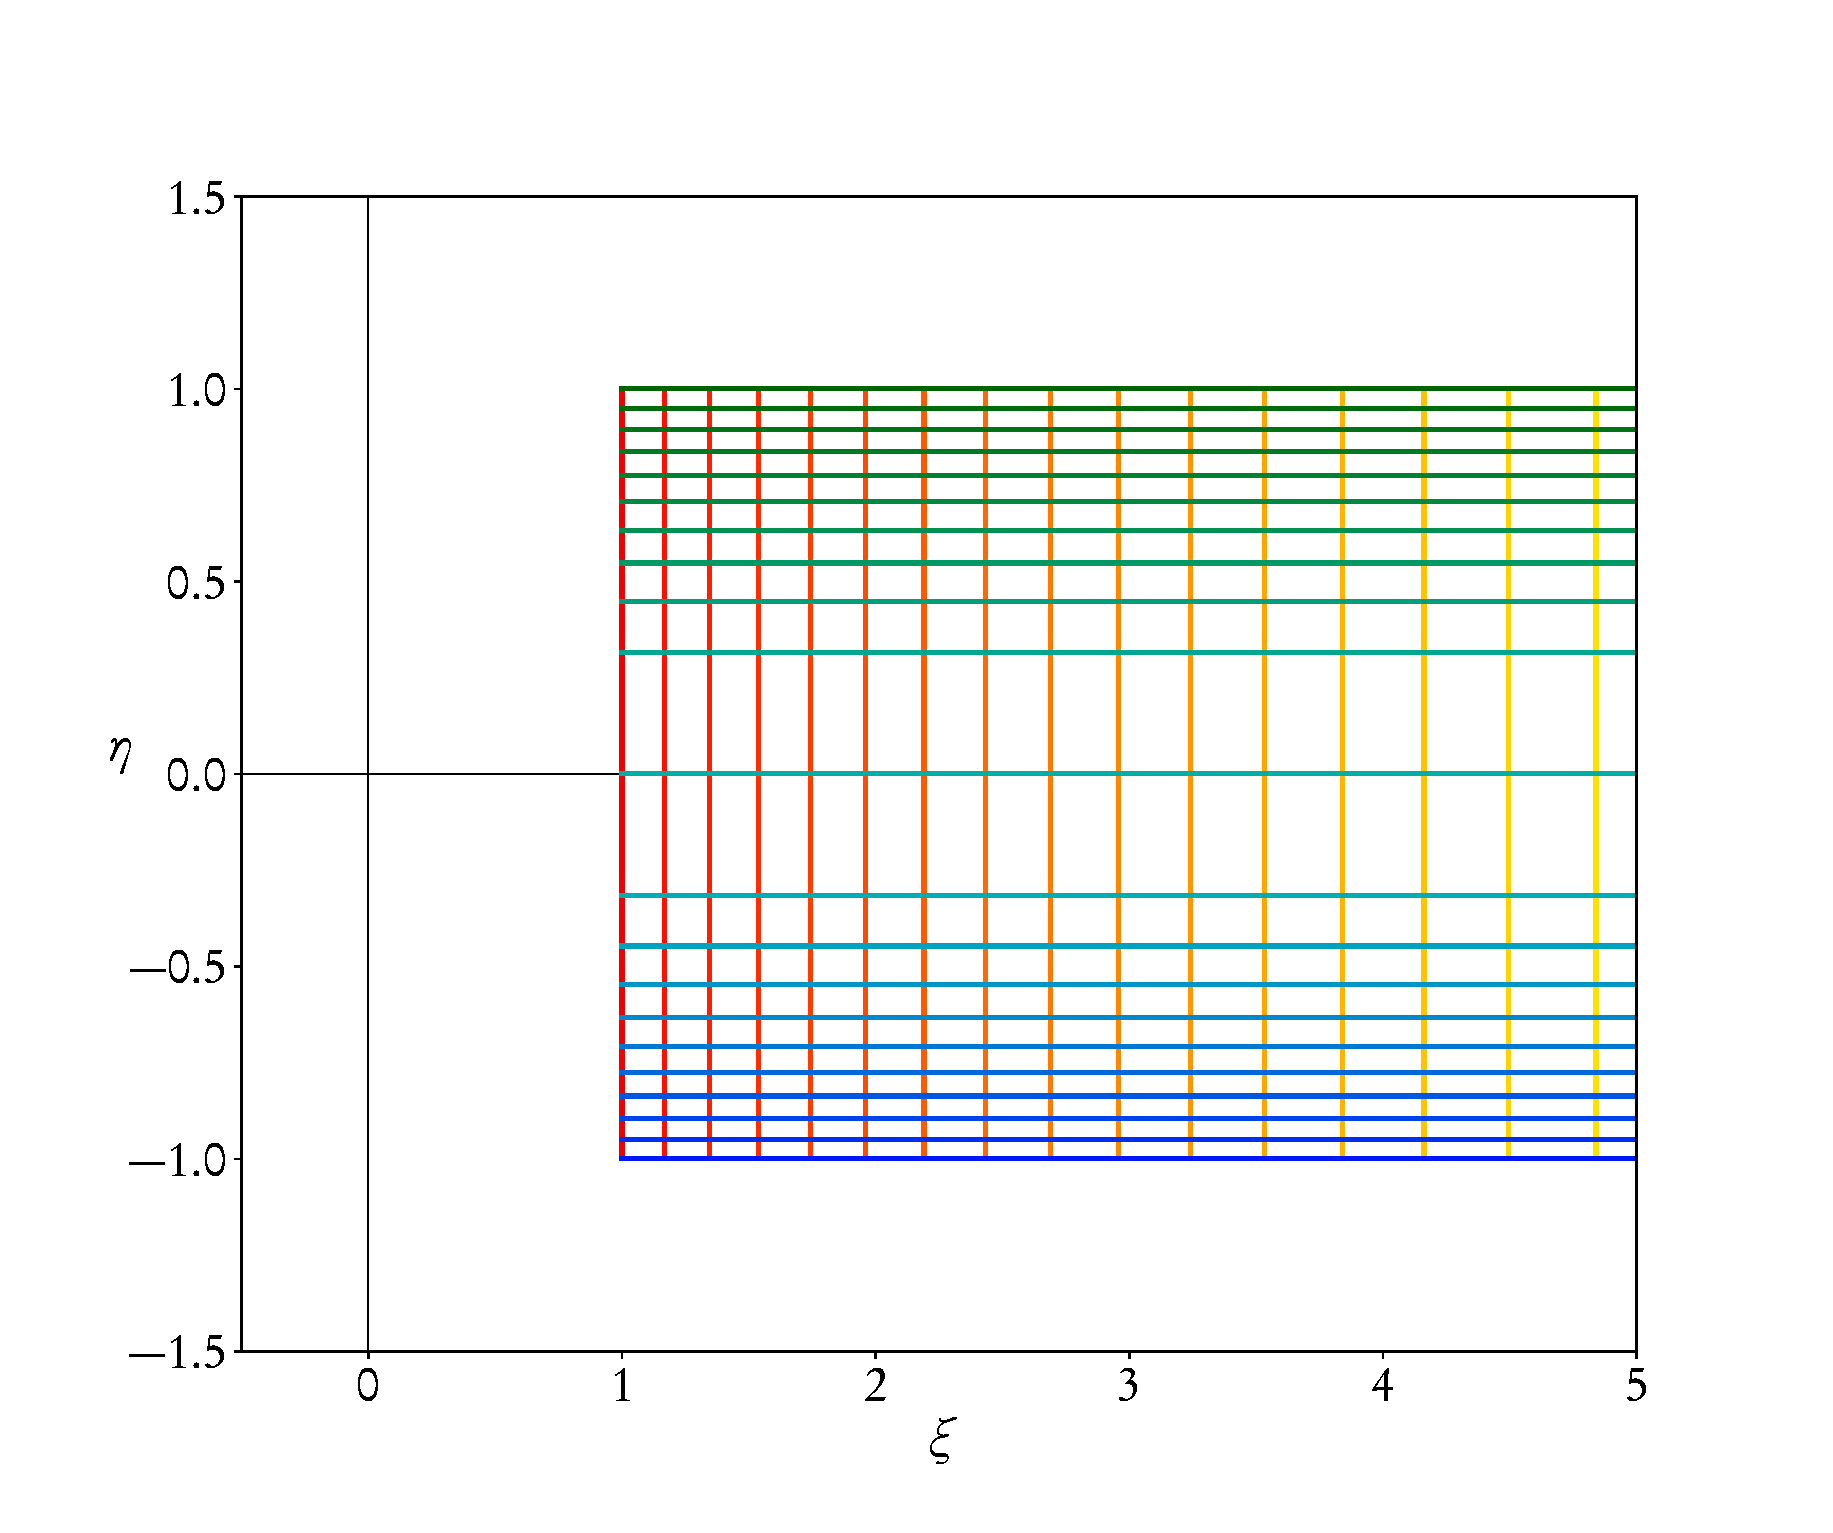
\includegraphics[width=\linewidth]{./images/appendix/xieta.eps}
               \caption{$\xi$-$\eta$ space. \label{fig:xieta}}
            \end{subfigure}%
            \begin{subfigure}{.5\textwidth}
               \centering
               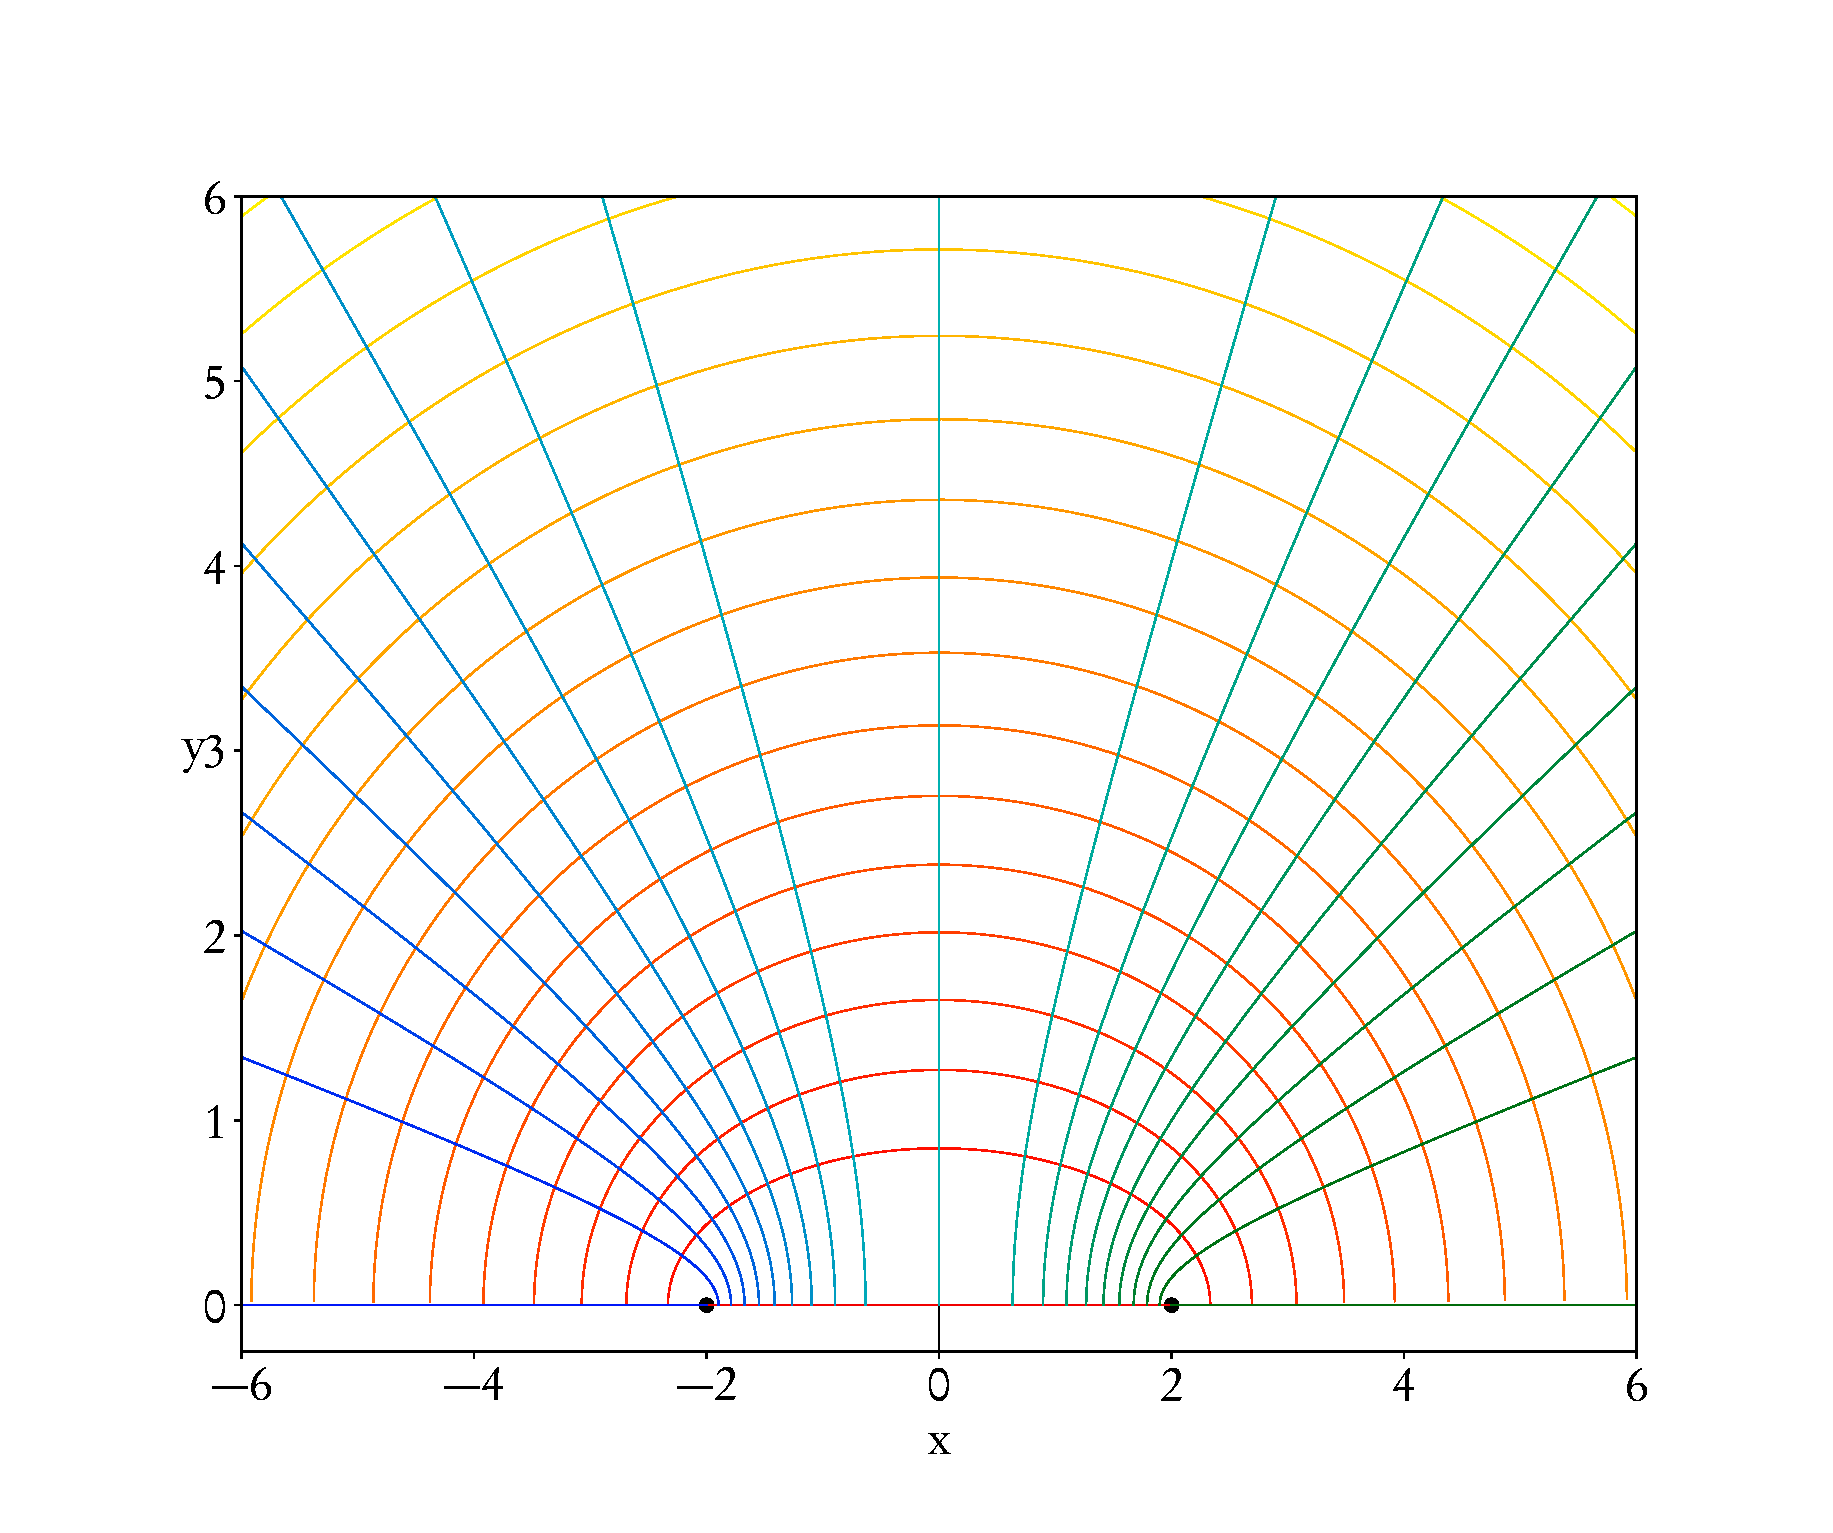
\includegraphics[width=\linewidth]{./images/appendix/eliptical.eps}
               \caption{$x$-$y$ space. \label{fig:xy}}
            \end{subfigure}
            \caption[Coordinate chart of elliptical coordinates]{The coordinate mapping of
                     Eq.~\eqref{eq:elipdef} is demonstrated by the correspondence between
                     coloured grid lines.\label{fig:elliptic}}
         \end{figure}

         Elliptical coordinates are formed by the intersection of series of confocal ellipses and
         hyperbole. If we let $(\xi, \eta)$ denote the elliptic and hyperbolic grid lines and $a > 0$
         their focal length we can cover the plane with two charts. The first is given by
         %
         \begin{equation} \label{eq:elipdef}
            \left\{
            \begin{array}{l}
               x   = a \xi \eta \\
               y^2 = a \left( \xi^2 - 1 \right) \left( 1 - \eta^2 \right),
            \end{array}
            \right.
         \end{equation}
         %
         while the second is defined similarly and covers the lower half space ($(\xi,\eta) \mapsto
         (x,-y)$). Both charts are defined for $(\xi,\eta) \in [1, \infty] \times [-1,1]$.

         This mapping is demonstrated in Fig.~\ref{fig:elliptic}. The coloured lines in the left panel
         represent a selection of $\xi$ (blues and greens) and $\eta$ (reds and oranges) grid lines.
         Grid lines are mapped by Eq.~\eqref{eq:elipdef} to lines of corresponding colour in the right
         panel.

      \end{section}

      \begin{section}{Prolate Speroidal Coordinates \label{sec:prolate}}

         Prolate spheroidal coordinates are a three-dimensional coordinate system that result from
         rotating the upper half space elliptical coordinates (defined in the proceeding section) around
         the line running through the co-foci of the elliptic and hyperbolic grid lines.

         While several conventions exist, throughout this work prolate spheroidal coordinates are
         defined as
         %
         \begin{equation} \label{eq:psc}
            \left\{
            \begin{array}{l}
               x = a \sqrt{(\xi^2 - 1)(1 - \eta^2)} \sin \phi, \\
               y = a \sqrt{(\xi^2 - 1)(1 - \eta^2)} \cos \phi, \\
               z = a \xi \eta,
            \end{array}
            \right.
         \end{equation}
         %
         for $(\xi, \eta, \phi) \in [1, \infty) \times [-1,1] \times [0,2\pi)$.

         One says that a function $f: \mathbb{R}^3 \rightarrow \mathbf{R}$ is cylindrically symmetric if
         it has no $\phi$ dependence, i.e.\ if $f(\xi,\eta,\phi) = f(\xi,\eta)$.

      \end{section}

   \end{chapter}

\end{appendices}

\cleardoublepage
\phantomsection
\addcontentsline{toc}{chapter}{References}

\singlespacing

\printbibliography[title=References] %nnnote: check references for accuracy.

\end{document}

